\documentclass{article}
\usepackage{eason}
\usepackage{pdfpages}
\usepackage[a4paper, margin=1in]{geometry}

\newcommand{\scheduleSection}[3]{\noindent\textbf{#1}\\\noindent#3 \hfill[#2]\bigbreak}
\newcommand{\contentSection}[2]{\noindent#2 \hfill[#1]\bigbreak}

\numberwithin{equation}{section}

\newcommand{\Part}{IA}
\newcommand{\Department}{DPMMS}
\newcommand{\Course}{Analysis I}
\newcommand{\Term}{Lent Term}
\newcommand{\Year}{2026}
\newcommand{\Lecturer}{R. Teixeira da Costa}
\newcommand{\Repo}{ia-dpmms-analysis-i-lt-2026}

\newcommand{\DATE}{dummyDate}
\newcommand{\COMMITSHA}{dummySHA}
\title{Part \Part\space\Course \\ \vspace{0.5em}
\Large{Lectured by \Lecturer} \\ \vspace{0.5em}
\Large{Delivered by \Department}}
\author{Notes by Eason Shao}
\date{\Term\space\Year}

\begin{document}
\maketitle

\textbf{Disclaimer.} These notes are not official and are not endorsed by the lecturers. They are nowhere near accurate representations of what was lectured, and in particular, all errors are almost surely mine.

\textbf{Use of Artificial Intelligence.} I am grateful to AI tools, including GitHub Copilot (Student Edition), Claude by Anthropic, and ChatGPT, for their assistance with typesetting, diagrams, and checking for typos and inaccuracies. I take full responsibility for verifying the mathematical content of these notes.

\vspace{3em}

The source code is available at \GitHubHref{EasonSYC}{\Repo}.

This PDF is available at \href{https://tripos.easonshao.com}{https://tripos.easonshao.com}.

\vspace{3em}

\textit{``Analysis is the study of things that are small/large, and to rigorously quantify how small/how large.''}

\vspace{2em}

\tableofcontents

\section*{Schedules}
\label{sec:schedules}

\scheduleSection{Limits and convergence}{6}{Sequences and series in \(\RR\) and \(\CC\). Sums, products and quotients. Absolute convergence; absolute convergence implies convergence. The Bolzano--Weierstrass theorem and applications (the General Principle of Convergence). Comparison and ratio tests, alternating series test.}

\scheduleSection{Continuity}{3}{Continuity of real- and complex-valued functions defined on subsets of \(\RR\) and \(\CC\). The intermediate value theorem. A continuous function on a closed bounded interval is bounded and attains its bounds.}

\scheduleSection{Differentiability}{5}{Differentiability of functions from \(\RR\) to \(\RR\). Derivative of sums and products. The chain rule. Derivative of the inverse function. Rolle's theorem; the mean value theorem. One-dimensional version of the inverse function theorem. Taylor's theorem from \(\RR\) to \(\RR\); Lagrange's form of the remainder. Complex differentiation.}

\scheduleSection{Power series}{4}{Complex power series and radius of convergence. Exponential, trigonometric and hyperbolic functions, and relations between them. *Direct proof of the differentiability of a power series within its circle of convergence*.}

\scheduleSection{Integration}{6}{Definition and basic properties of the Riemann integral. A non-integrable function. Integrability of monotonic functions. Integrability of piecewise-continuous functions. The fundamental theorem of calculus. Differentiation of indefinite integrals. Integration by parts. The integral form of the remainder in Taylor's theorem. Improper integrals.}
\section{Numerical Sequences and Series}
\subsection{Basics}

\begin{definition}[Sequence]
    \label{def:sequence}%
    A \term{sequence} \(\pqty{x_n}_{n \in \NN}\) on a set \(X\) is an enumerated list where each element is in \(X\).
\end{definition}

In this chapter, \(X \subseteq \RR\) or \(X \subseteq \CC\). An important example is \(X = \RR\), the real sequences. (We will see that the fact that we have an order on \(\RR\) is significant.)

What does it mean for \(\pqty{x_n}\) to converge to some \(x \in X\), or to diverge to infinity?

On convergence,
\begin{itemize}
    \item we need \(\abs{x_n - x}\) to be small, to be smaller than any given threshold \(\epsilon > 0\) that we choose;
    \item but for the comparison, only the `tail of the sequence', i.e. `larger \(n\)' behaviour matters: we can always ignore the first \(N\) terms of the sequence, for some \(N\) depending on \(\epsilon\).
\end{itemize}

On diverging to infinity,
\begin{itemize}
    \item we need \(\abs{x_n}\) to clear any threshold \(L > 0\) that we set for it;
    \item but similarly, only the `tail' matters; we can always ignore the first \(N\) terms, where \(N\) depends on \(L\).
\end{itemize}

\begin{definition}[Convergence of a Sequence]
    \label{def:seq-convergence}%
    A sequence \(\pqty{x_n}\) \term{converges} to some \(x\), finite, if
    \[
        \forall \epsilon > 0, \exists N = N \pqty{\epsilon} \in \NN, \forall n \geq N: \abs{x_n - x} < \epsilon.
    \]
    
    This is denoted by \(x_n \to x\).
\end{definition}

There are two definitions of divergence to infinity, one allows the behaviour to `spiral to infinity', and one does not. We use the latter, which is specified in the notes provided by the lecturer.

\begin{definition}[Divergence to Infinity for a Sequence]
    \label{def:seq-divergence-to-infinity}%
    A sequence \(\pqty{x_n}\) \term{diverges to infinity} if its modulus satisfies
    \[
        \forall L > 0, \exists N = N \pqty{L} \in \NN, \forall n \geq N: \abs{x_n} > L.
    \]
\end{definition}

\begin{remark}
    We can replace \(<\) by \(\leq\), we can replace \(\epsilon\) by \(2 \epsilon\), \(3 \epsilon\), and same for \(L\).
\end{remark}

\begin{remarks}[on divergence to infinity]
    Another definition of divergence to infinity (rarely seen) would require the argument part \(\frac{x_n}{\abs{x_n}}\) to converge. This definition may cause some confusion in some things that we took for granted before.

    \begin{enumerate}
        \item This definition of divergence to infinity effectively states that it diverges to infinity along some particular direction eventually.
        
        For example, the real sequence \(x_n = \pqty{-1}^{n - 1} n\) (i.e., \(1, -2, 3, -4, \ldots\)) does \emph{not} diverge to infinity. Similarly, the complex sequence \(x_n = \exp\pqty{in} \cdot n\) does \emph{not} diverge to infinity either.
        
        \item This gives examples of sequences with \(x_n \to 0\) with \(x_n \neq 0\) for all \(n\), but \(\frac{1}{x_n} \notto \infty\). We may only conclude that \(\abs{\frac{1}{x_n}} \to \infty\).
    \end{enumerate}
\end{remarks}

\begin{examples}[Example of Limits]
    \label{ex:seq-limits}
    \begin{itemize}
        \item Let \(x_n = \frac{1}{n}\), then \(x_n \to 0\), because for any given \(\epsilon > 0\), if we choose \(N = 1 + \ceil{\frac{1}{\epsilon}}\), then for all \(n \geq N\),
        \[
            \abs{x_n - 0} = \frac{1}{n} < \epsilon.
        \]

        \item Let \(x_n = \frac{1}{2^n}\), then \(x_n \to 0\), because similarly, for any given \(\epsilon > 0\), if we choose \(N = \max\Bqty{1 + \log_2 \pqty{\frac{1}{\epsilon}}, 1}\), then for all \(n \geq N\),
        \[
            \abs{x_n - 0} = \frac{1}{2^n} < \epsilon.
        \]

        \item Let \(x_n = in\), then \(x_n \to \infty\), since for any given \(L > 0\), let \(N = 1 + \ceil{L}\), then for all \(n \geq N\),
        \[
            \abs{x_n} = \abs{in} = n > L.
        \]

        \item Let \(x_n = \pqty{-1}^n\), then \(x_n\) doesn't diverge to \(\infty\) (\(\abs{x_n} \leq 1\)) but also does not converge.
    \end{itemize}
\end{examples}

\begin{lemma}[Limits of Sequences are Unique]
    \label{lem:seq-limit-unique}%
    For a sequence \(\pqty{x_n}\), if \(x_n \to a\) and \(x_n \to b\), then \(a = b\).
\end{lemma}

\begin{proof}
    Let \(x_n \to a\) and \(x_n \to b\). Let \(\epsilon > 0\) be arbitrary. We have some \(N_1 \pqty{\epsilon}\) and \(N_2 \pqty{\epsilon}\), such that
    \[
        \forall n \geq N_1\pqty{\epsilon}: \abs{x_n - a} < \epsilon
    \]
    and
    \[
        \forall n \geq N_2\pqty{\epsilon}: \abs{x_n - b} < \epsilon.
    \]

    In particular, we look at \(N\pqty{\epsilon} = \max\Bqty{N_1, N_2}\). It must still be the case that for all \(n \geq N\),
    \[
        \abs{x_n - a}, \abs{x_n - b} < \epsilon.
    \]

    Hence, for all \(n \geq N\pqty{\epsilon}\), by the triangular inequality,
    \begin{align*}
        \abs{a - b} &= \abs{a - x_n + x_n - b} \\
        &\leq \abs{x_n - a} + \abs{x_n - b} && \text{Triangular Inequality} \\
        &< 2\epsilon.
    \end{align*}

    Hence, we may conclude that \(\abs{a - b} = 0\), which shows \(a = b\).
\end{proof}

\begin{proposition}[Sandwich Theorem for Sequences]
    \label{prop:seq-sandwich-theorem}%
    Let \(\pqty{x_n}, \pqty{y_n}\) and \(\pqty{z_n}\) be real sequences. Then,
    \begin{itemize}
        \item \term{Limits preserve weak order.} If \(x_n \leq y\) for all \(n \in \NN\), and \(x_n \to x\), then \(x \leq y\);
        \item \term{Sandwich theorem.} If \(x_n \to x\) and \(z_n \to x\), and \(x_n \leq y_n \leq z_n\) for all \(n \in \NN\), then \(y_n \to x\).
    \end{itemize}
\end{proposition}

\begin{remark}
    In the first part for \emph{limits preserve weak order}, note that \emph{limits does not preserve strong order}, i.e. we \emph{cannot} replace all \(\leq\)s with \(<\)s. Even if \(x_n < y\) for all \(n \in \NN\), we can only conclude \(x_n \to x \leq y\) if it converges.
\end{remark}

\begin{proof}[\proofname\ of \autoref{prop:seq-sandwich-theorem}]
    \begin{itemize}
        \item Suppose for contradiction that \(y < x\), and let \(\epsilon = x - y > 0\). Now, there must be some \(N \in \NN\), such that for all \(n \geq N\),
        \[
            \abs{x_n - x} < \epsilon,
        \]
        and in particular, \(x_n > x - \epsilon = y\). This contradicts with the assumption.

        \item By definition, for all \(\epsilon > 0\), there is some \(N \in \NN\) such that for all \(n \geq N\),
        \[
            \abs{x_n - x}, \abs{z_n - x} < \epsilon.
        \]

        In particular, since \(x_n \leq y_n \leq z_n\), we have
        \[
            \abs{y_n - x} < \epsilon
        \]
        and this finishes the proof.
    \end{itemize}
\end{proof}

Having proved this, this allows us to show that the sequences have a unique limit in another way.

\begin{proof}[\proofname\ to \autoref{lem:seq-limit-unique}, using \autoref{prop:seq-sandwich-theorem} (Sandwich Theorem)]
    Using the triangular inequality, we have
    \[
        0 \leq \abs{a - b} \leq \abs{a - x_n} + \abs{b - x_n}.
    \]

    Taking the limit as \(n \to \infty\) and applying \autoref{prop:seq-sandwich-theorem} (Sandwich Theorem) shows that \(0 \leq \abs{a - b} \leq 0\), showing \(a = b\) as desired.
\end{proof}

\begin{lemma}[Convergence in \(\CC\) is the same as Convergence in \(\RR\) for Sequences]
    \label{lem:seq-convergence-in-c}%
    Let \(\pqty{x_n}\) be a complex sequence. Then \(x_n \to x\) if and only if \(\Re\pqty{x_n} \to \Re\pqty{x}\), and \(\Im \pqty{x_n} \to \Im\pqty{x}\).
\end{lemma}

\begin{proof}
    Recall that for some \(z \in \CC\), we have that
    \[
        \abs{z} = \sqrt{\pqty{\Re z}^2 + \pqty{\Im z}^2}.
    \]
    
    \(\implies\). We use inequalities
    \[
        \abs{\Re z}, \abs{\Im z} \leq \abs{z}.
    \]

    Now, since \(x_n \to x\), for all \(\epsilon > 0\), there is some \(N = N\pqty{\epsilon} \in \NN\), such that for all \(n \geq N\),
    \[
        \abs{x_n - x} < \epsilon.
    \]

    Now, note that
    \[
        \abs{\Re\pqty{x_n} - \Re\pqty{x}}, \abs{\Im\pqty{x_n} - \Im\pqty{x}} \leq \abs{x_n - x} < \epsilon,
    \]
    and so \(\Re\pqty{x_n} \to \Re\pqty{X}\), and \(\Im\pqty{x_n} \to \Im\pqty{x}\).

    \(\impliedby\). Note the inequality
    \[
        \abs{z} \leq \abs{\Re z} + \abs{\Im z}.
    \]

    Let \(\epsilon > 0\) be arbitrary. Then, there is some \(N_1 = N_1 \pqty{\epsilon}\) and \(N_2 = N_2 \pqty{\epsilon}\), such that
    \[
        \forall n \geq N_1, \abs{\Re\pqty{x_n} - \Re\pqty{x}} < \epsilon
    \]
    and
    \[
        \forall n \geq N_2, \abs{\Im\pqty{x_n} - \Im\pqty{x}} < \epsilon.
    \]

    Hence, for all \(n \geq \max\Bqty{N_1, N_2}\),
    \begin{align*}
        \abs{x_n - x} &= \abs{\pqty{\Re \pqty{x_n} - \Re \pqty{x}} + i \pqty{\Im \pqty{x_n} - \Im \pqty{x}}} \\
        &\leq \abs{\Re\pqty{x_n} - \Re\pqty{x}} + \abs{i\pqty{\Im\pqty{x_n} - \Im\pqty{x}}} && \text{triangular inequality} \\
        &= \abs{\Re\pqty{x_n} - \Re\pqty{x}} + \abs{\Im\pqty{x_n} - \Im\pqty{x}} \\
        &< 2\epsilon
    \end{align*}
    showing as desired.
\end{proof}

\begin{definition}[Bounded Sequence]
    \label{def:seq-bounded}%
    We say \(\pqty{x_n}\) is \term{bounded}, if there is some \(M > 0\), such that for all \(n \in \NN\), that
    \[
        \abs{x_n} \leq M.
    \]

    Equivalently, if there is some \(M > 0\), such that
    \[
        \sup_{n \geq 0} \abs{x_n} \leq M.
    \]
\end{definition}

\begin{lemma}[Convergent Sequences are Bounded]
    \label{lem:seq-convergence-bounded}%
    If \(x_n \to x\), then \(\pqty{x_n}\) must be bounded.
\end{lemma}

\begin{proof}
    Take \(\epsilon = 1\), and hence there is some \(N \in \NN\), such that
    \[
        \forall n \geq N: \abs{x_n - x} \leq 1.
    \]

    Hence, it must be the case that
    \[
        \forall n \geq N: \abs{x_n} \leq 1 + \abs{x}
    \]
    which gives a bound on \(x_n\) for sufficiently large \(n\). For the remaining finite number of elements, we have for all \(1 \leq n \leq N\),
    \[
        \abs{x_n} \leq \max_{1 \leq n \leq N} \abs{x_n} < \infty.
    \]

    This gives an overall bound of
    \[
        \abs{x_n} \leq \max\Bqty{\max_{1 \leq n \leq N} \abs{x_n}, \abs{x} + 1}.
    \]
\end{proof}

\begin{lemma}[Limits preserve Arithmetic for Sequences]
    \label{lem:seq-limits-arithmetic}%
    Let \(x_n \to x\) and \(y_n \to y\). Then \(x_n + y_n \to x + y\) and \(x_n y_n \to xy\). Furthermore, if \(x \neq 0\), then \(\frac{1}{x_n} \to \frac{1}{x}\).
\end{lemma}

\begin{proof}[\proofname\ for the Sum]
    We note that if \(x_n \to x\) and \(y_n \to y\), let the \(N \in \NN\) for \(\epsilon > 0\) be \(N_1\pqty{\frac{\epsilon}{2}}\) and \(N_2\pqty{\frac{\epsilon}{2}}\). Therefore, for all \(n \geq \max\Bqty{N_1, N_2}\),
    \[
        \abs{\pqty{x_n + y_n} - \pqty{x + y}}
        \leq \abs{x_n - x} + \abs{y_n - y} < \frac{\epsilon}{2} + \frac{\epsilon}{2} = \epsilon.
    \]
    and this finishes the proof for the sum.
\end{proof}

\begin{proof}[\proofname\ for the Product]
    Notice that
    \begin{align*}
        \abs{x_n y_n - xy} &= \abs{x_n y_n - x y_n + x y_n - xy} \\
        &\leq \abs{x} \abs{y_n - y} + \abs{y_n} \abs{x - x_n}. && \text{Triangular Inequality}
    \end{align*}

    For any \(\epsilon > 0\), there exists \(N_1 = N_1 \pqty{\epsilon}\) and \(N_2 = N_2 \pqty{\epsilon}\), such that
    \begin{itemize}
        \item \(\abs{x_n - x} < \epsilon\) for all \(n \geq N_1\); and
        \item \(\abs{y_n - y} < \epsilon\) for all \(n \geq N_2\).
    \end{itemize}

    Hence, for any \(n \geq \max\Bqty{N_1, N_2}\), we have
    \[
        \abs{x_n y_n - xy} < \epsilon \pqty{\abs{x} + \abs{y_n}}.
    \]

    Hence, by \autoref{lem:seq-convergence-bounded}, we may replace \(\abs{y_n}\) with some bound on it, and so we are done.
\end{proof}

\begin{proof}[\proofname\ for the Reciprocal]
    Take \(\epsilon = \frac{1}{2} \abs{x}\), then let \(N \in \NN\) such that for all \(n \geq N\), we have
    \[
        \abs{x_n - x} < \epsilon = \frac{1}{2} \abs{x},
    \]
    then we certainly have \(\abs{x_n} > \frac{1}{2} \abs{x}\).

    Let \(\delta > 0\) be arbitrary. Take \(M \in \NN\) such that for all \(n \geq M\), we have
    \[
        \abs{x_n - x} < \frac{1}{2} \abs{x}^2 \delta.
    \]

    Hence, for \(n \geq \max\Bqty{N, M}\)
    \begin{align*}
        \abs{\frac{1}{x_n} - \frac{1}{x}} = \abs{\frac{x - x_n}{x x_n}} < \frac{2}{\abs{x}^2} \abs{x - x_n} < \delta
    \end{align*}
    which finishes our proof.
\end{proof}

Note that most of the \(n \in \NN\) above can be replaced with \(n\) sufficiently large -- since every time when we consider limits, we in fact only consider the behaviour for sufficiently large \(n\).

\begin{definition}[Monotone Sequence]
    \label{def:seq-monotone}%
    We say a real sequence \(\pqty{x_n}\) is \term{monotone}, if either
    \begin{itemize}
        \item it is \term{increasing}: \(x_n \leq x_{n + 1}\) for all \(n \in \NN\); or
        \item it is \term{decreasing}: \(x_n \geq x_{n + 1}\) for all \(n \in \NN\).
    \end{itemize}

    \term{Strictly monotone} is when we replace the \(\leq, \geq\) symbols with \(<, >\).
\end{definition}

Similarly, if we attempt to conclude some limiting behaviour of a sequence that is \emph{eventually} monotone, then we can apply any theorem on a monotone sequence, since we only care about large \(n\) behaviours. An example of such a theorem is \autoref{thm:monotone-convergence}.

\begin{theorem}[Monotone Convergence Theorem]
    \label{thm:monotone-convergence}%
    Bounded monotone real sequence converges.
\end{theorem}

\begin{proof}
    Without loss of generality, assume that the sequence is strictly increasing. Use the supremum axiom of \(\RR\) that every non-empty subset of \(\RR\) that is bounded above has a supremum in \(\RR\), and we would like to show that such supremum of the elements of the sequence is in fact the limit. (Numbers and Sets provide details for the proof.)
\end{proof}

\subsection{Bolzano--Weierstrass Theorem}

We cannot say this about sequences that are bounded but not (eventually) monotonic. Indeed, from previously, the sequence \(\pqty{x_n} = \pqty{-1}^n\) is bounded with \(\abs{x_n} \leq 1\), but it does not converge. However,
\begin{itemize}
    \item if we delete the even terms: \(x_{2k + 1} = -1\) converge to \(-1\); and
    \item if we delete the odd terms: \(x_{2k} = 1\) converge to \(1\).
\end{itemize}

The constant subsequences converge. But is it necessary that some subsequence converges for \emph{every} sequence? We first formally define what a subsequence is.

\begin{definition}[Subsequence]
    \label{def:seq-subsequence}%
    Given a sequence \(\pqty{x_n}\), a \term{subsequence} of \(x_n\) is a sequence \(\pqty{x_{n_k}}_{k \in \NN}\), where \(\pqty{n_k}_{k \in \NN}\) is a strictly increasing natural number sequence.
\end{definition}

Now we are ready to give the main result of this section.

\begin{theorem}[Bolzano--Weierstrass Theorem]
    \label{thm:bolzano-weierstrass}%
    If \(\pqty{x_n}\) is a real, bounded sequence, then it has at least one convergent subsequence.
\end{theorem}

The example above with \(\pqty{-1}^n\) shows that there could be more subsequences, and the limits could be different.

To prove this result, we first give the following lemmas which are useful.

\begin{lemma}[Subsequences Converge to the Same Limit]
    \label{lem:seq-subsequence-same-limit}%
    If \(x_n \to x\), then any subsequence \(\pqty{x_{n_k}}\) of \(\pqty{x_n}\) must converge to the same limit.
\end{lemma}

\begin{proof}
    Since \(n_k < n_{k + 1}\), this shows that \(n_{k + 1} \geq n_k + 1\). By induction, we can show that \(n_k \geq k\).

    Take \(\epsilon > 0\) to be positive. Since \(x_n \to x\), let \(N = N\pqty{\epsilon}\) be such that
    \[
        \forall n \geq N: \abs{x_n - x} < \epsilon.
    \]

    So, if we let \(k \geq N\), then \(n_k \geq k \geq N\), so
    \[
        \abs{x_{n_k} - x} < \epsilon,
    \]
    showing that \(x_{n_k} \to x\) as \(k \to \infty\).
\end{proof}

\begin{theorem}[Nested Interval Theorem]
    \label{thm:nested-interval-thm}%
    Let \(\pqty{I_n}_{n \in \NN}\) be a sequence of nested closed intervals in \(\RR\), i.e. \(I_n \supseteq I_{n + 1}\) for all \(n \in \NN\). Let \(I_n = \ccintv{a_n}{b_n}\). If \(b_n - a_n = \abs{I_n} \to 0\) as \(n \to \infty\), then the intersection
    \[
        \bigcap_{n \in \NN} I_n
    \]
    contains exactly one point in \(\RR\).
\end{theorem}

\begin{proof}
    Since the intervals \(I_n \supseteq I_{n + 1}\), we have
    \begin{itemize}
        \item \(a_n \leq a_{n + 1}\); and
        \item \(b_n \geq b_{n + 1}\)
    \end{itemize}
    for all \(n \in \NN\). Furthermore, since \(I_1 \supseteq I_n\), we have
    \[
        a_1 \leq a_n \leq b_n \leq b_1.
    \]

    This gives that \(\pqty{a_n}\) is increasing, and bounded above by \(b_1\); and that \(\pqty{b_n}\) is decreasing, and bounded below by \(a_1\).

    Hence, by \autoref{thm:monotone-convergence} (Monotone Convergence Theorem), there exists \(a, b \in \RR\), such that \(a_n \to a\) and \(b_n \to b\).
    
    By \autoref{prop:seq-sandwich-theorem} (Sandwich Theorem), since limits preserve inequalities, we have \(a \leq b\) in the limit.

    We show next the existence of an element in the intersection -- i.e. the intersection is not trivial. We fix an arbitrary \(n \in \NN\). For all \(k \geq n\), we have \(a_k \in \ccintv{a_k}{b_k} \subseteq \ccintv{a_n}{b_n}\), which shows that \(a_n \leq a_k \leq b_n\). Hence, by applying \autoref{prop:seq-sandwich-theorem} (Sandwich Theorem), let \(k \to \infty\), and we have \(a_n \leq a \leq b_n\). This holds true for any \(n \in \NN\), so \(a \in I_n\) for any \(n \in \NN\), which shows that
    \[
        a \in \bigcap_{n \in \NN} I_n.
    \]

    To show that this is the only element in the infinite intersection, note that \(b_n - a_n \to b - a\) from \autoref{lem:seq-limits-arithmetic} (Limits Preserve Arithmetic), and we have \(b_n - a_n \to 0\). Since \autoref{lem:seq-limit-unique} (limits are unique), we deduce that \(b - a = 0\), so \(a = b\).

    Hence, for any \(x \in \bigcap_{n \in \NN} I_n\), we have \(a_n \leq x \leq b_n\), and taking the limit as \(n \to \infty\), by using \autoref{prop:seq-sandwich-theorem}, we see that \(a \leq x \leq b\), and hence \(x = a = b\).

    This finishes our proof.
\end{proof}

Now, we prove \autoref{thm:bolzano-weierstrass} (Bolzano--Weierstrass). We find an algorithm that works for \emph{any} sequence that extracts a convergent subsequence.

\begin{proof}[\proofname\ of \autoref{thm:bolzano-weierstrass} (Bolzano--Weierstrass), using Nested Interval Theorem]
    We are given \(\pqty{x_n}\) and its bound, say \(M > 0\), such that \(\abs{x_n} \leq M\) for all \(n \in \NN\). We want to construct a sequence of nested intervals, from which we can sample our subsequence, since that would ensure our subsequence would converge, to the unique intersection point of the nested intervals.

    Let \(a_1 = -M, b_1 = +M\), so \(I_1 = \ccintv{-M}{M} \supseteq \set{x_n}{n \in \NN}\).

    Now, take \(c = \frac{a_1 + b_1}{2}\). Then, at least one of the halves \(\ccintv{a_1}{c}\) and \(\ccintv{c}{b_2}\) will have infinitely many elements of the sequence. Take \(I_2\) to be a half to have infinitely many elements.

    We continue this inductively, and we will get a sequence \(\pqty{I_n}_{n \in \NN}\). By construction, this is clearly a sequence of nested intervals, and they have infinitely many elements of the sequence each. The length of the interval halves each time, so the limit of the width of the intervals is zero.

    Therefore, by \autoref{thm:nested-interval-thm} (Nested Interval Theorem), we see that there is a unique \(x \in \RR\) such that \(\bigcap_{n \in \NN} I_n = \Bqty{x}\).

    We choose \(\pqty{x_{n_k}}\) as follows. Pick \(n_1 \in \NN\) such that \(x_{n_1} \in I_1\). Then, \(I_2\) has an infinite intersection with \(\set{x_n}{n > n_1}\).

    Now, we pick \(n_2 > n_1\) such that \(x_{n_2} \in I_2\). We may continue this inductively to get \(\pqty{x_{n_k}}_{k \in \NN}\).

    We have \(a_k \leq x_{n_k} \leq b_k\), so taking the limit as \(k \to \infty\), by \autoref{prop:seq-sandwich-theorem} (Sandwich Theorem), gives that \(x \leq \lim_{k \to \infty} x_{n_k} \leq x\), and hence \(\lim_{k \to \infty} x_{n_k} = x\), as desired.
\end{proof}

\begin{remark}
    One may be tempted to conclude the proof by for all \(k \in \NN\), we have \(x_{n_k} \in I_k\), and hence
    \[
        x_{n_k} \in \bigcap_{n \leq k} I_n,
    \]
    and the result then follows (maybe by taking a limit \(k \to \infty\)). However, this does depend on certain topological properties on the sets \(I_n\), and note that an infinite intersection is not about taking some limit, so the proof using \autoref{prop:seq-sandwich-theorem} (Sandwich Theorem) is included.
\end{remark}

\begin{proof}[\proofname\ of \autoref{thm:bolzano-weierstrass} (Bolzano--Weierstrass), using \autoref{thm:monotone-convergence} (Monotone Convergence Theorem)]
    We first consider the set of indices
    \[
        P = \set{n \in \NN}{\forall m \geq n: x_m \geq x_n}.
    \]

    If such set is infinite, say \(P = \Bqty{n_1, n_2, \ldots} \subseteq \NN\) for \(n_1 < n_2 < n_3 < \cdots\), then the subsequence \(\pqty{x_{n_t}}_{t \in \NN}\) is an increasing sequence.

    Now we assume such set is finite, and let \(N = \max P\). For all \(n > N\), we have \(n \notin P\), and hence
    \[
        \exists m = m\pqty{n} \geq n: x_m < x_n.
    \]

    We construct a subsequence recursively as follows. Let \(n_1 = n + 1\), and let \(n_2 = m\pqty{n_1} \geq n_1 > B\), \(n_3 = m\pqty{n_2} \geq n_2 > N\), etc. This creates a (strictly) decreasing subsequence \(\pqty{x_{n_t}}_{t \in \NN}\).

    Applying \autoref{thm:monotone-convergence} (Monotone Convergence Theorem) and using the bounded assumption gives us a convergent subsequence as desired.
\end{proof}

The Bolzano--Weierstrass theorem for Complex Sequences hold as well. We can use
\[
    x_n = \Re x_n + i \Im x_n
\]
and apply the real version of the Bolzano--Weierstrass to the real and complex parts, one after another. (Alternatively, a similar mechanism may also be applied to the real and complex parts simultaneously.)

An interesting application of Bolzano--Weierstrass Theorem is the following proposition.

\begin{proposition}[Convergence via Subsequences]
    \label{prop:convergence-via-subsequences}%
    Let \(\pqty{x_n}\) be bounded. If all convergent subsequences converge to the same limit, then \(x_n\) converges to the same limit.

    In other words, if \(x_n\) does not converge, then there are two convergent subsequences that converge to different limits.
\end{proposition}

\begin{proof}
    We proof the contrapositive. By Bolzano--Weierstrass theorem, since the sequence \(\pqty{x_n}\) is bounded, there is some subsequence of \(\pqty{x_n}_{n \in \NN}\), say \(\pqty{x_{n_k}}_{k \in \NN}\), that converges to some limit \(L\).

    We aim to construct another subsequence that does not converge to \(L\). Since \(\pqty{x_n}\) diverges, in particular, \(x_n \notto L\), and hence for some \(\epsilon > 0\), we have
    \[
        \forall N \in \NN, \exists n = n\pqty{N} > N: \abs{x_n - L} > \epsilon.
    \]

    We recursively define a new subsequence \(\pqty{x_{m_k}}_{k \in \NN}\) as follows.

    For \(k = 1\), let \(N_1 = 1\), and let \(m_1 = n\pqty{N_1} > N_1\).
    
    For \(k = 2\), let \(N_2 = m_1\), and let \(m_2 = n\pqty{N_2} > N_2\). And this continues on.

    Note that \(\pqty{m_k}_{k \in \NN}\) is indeed strictly increasing, and \(\pqty{x_{m_k}}_{k \in \NN}\) must be bounded. Applying Bolzano--Weierstrass on this subsequence gives some convergent \(\pqty{x_{m_{k_t}}}_{t \in \NN}\), say \(x_{m_{k_t}} \to L'\) as \(t \to \infty\).
    
    But since for the previous \(\epsilon\), we have \(\abs{x_{m_k} - L} > \epsilon\) for all \(k \in \NN\), and in particular, \(\abs{x_{m_{k_t}} - L} > \epsilon\) for all \(t \in \NN\), so it is impossible for \(L' = L\).
\end{proof}

\subsection{Cauchy Sequences}

\begin{definition}[Cauchy Sequence]
    \label{def:seq-cauchy}%
    A sequence \(\pqty{x_n}\) is \term{Cauchy} if
    \[
        \forall \epsilon > 0, \exists N = N \pqty{\epsilon} \in \NN, \forall m, n \geq N: \abs{x_m - x_n} < \epsilon.
    \]

    Intuitively, a sequence is Cauchy if any two terms can be arbitrarily close in the tail.
\end{definition}

\begin{examples}[Cauchy and Non-Cauchy Sequences]
    \label{ex:seq-cauchy}
    \begin{itemize}
        \item Consider \(x_n = \frac{1}{n}\). Without loss of generality, assume \(m \geq n\). Let \(\epsilon > 0\) be arbitrary, we want to have
        \[
            \abs{x_m - x_n} = \abs{\frac{1}{m} - \frac{1}{n}} = \frac{1}{n} - \frac{1}{m} = \frac{m - n}{mn} \leq \frac{1}{n} < \epsilon.
        \]

        Therefore, let \(N\pqty{\epsilon} = \ceil{\frac{1}{\epsilon}} + 1\), then this desired inequality holds. So this sequence is Cauchy.

        \item Consider \(x_n = \pqty{-1}^{n}\) is \emph{not} Cauchy. Indeed, take \(n = 2k\) and \(m = 2k + 1\) for any \(k \in \NN\), then
        \[
            \abs{x_n - x_m} = 2.
        \]

        Therefore, for example, for \(\epsilon = 1\), the definition must fail.

        \item Consider a sequence \(\pqty{x_n}\) on \(\QQ\) which is given by the truncation of the decimal expansion of \(\sqrt{2}\): so
        \[
            x_1 = 1, x_2 = 1.4, x_3 = 1.41, x_4 = 1.414, \ldots
        \]

        We claim this is Cauchy. Without loss of generality, let \(m > n\), then
        \[
            \abs{x_m - x_n} < 10^{-\pqty{n - 1}} < \epsilon
        \]
        for sufficiently large \(m, n\). Alternatively, note
        \[
            10^{-\pqty{n - 1}} \to 0
        \]
        which shows it is Cauchy as well.

        This sequence does \emph{not} converge over \(\QQ\). However, it does converge over \(\RR\), to \(\sqrt{2}\).
    \end{itemize}
\end{examples}

However, if \(\pqty{x_n}\) only satisfies that
\[
\forall \epsilon > 0, \exists N = N\pqty{\epsilon} \in \NN, \forall n \geq N: \abs{x_n - x_{n + 1}} < \epsilon,
\]
must it be the case that \(\pqty{x_n}\) is Cauchy? Note that this definition is equivalent to 
\[
    x_n - x_{n + 1} \to 0,
\]
so it is not hard to see that there will be some counterexample to this.

\begin{lemma}[Cauchy Sequences are Bounded]
    \label{lem:seq-cauchy-sequences-are-bounded}%
    If \(\pqty{x_n}\) is Cauchy, then it is bounded.
\end{lemma}

\begin{proof}
    We can simply take the definition for \(\epsilon = 1\). Then there is some \(N \in \NN\), such that for all \(n, m \geq N\), we have
    \[
        \abs{x_n - x_m} < \epsilon = 1.
    \]

    We fix \(m = N\). For all \(n \geq N\), we have
    \[
        \abs{x_n - x_N} < 1.
    \]

    This shows that
    \[
        \abs{x_n} < 1 + \abs{x_N},
    \]
    and since \(x_N\) is a fixed real number, this shows that it is bounded on the tail.
\end{proof}

\begin{lemma}[Complex Cauchy Sequences]
    \label{lem:seq-cauchy-complex-real}%
    A complex sequence \(\pqty{x_n}\) is Cauchy, if and only if the real sequences \(\Re x_n\) and \(\Im x_n\) are Cauchy.
\end{lemma}

\begin{lemma}[Convergent Sequences are Cauchy]
    \label{lem:seq-convergent-implies-cauchy}%
    If \(x_n \to x\), then \(x_n\) is Cauchy.
\end{lemma}

\begin{proof}
    By the triangular inequality, we have
    \[
        \abs{x_n - x_m} = \abs{x_n - x + x - x_m} \leq \abs{x_n - x} + \abs{x_m - x}.
    \]

    Since \(x_n \to x\), for all \(\epsilon > 0\), we have \(N = N\pqty{\epsilon} \in \NN\), such that for all \(n \geq N\),
    \[
        \abs{x_n - x} < \epsilon.
    \]

    Let \(\epsilon > 0\) be arbitrary, and let \(m, n \geq N\pqty{\epsilon}\). We have
    \[
        \abs{x_n - x_m} \leq \abs{x_n - x} + \abs{x_m - x} \leq 2 \epsilon
    \]
    which finishes the proof.
\end{proof}

Is the converse necessarily true? Note the above example on \(\sqrt{2}\) gives an example of a Cauchy sequence on \(\QQ\) that do \emph{not} converge on \(\QQ\). This can only be true for `nice' subsets of \(\CC\).

\begin{theorem}[Completeness of \(\RR\) and \(\CC\) / Cauchy Sequences are Convergent on \(\RR\) or \(\CC\)]
    \label{thm:completeness-of-r-and-c}%
    Every Cauchy sequence on \(\RR\) or \(\CC\) is convergent.
\end{theorem}

\begin{remark}
    This allows for a proof of convergence of sequences in \(\RR\) or \(\CC\), without having to guess what the limit is.
\end{remark}

\begin{proof}[\proofname\ of \autoref{thm:completeness-of-r-and-c} (Cauchy Sequences are Convergent on \(\RR\) or \(\CC\))]
    It is sufficient to show that this is true for real sequences, by \autoref{lem:seq-convergence-in-c} and \autoref{lem:seq-cauchy-complex-real}. (The proof itself, however, does not rely on the sequence being real.)

    We have seen that \(\pqty{x_n}\) is Cauchy implies \(\pqty{x_n}\) is bounded, from \autoref{lem:seq-cauchy-sequences-are-bounded}.
    
    By \autoref{thm:bolzano-weierstrass} (Bolzano--Weierstrass Theorem), there is some subsequence \(\pqty{x_{n_k}}\) that converges to some \(x\).

    By the triangular inequality, we have
    \[
        \abs{x_n - x} \leq \abs{x_n - x_{n_k}} + \abs{x_{n_k} - x}.
    \]

    The first absolute value could then be dealt with the fact that the sequence is Cauchy, and the second by that the subsequence converges.

    More precisely, let \(\epsilon > 0\) be arbitrary. Since \(\pqty{x_n}\) is Cauchy, we have some \(N_1 = N_1 \pqty{\epsilon}\), such that for all \(m, n \geq N_1\),
    \[
        \abs{x_n - x_m} < \epsilon.
    \]

    In particular, take \(m = n_k \geq N_1\), we have
    \[
        \abs{x_n - x_{n_k}} < \epsilon
    \]
    for all \(n, n_k \geq N_1\).

    On the other hand, since \(x_{n_k} \to x\), there is some \(N_2 = N_2 \pqty{\epsilon}\), such that for all \(k \geq N_2\), we have
    \[
        \abs{x_{n_k} - x} < \epsilon.
    \]

    We fix \(k \geq N_2\) such that \(n_k \geq N_1\), then
    \[
        \abs{x - x_n} < 2\epsilon
    \]
    for all \(n \geq N_1\). This gives \(x_n \to x\).
\end{proof}

\begin{remark}
    Metric spaces in which Cauchy sequence implies convergence is called \term{complete}. \(\QQ\) is \emph{not} a complete metric space. In fact, \(\RR\) is the \emph{only} complete, ordered field (up to isomorphism).
\end{remark}

\subsection{Series and Convergence Tests}

\begin{definition}[Series]
    Let \(\pqty{a_n}_{n \in \NN}\) be a sequence over \(\RR\) or \(\CC\). We say that
    \[
        \sum_{n = 1}^{\infty} a_n
    \]
    is a \term{series}, and we say it \term{converges} if the sequence of partial sums \(\pqty{S_k}_{k \in \NN}\), given by
    \[
        S_k = \sum_{n = 1}^{k} a_n
    \]
    converges to some (finite) \(S \in \RR\) or \(\CC\) as \(k \to \infty\).

    In this case, \(S\) is called the \term{sum of the series}, and we denote
    \[
        S = \sum_{n = 1}^{\infty} a_n
    \]
\end{definition}

\begin{examples}[Infinite Series]
    \label{ex:seq-infinite-series}
    \begin{itemize}
        \item The infinite sum
        \[
            \sum_{n = 1}^{\infty} n
        \]
        does not converge: the partial sums
        \[
            S_k = \sum_{n = 1}^{k} n = \frac{1}{2} k \pqty{k + 1}
        \]
        which diverges to infinity as \(k \to \infty\). In particular, it does not converge, under this definition,  to \(- \frac{1}{12}\).

        \[
            1 + 2 + 3 + \cdots \neq - \frac{1}{12}.
        \]

        \item The \emph{geometric series}
        \[
            \sum_{n = 1}^{\infty} r^n < \infty
        \]
        converges if and only if \(\abs{r} < 1\). The partial sums satisfy
        \[
            S_k = \begin{cases}
                \frac{r\pqty{1 - r^k}}{1 - r}, & r \neq 1, \\
                k, & r = 1.
            \end{cases}
        \]


        \item We want to sum the series
        \[
            \sum_{n = 1}^{\infty} \frac{1}{n \pqty{n + 1}}
        \]
        converges to \(1\). Indeed, the partial sums
        \[
            S_k = \sum_{n = 1}^{k} \frac{1}{n \pqty{n + 1}} = \sum_{n = 1}^{k} \pqty{\frac{1}{n} - \frac{1}{n + 1}} = 1 - \frac{1}{2} + \frac{1}{2} - \frac{1}{3} + \cdots + \frac{1}{k} - \frac{1}{k + 1} = 1 - \frac{1}{k + 1}.
        \]

        We see indeed \(S_k \to 1\).
    \end{itemize}
\end{examples}

But what if we do not have a good closed form for the series? We may conduct \emph{convergence tests} on the series. We will build up the structure from basic lemmas first.

\begin{lemma}[Linear Combination of Convergent Series Converge]
    \label{lem:seq-linear-combination-series}%
    Fix \(\lambda \in \CC\). If \(\sum_{n = 1}^{\infty} a_n\) and \(\sum_{n = 1}^{\infty} b_n\) converge, then the series
    \[
        \sum_{n = 1}^{\infty} \pqty{\lambda a_n + b_n}
    \]
    converges as well.
\end{lemma}

\begin{remark}
    If \(\sum_{n = 1}^{\infty} a_n\) and \(\sum_{n = 1}^{\infty} b_n\) converges, the series \(\sum_{n = 1}^{\infty} \pqty{a_n b_n}\) \emph{need not} converge. (But it must converge if both of the previous two series \textit{absolutely} converges.)
\end{remark}

As usual, only the tail behaviour of the series matters.

\begin{lemma}[Series Convergence only depends on Tail]
    \label{lem:seq-series-convergence-tail}%
    If \(a_n = b_n\) for all \(n \geq N\), for some \(N \in \NN\), then their series convergence behaviour is identical, i.e., \(\sum_{n = 1}^{\infty} a_n\) and \(\sum_{n = 1}^{\infty} b_n\) both converge, or both fail to converge.
\end{lemma}

\begin{proof}
    Let the partial sums be
    \[
        s_k = \sum_{n = 1}^{k} a_n, \quad r_k = \sum_{n = 1}^{k} b_n.
    \]
    But we have
    \[
        r_k = \sum_{n = 1}^{N} b_n + \sum_{n = N + 1}^{k} b_n = s_{k} + \sum_{n = 1}^{N} \pqty{b_n - a_n}.
    \]

    Now, the sum
    \[
        \sum_{n = 1}^{N} \pqty{b_n - a_n}
    \]
    is a finite sum, so it is just some real number, say \(\alpha\). Taking \(k \to \infty\) gives
    \[
        \lim_{k \to \infty} r_k = \lim_{k \to \infty} s_k + \alpha,
    \]
    so they both converge or both not converge.
\end{proof}

\begin{proposition}[The \(n\)-th Term Test]
    \label{prop:ser-test-nth-term}%
    A necessary condition for the sum \(\sum_{n = 1}^{\infty} a_n\) to  converge, is that \(a_n \to 0\) as \(n \to \infty\).

    Equivalently, if \(a_n \notto 0\), then \(\sum_{n = 1}^{\infty} a_n\) does not converge.
\end{proposition}

\begin{remark}
    Note that this test is not if and only if -- specifically, that \(a_n \to 0\) is \emph{not} a sufficient condition for the infinite series to converge \(\sum_{n = 1}^{\infty} a_n\). To see this, we consider \autoref{ex:seq-harmonic-series}, a famous counterexample.
\end{remark}

\begin{example}[Harmonic Series]
    \label{ex:seq-harmonic-series}%
    The harmonic series \(\pqty{\frac{1}{n}}_{n \in \NN}\) has terms tending to \(0\), but the infinite series
    \[
        \sum_{n = 1}^{\infty} \frac{1}{n}
    \]
    diverges to infinity.

    Indeed, consider the partial sums
    \[
        s_k = \sum_{n = 1}^{k} \frac{1}{n},
    \]
    and hence we have
    \[
        s_{2k} = s_k + \frac{1}{n + 1} + \frac{1}{n + 2} + \cdots + \frac{1}{n + n} \geq s_k + n \cdot \frac{1}{n \times n} \geq s_k + \frac{1}{2}.
    \]

    Clearly, \(\pqty{s_k}\) must not be Cauchy. So it cannot be convergent.
\end{example}

\begin{proof}[\proofname\ of \autoref{prop:ser-test-nth-term}]
    Note that \(\sum_{n = 1}^{\infty} a_n\) converges if and only if the partial sums
    \[
        s_k = \sum_{n = 1}^{k} \to s
    \]
    as \(k \to \infty\) for some \(s\) with \(\abs{s} < \infty\). Hence, \(\pqty{s_k}\) is Cauchy, so in particular,
    \[
        s_{k + 1} - s_k \to 0
    \]
    as \(k \to \infty\). So \(a_{k + 1} = s_{k + 1} - s_k \to 0\), and we are done.
\end{proof}

We first focus on tests for convergence of series \(\sum_{n = 1}^{\infty} a_n\) with positive terms \(a_n > 0\).

\begin{proposition}[Comparison Test]
    \label{prop:ser-test-comparison}%
    For two real sequences \(\pqty{a_n}\) and \(\pqty{b_n}\), if we have \(0 \leq b_n \leq a_n\) for all \(n \in \NN\), then if
    \[
        \sum_{n = 1}^{\infty} a_n
    \]
    converges, then
    \[
        \sum_{n = 1}^{\infty} b_n
    \]
    converges.
\end{proposition}

\begin{proof}
    Set \(\pqty{s_k}, \pqty{r_k}\) to be partial sums of \(\pqty{a_n}\), \(\pqty{b_n}\), respectively, up to \(n = k\). Since \(a_n, b_n \geq 0\), the partial sums \(\pqty{s_k}\) and \(\pqty{r_k}\) are increasing.

    We also know that \(s_k \to s\) for some \(s\), finite, so \(s_k \leq s\).

    But since \(b_n \leq a_n\), we have \(r_k \leq s_k\) since finite sums preserve inequalities. This means
    \[
        r_k \leq s_k \leq s
    \]
    for all \(k \in \NN\). This tells us \(\pqty{r_k}\) is monotone and bounded, and by \autoref{thm:monotone-convergence} (Monotone Convergence Theorem), this converges.
\end{proof}

\begin{example}[Comparison Test]
    \label{ex:ser-test-comparison}%
    We have the infinite series \(\sum_{n = 1}^{\infty} \frac{1}{n^2}\) converges.

    We observe that
    \[
        \sum_{n = 1}^{\infty} \frac{1}{n^2} = 1 + \sum_{n = 2}^{\infty} \frac{1}{n^2} = 1 + \sum_{n = 1}^{\infty} \frac{1}{\pqty{n + 1}^2}.
    \]

    Now, we have for all \(n \in \NN\), that
    \[
        0 \leq \frac{1}{\pqty{n + 1}^2} \leq \frac{1}{n \pqty{n + 1}},
    \]
    and from the previous part, we have
    \[
        \sum_{n = 1}^{\infty} \frac{1}{n\pqty{n + 1}} = 1
    \]
    is finite. By \autoref{prop:ser-test-comparison} (Comparison Test), we see that this series indeed converges.
\end{example}

The next two tests are about `asymptotic comparison' to a very important series which converges, which is the geometric series.

\begin{proposition}[Root Test]
    \label{prop:ser-test-root}%
    Let \(a_n \geq 0\) for all \(n \in \NN\), such that \(\sqrt[n]{a_n} \to a\) is convergent. We have the following.

    \begin{itemize}
        \item If \(a < 1\), then \(\sum_{n = 1}^{\infty} a_n\) converges.
        \item If \(a > 1\), then \(\sum_{n = 1}^{\infty} a_n\) diverges.
    \end{itemize}
\end{proposition}

\begin{remark}
    If \(a = 1\), then the test is inconclusive.
\end{remark}

\begin{proof}[\proofname\ to \autoref{prop:ser-test-root}]
    If \(a > 1\), then by the definition of the limit, we have some \(N \in \NN\), such that
    \[
        \forall n \geq N: a_n^{\frac{1}{n}} > 1.
    \]

    But this means that \(a_n > 1\) for all \(n \geq N\), and in particular, \(a_n \notto 0\). This fails the \autoref{prop:ser-test-nth-term} (\(n\)-th Term Test) and hence diverges.

    If \(a < 1\), then we aim to bound this by a geometric series. Let \(r \in \RR\) be such that \(a < r < 1\). By the definition of the limit, there is some \(N \in \NN\), such that
    \[
        \forall n \geq N: a_n^{\frac{1}{n}} < r.
    \]

    This hence implies that \(a_n \leq r^n\) for all \(n \geq N\). This allows us to compare with the geometric series, having
    \[
        0 \leq a_n \leq r^n
    \]
    for sufficiently large \(n\). Hence, \(\sum_{n = 1}^{\infty} a_n\) converges, by \autoref{prop:ser-test-comparison} (Comparison Test).
\end{proof}

\begin{example}[Root Test and Geometric Series]
    \label{ex:ser-test-root-geo}%
    Let \(\pqty{a_n} = \frac{1}{2^n}\), then \(\sqrt[n]{a_n} = \frac{1}{2}\) is indeed the ratio of the geometric series.

    Let \(\pqty{b_n} = 4^n\), then \(\sqrt[n]{b_n} = 4\) is indeed the ratio of the geometric series.

    Although circular, \autoref{prop:ser-test-root} (Root Test) implies the convergence/divergence of the geometric series, apart from the case where \(r = 1\).
\end{example}

\begin{proposition}[Ratio Test]
    \label{prop:ser-test-ratio}%
    Let \(a_n \geq 0\) for all \(n \in \NN\), and \(\frac{a_{n + 1}}{a_n} \to a\) as \(n \to \infty\).

    \begin{itemize}
        \item If \(a < 1\), then \(\sum_{n = 1}^{\infty} a_n\) converges.
        \item If \(a > 1\), then \(\sum_{n = 1}^{\infty} a_n\) diverges.
    \end{itemize}
\end{proposition}

\begin{remark}
    If \(a = 1\), then the test is inconclusive.
\end{remark}

\begin{example}[Ratio Test and Geometric Series]
    \label{ex:ser-test-ratio-geo}%
    Let \(\pqty{a_n} = \frac{1}{2^n}\), then \(\frac{a_{n + 1}}{a_n} = \frac{1}{2}\) is indeed the ratio of the geometric series.

    Let \(\pqty{b_n} = 4^n\), then \(\frac{b_{n + 1}}{b_n} = 4\) is indeed the ratio of the geometric series.

    Although circular, \autoref{prop:ser-test-ratio} (Ratio Test) implies the convergence/divergence of the geometric series, apart from the case where \(r = 1\).
\end{example}

\begin{examples}[Root Test and Ratio Test]
    \label{ex:ser-test-root-ratio}%
    \begin{itemize}
        \item The series \(\sum_{n = 1}^{\infty} \frac{1}{n}\) diverges, but the series \(\sum_{n = 1}^{\infty} \frac{1}{n^2}\) converges. But both of these live in the `inconclusive' range of \autoref{prop:ser-test-root} (Root Test) and \autoref{prop:ser-test-ratio} (Ratio Test).
        \item We examine the series \(\sum_{n = 1}^{\infty} \frac{n}{2^n}\).
        
        Conducting \autoref{prop:ser-test-ratio} (Ratio Test), we have
        \[
            \frac{a_{n + 1}}{a_n} = \frac{\frac{n + 1}{2^{n + 1}}}{\frac{n}{2^n}} = \frac{n + 1}{2n} \to \frac{1}{2}
        \]
        so the sum converges.

        Conducting \autoref{prop:ser-test-root} (Root Test), we have
        \[
            \pqty{\frac{n}{2^n}}^{\frac{1}{n}} = \frac{n^{\frac{1}{n}}}{2} \to \frac{1}{2} < 1
        \]
        so the sum converges. Note that
        \[
            n^{\frac{1}{n}} = e^{\log\pqty{n^{\frac{1}{n}}}} = e^{\frac{1}{n} \log n} \to e^0 = 1,
        \]
        by the definition of logarithms and L'H\^{o}pital's Rule (that we will see later).
    \end{itemize}
\end{examples}

\begin{remark}
    If the ratio test is conclusive, then the root test is conclusive. However, the converse fails. For example, look at
    \[
        a_n = \begin{cases}
            2^{-n}, & n\text{ is even}, \\
            2^{-\pqty{n + 1}}, & n\text{ is odd}.
        \end{cases}
    \]
\end{remark}

\begin{proof}[\proofname\ of \autoref{prop:ser-test-ratio} (Ratio Test)]
    If \(a < 1\), then let \(r \in \RR\) be such that \(a < r < 1\). By the definition of a limit, there is some \(N \in \NN\), we have for all \(b \geq N\),
    \[
        \frac{a_{n + 1}}{a_n} < r.
    \]
    
    This means that for all \(n \geq N\), we have
    \begin{align*}
        0 &\leq a_n \\
          &= \frac{a_n}{a_{n - 1}} \cdot a_{n - 1} \\
          &= \frac{a_n}{a_{n - 1}} \cdot \frac{a_{n - 1}}{a_{n - 2}} \cdots \frac{a_{N + 1}}{a_N} \cdot a_{N} \\
          &< a_N \cdot r^{n - N} \\
          &= \frac{a_N}{r^N} \cdot r^n.
    \end{align*}

    In particular, we have that \(a_n \leq \frac{a_N}{r^N} \cdot r^n\), where \(\frac{a_N}{r^N}\) is some constant independent of \(n\). By \autoref{prop:ser-test-comparison} (Comparison Test) with the geometric series, the infinite series \(\sum a_n\) converges.

    If \(a > 1\), then let \(r \in \RR\) be such that \(1 < r < a\). Then in particular, we have some \(N \in \NN\), such that for all \(n \geq N\),
    \[
        \frac{a_{n + 1}}{a_n} > r.
    \]
    
    The same type of argument as above yields
    \[
        a_n > \frac{a_N}{r^N} \cdot r^n,
    \]
    and hence \(a_n \notto 0\). We may use \autoref{prop:ser-test-nth-term} (\(n\)-th Term Test) to conclude that the infinite series \(\sum a_n\) diverges.
\end{proof}

We now use some future result to give another very useful test.

\begin{proposition}[Integral Test]
    \label{prop:ser-test-integral}%
    Suppose \(\functiondomain{f}{\cointv{0}{\plusinfty}}{\cointv{0}{\plusinfty}}\) is a continuous decreasing function. We will know that this means \(f\) is integrable in \(\ccintv{1}{N}\) for all \(N \in \NN\).

    Then, if \(a_n = f\pqty{n}\), we have
    \[
        \sum_{n = 1}^{\infty} a_n \text{ converges} \iff \lim_{N \to \infty} \int_{1}^{N} f\pqty{x} \dd{x} \text{ exists}.
    \]

    Furthermore, as \(k \to \infty\), we have
    \[
        \sum_{n = 1}^{k} a_n - \int_{1}^{k} f\pqty{x} \dd{x} \to l \in \ccintv{0}{f\pqty{1} = a_1}.
    \]
\end{proposition}

\begin{remarks}
    \begin{itemize}
        \item On the right-hand side of the if and only if, we have something that we will see later (`improper integral'), which will come up later in the course.
        \item The last statement tells us that there is really a deep connection between series and integrals.
    \end{itemize}
\end{remarks}

\begin{figure}[ht!]
    \centering
    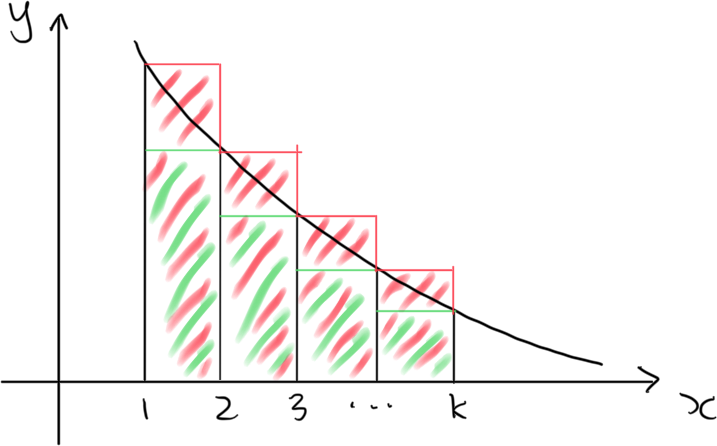
\includegraphics[scale=0.4]{fig/series-integral-test.png}
    \caption{Integral Test for Series}
    \label{fig:series-integral-test}
\end{figure}

\begin{proof}
    We refer to \autoref{fig:series-integral-test}. We first observe that
    \[
        s_k - a_1 = \sum_{n = 2}^{k} a_n = \textcolor{Green}{\sum A_{\text{green}}} \leq \int_{1}^{k} f\pqty{t} \dd{t}
    \]
    and
    \[
        s_{k - 1} = \sum_{n = 1}^{k - 1} a_n = \textcolor{Red}{\sum A_{\text{red}}} \geq \int_{1}^{k} f\pqty{t} \dd{t}.
    \]

    We observe that \(a_n \geq 0\) shows that \(s_k\) has to be increasing.

    \(\implies\). With the \textcolor{Red}{red inequality}, we have
    \[
        \int_{1}^{k} f\pqty{t} \dd{t} \leq s_{k - 1} \leq s.
    \]

    \(\pqty{s_k}\) is increasing and converges by assumption, which means the integral sequence
    \[
        \pqty{\int_{1}^{x} f\pqty{t} \dd{t}}_x
    \]
    is also increasing and bounded, which means it has a limit.

    \(\impliedby\). If the limit of the integral exists, then the integral sequence
    \[
        \pqty{\int_{1}^{x} f\pqty{t} \dd{t}}_x
    \]
    is bounded. Using the \textcolor{Green}{green inequality}, we have
    \[
        s_k \leq \int_{1}^{k} f\pqty{t} \dd{t} + a_1
    \]
    is also bounded. This shows that \(\pqty{s_k}\) converges, so the infinite series converges.

    For the final part, set
    \[
        b_k = \sum_{n = 1}^{k} a_n - \int_{1}^{k} f\pqty{x} \dd{x} = s_k - \int_{1}^{k} f\pqty{x} \dd{x},
    \]
    and hence we have
    \[
        b_k - b_{k - 1} = a_k - \int_{k - 1}^{k} f\pqty{t} \dd{t} = f\pqty{k} \cdot 1 - \int_{k - 1}^{k} f\pqty{t} \dd{t} \leq 0,
    \]
    which shows that this is a decreasing sequence. But also, from the \textcolor{Green}{green inequality}, we have \(b_k \geq a_k = f\pqty{k} \geq 0\), so \(\pqty{b_k}\) is bounded below. This means it has a limit \(l\).

    We know that \(l \in \ccintv{0}{a_1}\), because (re-using the \textcolor{Green}{green inequality})
    \[
        0 \leq f\pqty{k} \leq b_k \leq a_1 = f\pqty{1}
    \]
    and non-strict inequalities are preserved in the limit.
\end{proof}

\begin{examples}[Integral Test]
    \label{ex:integral-test}%
    \begin{itemize}
        \item For \(p > 0\), \(\sum n^{-p}\) converges if and only if \(p > 1\). First, \(f\pqty{t} = t^{-p}\) is decreasing and continuous on \(\cointv{1}{\plusinfty}\). We have
        \begin{align*}
            \lim_{n \to \infty} \int_{1}^{n} \frac{1}{t^p} \dd{t} &= \lim_{n \to \infty} \begin{cases}
                \bqty{\log t}_{1}^{n}, & p = 1, \\
                \bqty{\frac{1}{-p + 1} \cdot t^{-p + 1}}_{1}^{n}, & p \neq 1, \\
            \end{cases} \\
            &= \begin{cases}
                \plusinfty, & p = 1, \\
                0, & p \neq 1.
            \end{cases}
        \end{align*}

        In particular, this shows that the harmonic series diverges. But is there a `slower diverging series' than the harmonic series?

        \item We investigate \(\sum_{n = 2}^{\infty} \frac{1}{n \log n}\). Evaluating the integral gives
        \begin{align*}
            \int_{2}^{n} \frac{\dd{t}}{t \log t} &= \int_{\log 2}^{\log n} \frac{\dd{u}}{u} \\
            &= \bqty{\log u}_{\log 2}^{\log n} \\
            &= \log \log n - \log \log 2 \\
            &\to \plusinfty
        \end{align*}
        as \(n \to \infty\). By \autoref{prop:ser-test-integral} (Integral Test), this series diverges.

        \item The series \(\sum_{n = 2}^{\infty} \frac{1}{n \pqty{\log n}^2}\) converges by evaluating a similar integral.
    \end{itemize}
\end{examples}

Another useful result is the following, but the proof is non-examinable.

\begin{proposition}[Cauchy Condensation Test]
    \label{prop:ser-test-cauchy-condensation}%
    Let \(a_n \geq 0\) for all \(n \in \NN\), and let \(\pqty{a_n}\) be decreasing. Then \(\sum_{n = 1}^{\infty} a_n\) converges, if and only if the condensed series
    \[
        \sum_{n = 0}^{\infty} 2^n a_{2^n}
    \]
    converges.
\end{proposition}

\begin{proof}[\proofname\ using \autoref{prop:ser-test-integral} (Integral Test) (Non-Examinable)]
    Let \(a_n = f\pqty{n}\), and since \(a_n\) is positive and decreasing, we may choose \(f\) to be positive, decreasing and continuous. Note that
    \[
        \int_{1}^{2^x} f\pqty{t} \dd{t} = \log 2 \int_{0}^{x} 2^u f\pqty{2^u} \dd{u},
    \]
    by a change of variables \(t = 2^u\). Hence, applying \autoref{prop:ser-test-integral} (Integral test), we have
    \begin{align*}
        \sum_{n = 1}^{\infty} a_n \text{ converges} &\iff \lim_{x \to \infty} \sum_{n = 1}^{2^x} a_n \text{ exists} && \text{Partial Sums are Monotone}\\
        &\iff \lim_{x \to \infty} \int_{1}^{2^x} f\pqty{t} \dd{t} \text{ exists} \\
        &\iff \lim_{x \to \infty} \int_{0}^{x} 2^u f\pqty{2^u} \dd{u} \text{ exists.} && \text{Constant does not affect Convergence}
    \end{align*}

    Now, since \(f\) is decreasing, let \(g\pqty{t} = 2^t f\pqty{2^t}\), we have
    \[
        \forall t \in \ccintv{2^n}{2^{n + 1}}: f\pqty{2^n} \geq f\pqty{t} \geq f\pqty{2^{n + 1}},
    \]
    and hence
    \[
        \forall t \in \ccintv{n}{n + 1}: 2^{n + 1} f\pqty{2^n} \geq g\pqty{t} = 2^t f\pqty{2^t} \geq 2^n f\pqty{2^{n + 1}}.
    \]

    Integrating this in \(\ccintv{n}{n + 1}\) gives
    \[
        2^{n + 1} f\pqty{2^n} \geq \int_{n}^{n + 1} g\pqty{t} \dd{t} \geq 2^n f\pqty{2^{n + 1}},
    \]
    and hence summing this from \(n = 1\) to \(k\), we have
    \[
        2 \cdot \sum_{n = 1}^{k} 2^n f\pqty{2^n} \geq \int_{1}^{k + 1} g\pqty{t} \dd{t} \geq \frac{1}{2} \sum_{n = 1}^{k} 2^{n + 1} f\pqty{2^{n + 1}},
    \]
    and putting back \(a\)s gives us
    \[
        2 \cdot \sum_{n = 1}^{k} 2^n a_{2^n} \geq \int_{1}^{k + 1} g\pqty{t} \dd{t} \geq \frac{1}{2} \sum_{n = 1}^{k} 2^{n + 1} a_{2^{n + 1}},
    \]
    which means the sequence of the integrals and the series enforces bounds on  each other, giving equivalent convergence properties, and hence finishing our proof.
\end{proof}

\begin{proof}[\proofname\ considering Partial Sums (Non-Examinable)]
    Let the partial sums be
        \[
            A_m = \sum_{n = 1}^{m} a_n \qand B_k = \sum_{t = 0}^{k} 2^t \cdot a_{2^t}.
        \]

        Both \(\pqty{A_m}\) and \(\pqty{B_k}\) are increasing since \(\pqty{a_n}\) is non-negative. Therefore, convergence of \(\pqty{A_m}\) and \(\pqty{B_k}\) is equivalent to the convergence of some subsequence of them.

        We first show that for all \(k \geq 0\), that
        \[
            A_{2^{k + 1} - 1} \leq B_{k} \leq A_{2^k - 1} + A_{2^k}.
        \]

        For the left-hand side inequality, we have
        \begin{align*}
            B_k &= a_1 + \pqty{a_2 + a_2} + \pqty{a_4 + a_4 + a_4 + a_4} + \cdots + \pqty{a_{2^k} + \cdots + a_{2^k}} \\
            &\geq a_1 + \pqty{a_2 + a_3} + \pqty{a_4 + a_5 + a_6 + a_7} + \cdots + \pqty{a_{2^k} + \cdots + a_{2^{k + 1} - 1}} \\
            &= A_{2^{k + 1} - 1}.
        \end{align*}

        For the right-hand side inequality, we have
        \begin{align*}
            B_k &= a_1 + \pqty{a_2 + a_2} + \pqty{a_4 + a_4 + a_4 + a_4} + \cdots + \pqty{a_{2^k} + \cdots + a_{2^k}} \\
            &\leq a_1 + \pqty{a_1 + a_2} + \pqty{a_2 + a_3 + a_3 + a_4} + \cdots \\
            &\phantom{=} + \pqty{a_{2^{k - 1}} + a_{2^{k - 1} + 1} + a_{2^{k - 1} + 1} + \cdots  + a_{2^k - 1} + a_{2^k - 1} + a_{2^k}} \\
            &= \pqty{a_1 + a_1} + \pqty{a_2 + a_2} + \pqty{a_3 + a_3} + \cdots + \pqty{a_{2^k - 1} + a_{2^k - 1}} + a_{2^k} \\
            &= A_{2^k - 1} + A_{2^k}.
        \end{align*}

        With this inequality and that both partial sums are monotone, we may conclude that their convergence is equivalent.
\end{proof}

Next, we look at sequences with infinitely many terms that are negative.

\begin{proposition}[Alternating Series Test]
    \label{prop:ser-test-alternating}%
    Let \(\pqty{a_n}\) be a decreasing sequence with \(a_n \geq 0\), and \(a_n \to 0\). Then the sum
    \[
        \sum_{n = 1}^{\infty} \pqty{-1}^{n + 1} a_n
    \]  
    converges.
\end{proposition}

\autoref{fig:alternating-series-test} gives a good visualisation of the partial sums, and also some insights into the proof.

\begin{figure}[ht!]
    \center
    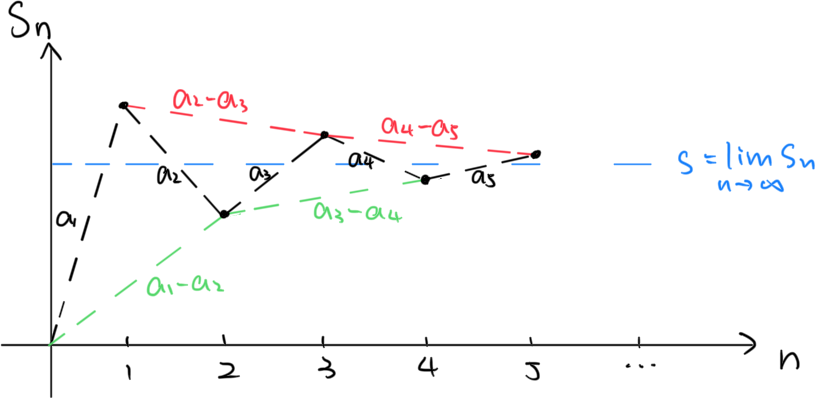
\includegraphics[scale=0.4]{fig/alternating-series-test.png}
    \caption{Alternating Series Test}
    \label{fig:alternating-series-test}
\end{figure}

\begin{example}[Alternating Harmonic Series]
    \label{ex:alternating-harmonic}%
    \autoref{prop:ser-test-alternating} (Alternating Series Test) tells us that
    \[
        \sum_{n = 1}^{\infty} \frac{\pqty{-1}^{n + 1}}{n}
    \]
    converges (to \(\log 2\)), while the harmonic series \(\sum_{n = 1}^{\infty} \frac{1}{n}\) diverges.
\end{example}

\begin{proof}[\proofname\ of \autoref{prop:ser-test-alternating} (Alternating Series Test)]
    We look at the sequence of partial sums
    \[
        s_k = \sum_{n = 1}^{k} \pqty{-1}^{n + 1} a_n.
    \]
    
    Then we have
    \[
        s_{2k} = \pqty{a_1 - a_2} + \pqty{a_3 - a_4} + \cdots + \pqty{a_{2k - 1} - a_{2k}},
    \]
    and since everything in the brackets are non-negative, we have
    \[
        s_2 \leq s_4 \leq s_6 \leq \cdots
    \]
    which says \(\pqty{s_{2k}}_{k \in \NN}\) is increasing.

    Similarly, for the odd-indexed terms,
    \[
        s_{2k + 1} = a_1 + \pqty{- a_2 + a_3} + \pqty{- a_4 + a_5} + \cdots + \pqty{- a_{2k} + a_{2k + 1}}
    \]
    and since everything in the brackets are non-positive, we have
    \[
        s_1 \geq s_3 \geq s_5 \geq \cdots
    \]
    which says \(\pqty{s_{2k - 1}}_{k \in \NN}\) is decreasing.

    Also, we notice that \(s_{2k + 1} - s_{2k} = a_{2k + 1} > 0\), and hence,
    \[
        a_1 - a_2 = s_2 \leq s_{2k} \leq s_{2k + 1} \leq s_1 = a_1,
    \]
    i.e., \(s_1\) imposes an upper bound on \(\pqty{s_{2k}}_{k \in \NN}\), and \(s_2\) imposes a lower bound on \(\pqty{s_{2k - 1}}_{k \in \NN}\).
    
    Applying \autoref{thm:monotone-convergence} (Monotone Convergence Theorem) to the two subsequences gives that
    \[
        s_{2k} \to s \qand s_{2k - 1} \to s'
    \]
    for \(s, s' \in \RR\). We would like to show \(s = s'\).

    But note that \(s_{2k + 1} - s_{2k} = a_{2k + 1} \to 0\), and \(s_{2k + 1} - s_{2k} \to s - s'\), so \(s = s'\). This means the odd and even indexed subsequence of \(\pqty{s_k}_{k \in \NN}\) converges to the same limit.

    Finally, if the odd-indexed and even-indexed subsequence converges to the same limit, then the sequence must also converge to that limit. Indeed, if both subsequences converge to the limit, say \(s\), then there is some \(N_1\pqty{\epsilon}\) and \(N_2\pqty{\epsilon}\) for \(\epsilon > 0\), such that
    \[
        \forall n \geq N_1: \abs{s_{2k} - s} < \epsilon \qand \forall n \geq N_2: \abs{s_{2k + 1} - s} < \epsilon.
    \]

    Therefore, let \(N\pqty{\epsilon} = \max\Bqty{2 N_1\pqty{\epsilon}, 2 N_2 \pqty{\epsilon} + 1}\), then for all \(n \geq N\), we have \(n \geq 2 N_1\) and \(n \geq 2 N_2 + 1\), so
    \[
        \abs{s_n - s} < \epsilon
    \]
    showing convergence indeed.
\end{proof}

We now study the idea of `signs' in the series.

\begin{definition}[Absolute Convergence]
    \label{def:ser-absolute-convergence}%
    We say the series \(\sum a_n\) is \term{absolutely convergent} if \(\sum \abs{a_n}\) converges.
\end{definition}

\begin{remark}
    Since \(\abs{a_n} \geq 0\) for all \(n \in \NN\), \autoref{prop:ser-test-comparison} (Comparison Test), \autoref{prop:ser-test-root} (Root Test), \autoref{prop:ser-test-ratio} (Ratio Test), \autoref{prop:ser-test-integral} (Integral Test) and \autoref{prop:ser-test-cauchy-condensation} (Cauchy Condensation Test) are good tests on absolute convergence.
\end{remark}

But why do we even bother studying absolute convergence -- what is its relation with simply `convergence'?

\begin{theorem}[Absolute Convergence implies Convergence]
    \label{thm:ser-absolute-convergence-implies-convergence}%
    Absolute convergence implies convergence.
\end{theorem}

\begin{remark}
    The converse is false by examining \autoref{ex:alternating-harmonic} (Alternating Harmonic Series).
\end{remark}

\begin{proof}
    Let \(s_k = \sum_{n = 1}^{k} a_n\) and \(r_k = \sum_{n = 1}^{k} \abs{a_n}\). Since \(\pqty{r_k}\) converges, it is Cauchy, and to show \(\pqty{s_k}\) converges, we want to show that it is Cauchy.

    Note that
    \begin{align*}
        \abs{s_k - s_l} &= \abs{\sum_{n = l - 1}^{k} a_n} \\
        &\leq \sum_{n = l - 1}^{k} \abs{a_n} \\
        &= r_k - r_l
    \end{align*}
    which shows that \(\pqty{r_k}\) is Cauchy implies that \(\pqty{s_k}\) is Cauchy. This finishes the proof.
\end{proof}

\begin{proof}[\proofname\ for the Real Case]
    We have
    \[
        0 \leq a_n + \abs{a_n} \leq 2 \abs{a_n}
    \]
    and the result follows from \autoref{prop:ser-test-comparison} (Comparison Test).
\end{proof}

This means that absolute convergent series is strictly a subset of convergent series. We give a name for the series which converges but not absolutely as well.

\begin{definition}[Conditional Convergence]
    \label{def:ser-conditional-convergence}%
    A series that is convergent but is not absolutely convergent is \term{conditional convergent}.
\end{definition}

Conditionally convergent sequences have a very different style to absolutely convergent sequences, in the sense that they `behave weirdly'. In particular, we cannot do the following to a conditionally convergent series (but we can to an absolutely convergent one).

\begin{itemize}
    \item Rearrange Terms (c.f. \autoref{prop:ser-rearrangement-absolute-convergence} and Riemann Series/Rearrangement Theorem);
    \item Multiply series to a Convergent Product Series;
    \item Put Brackets on Terms (i.e. only studying a subsequence of partial sums).
\end{itemize}

\begin{example}[Rearranging the Alternating Harmonic Series]
    \label{ex:ser-rearrange-alternating-harmonic}%
    We look at the alternating harmonic series.

    \[
        \sum_{n = 1}^{\infty} \frac{\pqty{-1}^{n + 1}}{n} = 1 - \frac{1}{2} + \frac{1}{3} - \frac{1}{4} + \frac{1}{5} - \frac{1}{6} + \cdots.
    \]

    Rearranging terms on the right gives
    \begin{align*}
        &\phantom{=} \pqty{1 - \frac{1}{2}} - \frac{1}{4} + \pqty{\frac{1}{3} - \frac{1}{6}} - \frac{1}{8} + \pqty{\frac{1}{5} - \frac{1}{10}} - \frac{1}{12} + \pqty{\frac{1}{7} - \frac{1}{14}} + \cdots \\
        &= \frac{1}{2} - \frac{1}{4} + \frac{1}{6} - \frac{1}{8} + \frac{1}{10} - \frac{1}{12} + \frac{1}{14} + \cdots \\
        &= \frac{1}{2} \pqty{1 - \frac{1}{2} + \frac{1}{3} - \frac{1}{4} + \frac{1}{5} - \frac{1}{6} + \cdots} \\
        &= \frac{1}{2} \sum_{n = 1}^{\infty} \frac{\pqty{-1}^{n + 1}}{n}.
    \end{align*}

    We may conclude that
    \[
        \sum_{n = 1}^{\infty} \frac{\pqty{-1}^{n + 1}}{n} = \frac{1}{2}  \sum_{n = 1}^{\infty} \frac{\pqty{-1}^{n + 1}}{n}
    \]
    which is nonsense. The non-trivial part of this manipulation is the rearrangement part -- the order of the elements in the sum matters. (This is not the case for absolutely convergent series, which are much better behaved!)
\end{example}

\begin{proposition}[Rearrangement under Absolute Convergence]
    \label{prop:ser-rearrangement-absolute-convergence}%
    Let \(\functiondomain{\sigma}{\NN}{\NN}\) be a bijection, and let \(\pqty{a_n}\) be absolutely convergent. Then the rearranged series given by terms \(a_n' = a_{\sigma\pqty{n}}\) is absolutely convergent, and converges to the same limit.
\end{proposition}

\begin{proof}
    We let \(s_k = \sum_{n = 1}^{k} a_n\), and we know that \(s_k \to s\) as \(k \to \infty\) for some \(s \in \RR\).

    This means that for all \(\epsilon > 0\), there is some \(N = N\pqty{\epsilon}\), such that
    \[
        \forall n \geq N: \abs{s_k - s} < \epsilon
    \]
    and that the remaining terms (since it absolutely converges)
    \[
        \sum_{k = N}^{\infty} \abs{a_n} < \epsilon.
    \]

    There must exist some \(N_1 \geq N\), such that \(a_1, \ldots, a_N\) are included in \(a'1, \ldots, a'_{N_1}\). (Formally, this means there is some \(N_1 \geq N\), such that for all \(1 \leq n \leq N\), we have \(\sigma\pqty{n} \leq N_1\).)

    Hence, for \(m \geq N_1\), we have
    \[
        \sum_{n = 1}^{m} a_n' = \sum_{n = 1}^{N} a_n + \pqty{\pqty{m - N} \text{ terms of }\pqty{a_n}\text{ sequence with index}\geq N}.
    \]

    Hence,
    \[
        \abs{\sum_{n = 1}^{m} a_n' - s} \leq \abs{s_N - s} + \sum_{k = N}^{\infty} \abs{a_n} \leq 2\epsilon
    \]
    where the second sum above is a `huge' overestimate of the \(\pqty{m - N}\) terms, (but guaranteed to be small), showing that the partial sums of the rearranged series converges to the value of the sum of the original series.
\end{proof}

Now, we introduce the final test.

\begin{proposition}[Dirichlet's Test]
    \label{prop:ser-test-dirichlet}%
    Let \(\pqty{a_n}\) be a sequence (real or complex) with bounded partial sums (i.e. the partial sums form a bounded sequence), and \(\pqty{b_n}\) be a positive, decreasing sequence of reals, and \(b_n \to 0\) as \(n \to \infty\). Then the product series
    \[
        \sum_{n = 1}^{\infty} a_n b_n
    \]
    converges.
\end{proposition}

We introduce a useful lemma which is similar to integration by parts, and is indeed named similarly.

\begin{lemma}[Summation by Parts]
    \label{lem:ser-summation-by-parts}%
    Let \(\pqty{a_n}, \pqty{b_n}\) be two sequences, and let
    \[
        S_n = \sum_{i = 1}^{n} a_n
    \]
    be the partial sums of \(a_n\), with the convention that \(S_0 = 0\). Then we have
    \[
        \sum_{j = m}^{n} a_j b_j = S_n b_n - S_{m - 1} b_m + \sum_{j = m}^{n - 1} S_j \pqty{b_j - b_{j + 1}}.
    \]
\end{lemma}

\begin{proof}
    For any \(1 \leq m \leq n\), we have
    \begin{align*}
        \text{Right-Hand Side} &= \sum_{j = m}^{n} S_j b_j - \sum_{j = m - 1}^{n - 1} S_j b_{j + 1} \\
        &= \sum_{j = m}^{n} S_j b_j - \sum_{j = m}^{n} S_{j - 1} b_j \\
        &= \sum_{j = m}^{n} \pqty{S_j - S_{j - 1}} b_j \\
        &= \sum_{j = m}^{n} a_j b_j \\
        &= \text{Left-Hand Side}
    \end{align*}
    as desired.
\end{proof}

\begin{proof}[\proofname\ using \autoref{thm:ser-absolute-convergence-implies-convergence} (Absolute Convergence)]
    We apply the \autoref{lem:ser-summation-by-parts} for \(m = 1\), which gives
    \[
        \sum_{j = 1}^{n} a_j b_j = S_n b_n + \sum_{j = 1}^{n - 1} S_j \pqty{b_j - b_{j + 1}}.
    \]

    Let \(M\) be a bound of \(S_n\), so \(\abs{S_n} \leq M\) for all \(n \in \NN\). Therefore,
    \[
        0 \leq \abs{S_n b_n} \leq M b_n
    \]
    and hence \(S_n b_n \to 0\).

    Furthermore,
    \begin{align*}
        \sum_{j = 1}^{n - 1} \abs{S_j \pqty{b_j - b_{j + 1}}} &= \sum_{j = 1}^{n - 1} \abs{S_j} \pqty{b_j - b_{j + 1}} \\
        &\leq M \sum_{j = 1}^{n - 1} \pqty{b_j - b_{j + 1}} \\
        &= M \pqty{b_1 - b_n}.
    \end{align*}

    As \(n \to \infty\), the right-hand side converges to \(M b_1\), imposing an upper bound on the partial absolute sums. Therefore, by \autoref{thm:ser-absolute-convergence-implies-convergence} (Absolute Convergence implies Convergence), the sum
    \[
        \sum_{j = 1}^{\infty} S_j \pqty{b_j - b_{j + 1}}
    \]
    converges. Hence, \(\sum_{j = 1}^{\infty} a_j b_j\) converges.
\end{proof}

\begin{proof}[\proofname\ using \autoref{thm:completeness-of-r-and-c} (Cauchy Sequences Converge)]
    Similarly, since \(S_n\) is bounded, let \(\abs{S_n} \leq M\) for all \(n \in \NN\). Then, using \autoref{lem:ser-summation-by-parts} (Summation by Parts),
    \begin{align*}
        \abs{\sum_{j = m}^{n} a_j b_j} &\leq M b_n + M b_m + \sum_{j = m}^{n - 1} M \pqty{b_j - b_{j + 1}} \\
        &\leq M \bqty{b_n + b_m + \sum_{j = m}^{n - 1} \pqty{b_j - b_{j + 1}}} \\
        &= M \bqty{b_n + b_m + \pqty{b_m - b_n}} \\
        &= 2 M b_m.
    \end{align*}

    Let \(\epsilon > 0\) be arbitrary. Since \(b_n \to 0\), we let \(N \in \NN\) be such that \(\abs{b_n} < \frac{\epsilon}{2M}\) for all \(n \geq N\).
    
    Then, for all \(N \leq m \leq n\), we have
    \[
        \abs{\sum_{j = m}^{n} a_j b_j} \leq 2 M b_m < \epsilon
    \]
    and this shows that the partial sums of \(a_j b_j\) is Cauchy, hence convergent.
\end{proof}

Another result we have is that there is `no slowest divergent series'.

\begin{lemma}[No Slowest Divergent Series]
    \label{lem:no-slowest-divergent-series}%
    Suppose that \(\sum a_n\) diverges to infinity and \(a_n > 0\). Then there is a sequence \(\pqty{b_n}\) with \(\frac{b_n}{a_n} \to 0\) and \(\sum b_n\) divergent.
\end{lemma}

\begin{proof}
        We let the partial sums of \(\pqty{a_n}\) be
    \[
        S_n = \sum_{m = 1}^{n} a_m,
    \]
    and we construct the sequence
    \[
        b_n = \frac{a_n}{S_n}.
    \]

    We must have
    \[
        \frac{b_n}{a_n} = \frac{1}{S_n} \to 0.
    \]

    Let the partial sums of \(b_n\) be
    \[
        S'_n = \sum_{m = 1}^{n} b_m.
    \]

    To show the infinite series of \(b_n\) diverges, we show that \(S'_n\) is not Cauchy. Indeed, for any \(m_1, m_2 \in \NN\), where \(m_1 > m_2\), we have
    \begin{align*}
        S'_{m_1} - S'_{m_2} &= \sum_{n = m_2}^{m_1} b_n \\
        &= \sum_{n = m_2}^{m_1} \frac{a_n}{S_n} \\
        &> \frac{1}{S_{m_1}} \sum_{n = m_2}^{m_1} a_n \\
        &= \frac{S_{m_1} - S_{m_2}}{S_{m_1}} \\
        &= 1 - \frac{S_{m_2}}{S_{m_1}},
    \end{align*}
    which shows for all \(m, n \in \NN\), \(m > n\), we have
    \[
        S'_{m} - S'_{n} > 1 - \frac{S_n}{S_m}.
    \]

    To show that \(S'_n\) is not Cauchy, we want to show that
    \[
        \exists \epsilon > 0, \forall N \in \NN, \exists m, n \geq N : \abs{S'_m - S'_n} \geq \epsilon.
    \]

    We let \(0 < \epsilon < 1\), say \(\epsilon = \frac{1}{2}\), so \(1 - \epsilon > 0\). Let \(N \in \NN\) be arbitrary, and let \(n = N\). We have
    \[
        1 - \frac{S_n}{S_m} \geq \epsilon \iff \frac{S_n}{S_m} \leq 1 - \epsilon \iff S_m \geq \frac{S_n}{1 - \epsilon}.
    \]

    Note that \(n = N\) is fixed, so the right-hand side is a constant. Since the sequence \(\pqty{S_m}\) is positive and diverges to infinity, the terms can be arbitrarily large however large \(m\) is, and in particular it can be larger than \(\frac{S_n}{1 - \epsilon}\), for some \(m > N\). This provides a diverging lower bound for \(\pqty{S'_n}\), finishing our proof on \(S'_n\) is divergent, and hence \(\sum b_n\) is divergent.
\end{proof}

\begin{proposition}[Convergence of Product Series]
    If both \(\sum a_n\) and \(\sum b_n\) both converges absolutely, then \(\sum a_n b_n\) converges absolutely.
\end{proposition}

\begin{remark}
    This is not true for non-absolute convergent series, with the following counterexample. Let \(a_n = b_n = \pqty{-1}^{n + 1} \frac{1}{\sqrt{n}}\). By \autoref{prop:ser-test-alternating} (Alternating Series Test), since \(\frac{1}{\sqrt{n}} \to 0\) and is decreasing, \(\sum a_n\) and \(\sum b_n\) both converge.

    But \(a_n b_n = \frac{1}{n}\) and \(\sum a_n b_n\) is the harmonic series, which diverges.
\end{remark}

\begin{proof}[\proofname\ using Bounds]
    Since \(\sum a_n\) converges, \(a_n\) is bounded, say \(a_n \leq M\) for all \(n\). Then,
    \[
            0 \leq \abs{a_n b_n} \leq M \abs{b_n}
    \]

    So by \autoref{prop:ser-test-comparison} (Comparison Test), the product series \(a_n b_n\) converges absolutely.
\end{proof}

\begin{remark}
    Note we only used the condition that \(a_n\) is bounded here, so the conditions can be weakened.
\end{remark}

\begin{proof}[\proofname\ using Cauchy--Schwarz]
    Without loss of generality, we take \(a_n, b_n \geq 0\) (by taking the moduli of the terms).

    Since \(\sum a_n\) and \(\sum b_n\) converge absolutely, we have \(\sum a_n^2\) and \(\sum b_n^2\) converge absolutely. Hence,
    \[
        \pqty{\sum_{n = 1}^{m} \pqty{a_n b_n}}^2 \leq \pqty{\sum_{n = 1}^{m} a_n^2} \cdot \pqty{\sum_{n = 1}^{m} b_n^2}
    \]
    and therefore the partial sums of the product series are bounded above. Since the partial sums are increasing, they converge.
\end{proof}
\begin{remark}
    The conditions for this can be weakened -- for example using H\"older's inequality, a more general version of Cauchy--Schwarz.
\end{remark}
\section{Continuity of Functions}
\subsection{Limits of Functions}

Take \(\functiondomain{f}{X}{\CC}\) for some \(X \subseteq \CC\). We want to define what we mean by \(f\pqty{z} \to y\) as \(z \to a\), \emph{even if \(a \notin X\)}.

\begin{figure}[ht!]
    \centering
    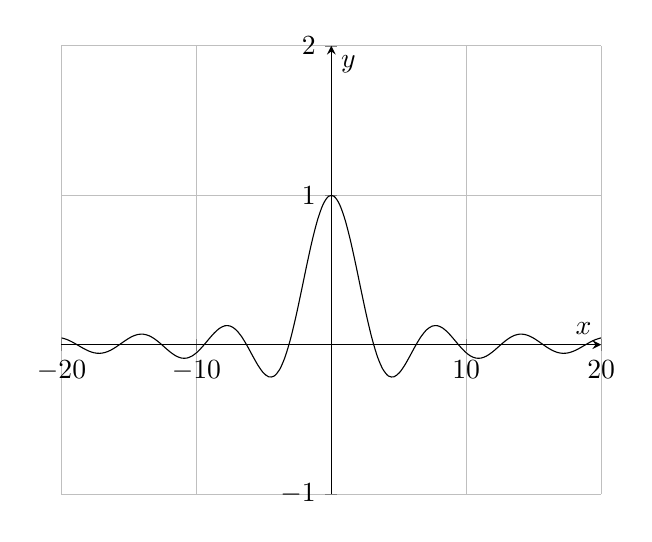
\begin{tikzpicture}[scale=1]
        \begin{axis}[grid=both,
                     xmin=-20, xmax=20, xlabel=\(x\),
                     ymin=-1, ymax=2, ylabel=\(y\),
                    axis lines=center, >=stealth]
        \addplot[domain=-20:20, samples=100] plot[smooth] {sin(deg(x))/x};
        \end{axis}
    \end{tikzpicture}
    \caption{Graph of \(\frac{\sin x}{x}\)}
    \label{fig:graph-sin-x-x}
\end{figure}

\begin{example}[The Function \(\frac{\sin x}{x}\)]
    The function \(f\pqty{x} = \frac{\sin x}{x}\) is not defined at \(x = 0\). But from \autoref{fig:graph-sin-x-x}, we are very tempted to say that this function has a limit of \(1\) as the function tends to \(0\), and if so, we may extend the domain for a new function, to include \(x = 0\) to take a value of \(1\), e.g.,
    \[
        f\pqty{x} = \begin{cases}
            \frac{\sin x}{x}, & x \neq 0, \\
            \lim_{x \to 0} \frac{\sin x}{x}, & x = 0.
        \end{cases}
    \]
\end{example}

The reason why we can hope to make sense of \(\lim_{x \to 0} \frac{\sin x}{x}\) is that there are points in the domain that are very close to \(0\), and we could use points ever closer to \(0\) to determine the value of that `limit'.

In other words, \(0\) is an \term{accumulation point} for \(\RR \setminus \set{0}\): for any threshold \(\delta > 0\), we can always find \(x \in \RR \setminus \set{0}\), such that \(\abs{x - 0} < \delta\).

\begin{definition}[Accumulation and Isolated Point]
    \label{def:fn-accumulation-isolated-point}%
    Let \(X \subseteq \CC\) and \(a \in \CC\). We say \(a\) is an \term{accumulation point} for \(X\), if that
    \[
        \forall \delta > 0, \exists z \in X \setminus \set{a}: \abs{z - a} < \delta.
    \]

    If \(a \in X\) and it is not an accumulation point, then we say \(a\) is \term{isolated}.
\end{definition}

\begin{example}[Accumulation and Isolated Point]
    \label{ex:fn-accumulation-isolated-point}%
    \begin{itemize}
        \item The set \(X = \set{0} \cup \ccintv{1}{2}\) has \(0\) as an isolated point. On the other hand, all points in \(\ccintv{1}{2}\) are accumulation points for \(X\).
        \item The points on the unit circle \(S = \set{z \in \CC}{\abs{z} = 1}\) are accumulation points for \(D = \set{z \in \CC}{\abs{z} < 1}\). Also, all the points in \(D\) are also accumulation points for \(D\). \autoref{fig:accumulation-point-c} demonstrates this example.
        \item If we look at \(\set{z \in \CC}{\abs{z} \leq 1}\), then all the points in this set are accumulation points. 
    \end{itemize}
\end{example}

\begin{figure}[ht!]
    \centering
    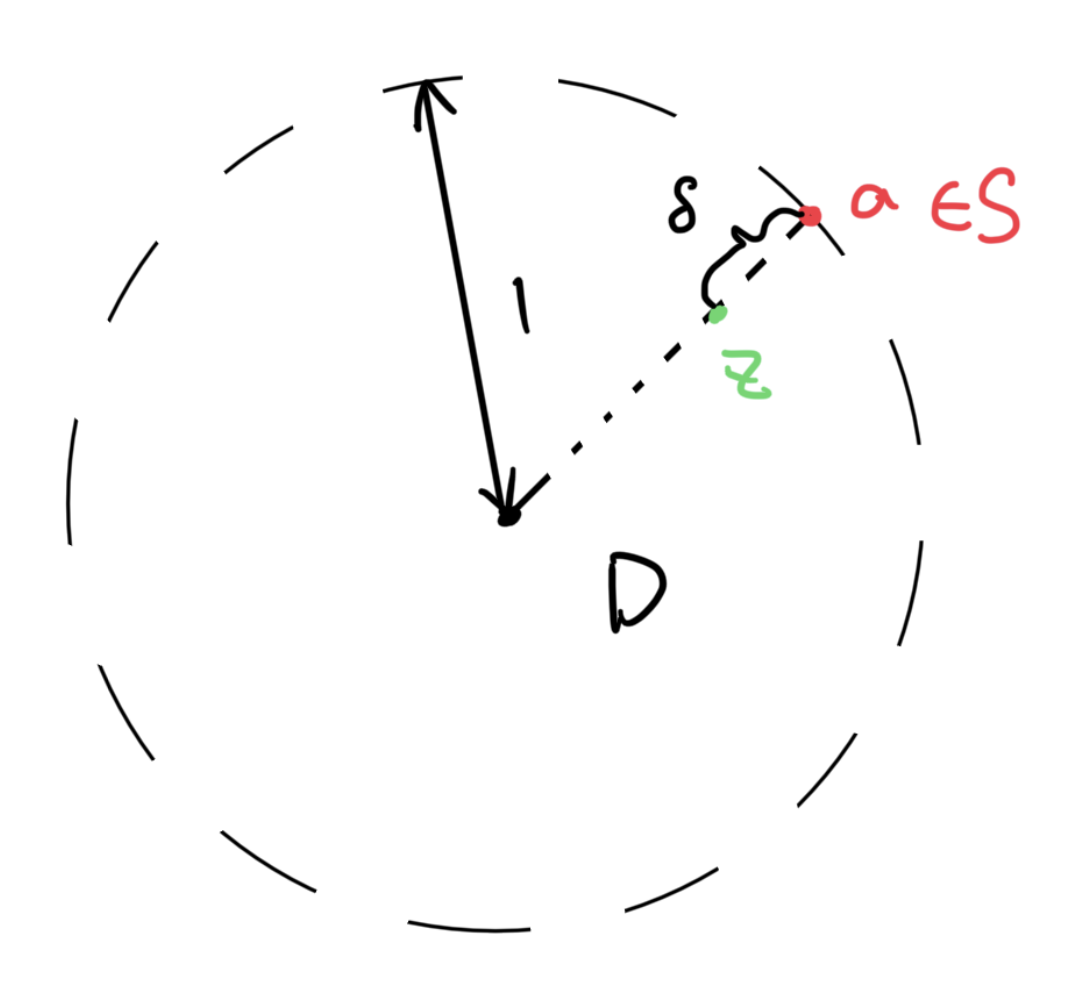
\includegraphics[scale=0.3]{fig/accumulation-points.png}
    \caption{Accumulation Points on Complex Unit Circle}
    \label{fig:accumulation-point-c}
\end{figure}

\begin{lemma}[Accumulation Points are Limit Points]
    Let \(X \subseteq \CC\) and \(a \in \CC\). Then \(a\) is an accumulation point for \(X\) if and only if there exists \(\pqty{x_n}\) in \(X \setminus \set{a}\), such that \(\lim_{n \to \infty} x_n = a\).
\end{lemma}

\begin{proof}
    If there is some \(\pqty{x_n} \subseteq X \setminus \set{a}\) with \(x_n \to a\), then by definition,
    \[
        \forall \epsilon > 0, \exists N = N\pqty{\epsilon} \in \NN, \forall n \geq N: \abs{x_n - a} < \delta.
    \]

    Now, let \(\delta > 0\) be arbitrary, then take \(N = N\pqty{\delta}\), therefore we have \(x_N \in X \setminus \set{a}\) with \(\abs{x_N - a} < \delta\), showing that \(a\) is indeed an accumulation point.

    Conversely, given \(a\) is an accumulation point of \(X\), this means
    \[
        \forall \delta > 0, \exists z = z\pqty{\delta} \in X \setminus \set{a}: \abs{z - a} < \delta.
    \]

    Now, let \(x_n = z\pqty{\frac{1}{n}}\) for \(n \in \NN\), then \(x_n\) is indeed a sequence of \(X \setminus \set{a}\). Therefore,
    \[
        0 < \abs{x_n - a} = \abs{z\pqty{\frac{1}{n}} - a} \leq \frac{1}{n}
    \]
    and by the sandwich theorem, \(\abs{x_n - a} \to 0\), so \(x_n \to a\), as desired.
\end{proof}

Now we return to the definition of a limit. From the point we just saw, we want \(a\) to be an accumulation point of \(X\), since otherwise the behaviour of \(f\) as \(z\) `approaches' \(a\) itself does not make sense -- we need a path for \(z\) to approach the point, via its domain! 

We make sense of \(f\pqty{z}\) as \(z \to a\) by looking at points near \(a\). The idea is, no matter how small the threshold \(\epsilon > 0\), we may let the function be arbitrarily close to \(y\), as long as \(z\) is sufficiently close to \(a\). Formally, we want to define this as follows.

\begin{definition}[Limit of a Function]
    \label{def:fn-limit}%
    Let \(\functiondomain{f}{X \subseteq \CC}{\CC}\). We take some \(a \in \CC\) which is an accumulation point of \(X\).


    We say \(f\) \term{tends to} \(y \in \CC\) as \(z\) tends to \(a\), if
    \[
        \forall \epsilon > 0, \exists \delta = \delta \pqty{\epsilon} > 0, \forall 0 < \abs{z - a} < \delta, z \in X: \abs{f\pqty{z} - y} < \epsilon,
    \]
    and we denote this as \(f\pqty{z} \to y\) as \(z \to a\), or \(\lim_{z \to a} f\pqty{z} = y\).

    Similarly, we say \(f\) diverges to \(\infty\) as \(z \to a\), if
    \[
        \forall L > 0, \exists \delta = \delta\pqty{L} > 0, \forall 0 < \abs{z - a} < \delta, z \in X: \abs{f\pqty{z}} > L.
    \]
\end{definition}

\begin{remark}
    \begin{itemize}
        \item We shall not worry about the limit at an isolated point, since there is not a good behaviour of `approaching' \(a\) in any sense. (Indeed, most of the following results on limits only concerns accumulation points.) Therefore, some choose to not define the limit at an isolated point, while others might choose to define \(\lim_{z \to a} f\pqty{z} = f\pqty{a}\). The latter might be chosen since it would make the limit condition for \autoref{def:fn-continuity} (Continuity) work for isolated points as well.
        
        In particular, our definition does not work well for isolated points, since for sufficiently small \(\delta\), there is no \(z \in X\) such that \(0 < \abs{z - a} < \delta\), and our condition is trivially true for \emph{any} \(y\) which is not what we want.

        \item Note that \(f\) may diverge to infinity at \(a \in \CC\), even with \(a \in X\). Consider the example
        \[
            f\pqty{x} = \begin{cases}
                \frac{1}{x^2}, & x \neq 0, \\
                0, & x = 0,
            \end{cases}  
        \]
        and at \(x = 0\), \(f\pqty{0} = 0\) but
        \[
            \lim_{x \to 0} f\pqty{x} \to \infty.
        \]
    \end{itemize}
\end{remark}

\begin{example}[\(\frac{\sin x}{x}\) as \(x \to 0\)]
    \label{ex:sin-x-x-limit}%
    We claim that \(\frac{\sin x}{x} \to 1\) as \(x \to 0\). Using trigonometry, we have that
    \[
        \cos x < \frac{\sin x}{x} < 1
    \]
    for all \(x \in \oointv{0}{\frac{\pi}{2}}\). Hence,
    \[
        \abs{\frac{\sin x}{x} - 1} < 1 - \cos x = 2 \sin^2 \pqty{\frac{x}{2}} < \frac{x^2}{2}.
    \]

    Hence, for all \(\epsilon > 0\), we choose \(\delta\pqty{\epsilon} = \sqrt{2\epsilon}\), and hence
    \[
        \abs{x - 0} < \delta \implies \abs{\frac{\sin x}{x} - 1} < \frac{\pqty{\sqrt{2 \epsilon}}^2}{2} = \epsilon
    \]
    for \(x > 0\), and since this function is even, the same behaviour holds for \(x < 0\), which finishes our proof.
\end{example}

\begin{lemma}[Sequential Limits / Heine's Theorem]
    \label{lem:fn-sequential-limits}%
    Let \(\functiondomain{f}{X \subseteq \CC}{\CC}\), and let \(a \in \CC\) be an accumulation point of \(X\). Then
    \[
        \lim_{z \to a} f\pqty{z} = y
    \]
    if and only if
    \[
        \lim_{n \to \infty} f\pqty{z_n} = y
    \]
    for any \(\pqty{z_n}\) on \(X \setminus \set{a}\), with \(z_n \to a\).

    Similarly, \(f\pqty{z}\) diverges to infinity, if and only if \(\pqty{f\pqty{z_n}}\) diverges to infinity for every \(\pqty{z_n}\) on \(X \setminus \set{a}\), with \(z_n \to a\).
\end{lemma}

\begin{proof}
    We prove for convergence, and the case for divergence is similar.
    
    Suppose that \(\lim_{z \to a} f\pqty{z} = y\). Let \(\epsilon > 0\) be arbitrary, and let \(\delta > 0\) be such that
    \[
        \forall z \in X, 0 < \abs{z - a} < \delta: \abs{f\pqty{z} - y} < \epsilon.
    \]

    Now, take any \(\pqty{z_n} \to a\) on \(X \setminus \set{a}\). Since \(\delta > 0\), there is some \(N > 0\) such that
    \[
        \forall n \geq N: 0 < \abs{z_n - a} < \delta.
    \]

    Hence,
    \[
        \forall n \geq N: \abs{f\pqty{z_n} - y} < \epsilon
    \]
    showing that the limit of the sequence converges as desired.

    Conversely, we prove using the contrapositive, so suppose \(\lim_{z \to a} f\pqty{z} \neq y\). Then for some \(\epsilon > 0\), we have for all \(\delta > 0\), we have
    \[
        \exists z \in X, 0 < \abs{z - a} < \delta: \abs{f\pqty{z} - y} \geq \epsilon.
    \]

    Taking \(\delta = 1, \frac{1}{2}, \frac{1}{3}, \ldots\), we construct a sequence of such \(z_n \in X\), and we have for all \(n \in \NN\),
    \[
        z_n \in X \qand 0 < \abs{z_n - a} < \frac{1}{n}
    \]
    which shows \(\pqty{z_n} \to a\) on \(X \setminus \set{a}\), and indeed,
    \[
        \abs{f\pqty{z_n} - y} \geq \epsilon,
    \]
    which shows that \(f\pqty{z_n} \notto y\). This finishes the proof.
\end{proof}

\begin{lemma}[Limit of Function is Unique]
    \label{lem:fn-limit-unique}%
    If \(\functiondomain{f}{X \subseteq \CC}{\CC}\) has a limit at \(a \in \CC\), then this limit is unique.
\end{lemma}

\begin{proof}[\proofname\ using Sequences]
    This is a corollary of \autoref{lem:fn-sequential-limits} due to the uniqueness of the limit of a sequence.
\end{proof}

\begin{proof}[\proofname\ using \(\epsilon-\delta\)]
    Suppose that \(f\pqty{z} \to y\) and \(f\pqty{z} \to x\) as \(z \to a\). We have that
    \[
        \abs{x - y} \leq \abs{x - f\pqty{z}} + \abs{f\pqty{z} - y}
    \]
    and using similar techniques in \autoref{lem:seq-limit-unique} (Sequences have Unique Limit), we have \(x = y\).
\end{proof}

\begin{lemma}[Function Limits Preserve Arithmetic]
    \label{lem:fn-limits-preserve-arithmetic}%
    Let \(\functiondomain{f, g}{X \subseteq \CC}{\CC}\), and \(a \in \CC\) be an accumulation point of \(X\). Suppose \(\lim_{z \to a} f\pqty{z} = a\) and \(\lim_{z \to a} g\pqty{z} = b\), then
    \begin{align*}
        \lim_{z \to a} \pqty{f\pqty{z} + g\pqty{z}} &= a + b, \\
        \lim_{z \to a} \pqty{f\pqty{z} \cdot g\pqty{z}} & = ab.
    \end{align*}

    Furthermore, if \(b \neq 0\), we have
    \[
        \lim_{z \to a} \frac{f\pqty{z}}{g\pqty{z}} = \frac{a}{b}.
    \]
\end{lemma}

\begin{proof}
    The techniques in proving this is similar to what we did in \autoref{lem:seq-limits-arithmetic} (Limit of Sequence Preserve Arithmetic), so we will not repeat the proof here.
\end{proof}

\subsection{Continuity of Functions}

\begin{definition}[Continuity]
    \label{def:fn-continuity}%
    Let \(\functiondomain{f}{X \subseteq \CC}{\CC}\).

    We say \(f\) is \term{continuous at some point \(a \in X\)}, if
    \[
        \forall \epsilon > 0, \exists \delta = \delta\pqty{\epsilon}, \forall \abs{z - a} < \delta, z \in X: \abs{f\pqty{z} - f\pqty{a}} < \epsilon.
    \]

    
    
    We say \(f\) is \term{continuous} if it is continuous at every point in \(X\).    
\end{definition}

\begin{remark}
    If \(a \in X\) is an isolated point, \(f\) is then trivially continuous at \(a\), because for sufficiently small \(\delta\), \(\abs{z - a} < \delta\) implies \(z = a\), so \(f\pqty{z} = f\pqty{a}\).

    On the other hand, if \(a \in X\) is an accumulation point, this is equivalent to saying
    \[
        \lim_{z \to a} f\pqty{z} = f\pqty{a}.
    \] 
\end{remark}

\begin{example}[Examples on Continuity]
    \label{ex:fn-continuity}
    \begin{itemize}
        \item \(f\pqty{z} = z\) is the identity function. This is continuous everywhere on the domain, say \(\CC\). For all \(\epsilon > 0\), we choose \(\delta = \epsilon\), so for all \(\abs{z - a} < \delta\), we have \(\abs{f\pqty{z} - f\pqty{a}} = \abs{z - a} < \delta = \epsilon\).

        \item If \(\functiondomain{f}{\RR}{\RR}\) satisfies \[
            f\pqty{x} = \begin{cases}
                \sin \pqty{\frac{1}{x}}, & x \neq 0, \\
                0, & x = 0,
            \end{cases}
        \]
        then \(f\) is not continuous at \(0\).
    \end{itemize}
\end{example}

To show the second example, it would be helpful to have another definition of continuity.

\begin{definition}[Sequential Continuity]
    \label{def:fn-sequential-continuous}%
    Let \(\functiondomain{f}{X \subseteq \CC}{\CC}\). We say \(f\) is \term{sequentially continuous} at \(a \in X\), if \(f\pqty{z_n} \to f\pqty{a}\) (as a sequence) for any \(\pqty{z_n}\) on \(X\) such that \(z_n \to a\).
\end{definition}

\begin{proposition}[Sequential Continuity is Continuity]
    \label{prop:fn-seq-cont-iff-cont}%
    Let \(\functiondomain{f}{X \subseteq \CC}{\CC}\) and \(a \in X\). \(f\) is continuous at \(a\) if and only if \(f\) is sequentially continuous at \(a\).
\end{proposition}
We now prove the proposition.

\begin{proof}[\proofname\ of \autoref{prop:fn-seq-cont-iff-cont} (Sequential Continuity), by Definition]
    We first show continuity implies sequential continuity. By continuity, for \(\epsilon > 0\), we have \(\delta = \delta\pqty{\epsilon} > 0\) such that
    \[
        \abs{z - a} < \delta \implies \abs{f\pqty{z} - f\pqty{a}} < \epsilon.
    \]

    Take \(\pqty{z_n}\) on \(X\) with \(z_n \to a\). By the definition of a sequence limit, there is some \(N = N\pqty{\epsilon} > 0\) such that
    \[
        n \geq N \implies \abs{f\pqty{z_n} - f\pqty{a}} < \epsilon,
    \]
    so we are done.

    We show the converse by contrapositive. Suppose \(f\) instead is not continuous at \(a\). Then by definition, for some \(\epsilon > 0\), we have
    \[
        \forall \delta > 0, \exists z = z\pqty{\delta} \in X, \abs{z - a} < \delta: \abs{f\pqty{z} - f\pqty{a}} \geq \epsilon.
    \]

    Take \(\delta = 1, \frac{1}{2}, \frac{1}{3}, \ldots, \frac{1}{n}, \ldots\) to find \(\pqty{z_n}\), by taking
    \[
        z_n = z \pqty{\frac{1}{n}},
    \]
    and we have
    \[
        \abs{f\pqty{z_n} - f\pqty{a}} \geq \epsilon.
    \]

    \(f\) is not sequentially continuous, as desired.
\end{proof}

\begin{proof}[\proofname\ of \autoref{prop:fn-seq-cont-iff-cont} (Sequential Continuity), using Sequential Limits]
    The result is trivial on isolated points since the only sequence converging to an isolated point in the set is eventually the constant sequence at the point itself, and a function is trivially continuous at isolated points.

    For accumulation points, this can be deduced from \autoref{lem:fn-sequential-limits} (Sequential Limits) and the definition of continuity using a limit. 
    
    Concretely, if \(f\) is sequential continuous, then taking any sequence \(\pqty{z_n}\) on \(X \setminus \set{a}\) with \(z_n \to a\) will give \(f\pqty{z_n} \to f\pqty{a}\), showing that \(f\pqty{z} \to f\pqty{a}\), which gives continuity at an accumulation point.

    Now assume \(f\) is continuous. For any sequence \(\pqty{z_n}\) on \(X\) with \(z_n \to a\), removing terms where \(z_n = a\) would not affect \(z_n \to a\). After removing these terms, we get a sequence \(\pqty{z'_n}\), and by considering the sequential limit (using continuity), we have \(f\pqty{z'_n} \to f\pqty{a}\). But now, adding those terms where \(z_n = a\) back to the sequence does not affect \(f\pqty{z'_n} \to f\pqty{a}\). This indeed shows sequential continuity.
\end{proof}

Using \autoref{prop:fn-seq-cont-iff-cont} (Sequential Continuity), we may show indeed that the second example of \autoref{ex:fn-continuity} is not continuous at \(0\). Let \(\pqty{x_n}\) on \(\RR\) with \(x_n \to 0\), given by
\[
    x_n = \frac{1}{\pqty{2n + \frac{1}{2}} \pi}
\]
and hence
\[
    f\pqty{x_n} = \sin\pqty{\pqty{2n + \frac{1}{2}} \pi} = 1
\]
and in particular, \(f\pqty{x_n} \to 1 \neq 0\).

\begin{examples}[Continuity, Continued]
    \label{ex:continuity-continued}%
    \begin{itemize}
        \item Let
        \[
            \function{f}{\RR}{\set{0, 1}}
            {x}{\indicator_{\QQ} \pqty{x} = \begin{cases}
                1, & x \in \QQ, \\
                0, & x \in \RR \setminus \QQ.
            \end{cases}}
        \]

        This is discontinuous at every point \(a \in \RR\).

        \begin{itemize}
            \item If \(a \in \QQ\), take some irrational sequence \(\pqty{x_n}\) on \(\RR \setminus \QQ\) with \(x_n \to a\). Then
            \[
                f\pqty{x_n} = 0 \to 0 \neq 1 = f\pqty{a}.
            \]
            \item If \(a \in \RR \setminus \QQ\), taking a rational sequence with the same technique tells us that it cannot be continuous there either.
        \end{itemize}

        \item The function \(f\pqty{x} = \sin x\) for \(x \in \RR\) is continuous. Fix \(a \in \RR\), we have
        \begin{align*}
            \abs{f\pqty{x} - f\pqty{a}} &= \abs{\sin x - \sin a} \\
            &\leq 2 \abs{\cos \pqty{\frac{x + a}{2}} \sin \pqty{\frac{x - a}{2}}} \\
            &\leq 2 \abs{\sin \pqty{\frac{x - a}{2}}} \\
            &\leq \abs{x - a},
        \end{align*}
        for \(\frac{x - a}{2} \in \ccintv{-\frac{\pi}{2}}{\frac{\pi}{2}}\). Therefore, for any \(\epsilon > 0\), we choose \(\delta\pqty{\epsilon} = \min\set{\epsilon, \frac{\pi}{2}}\), and this shows continuity. Alternatively, we may also show this using sequential limits.
    \end{itemize}
\end{examples}

Now we show standard properties of continuity.

\begin{lemma}[Continuity is Preserved in Arithmetic]
    \label{lem:fn-continuity-arithmetic}%
    Let \(\functiondomain{f, g}{X \subseteq \CC}{\CC}\) be continuous at \(a \in X\). Then the sum \(f\pqty{x} + g\pqty{x}\), the product \(f\pqty{x}g\pqty{x}\), and the reciprocal \(\frac{1}{f\pqty{x}}\) (if \(f\pqty{a} \neq 0\)) are continuous at \(a\).
\end{lemma}

\begin{proof}
    If \(a\) is an isolated point, this is trivially true. If \(a\) is an accumulation point, this follows from \autoref{lem:fn-limits-preserve-arithmetic} (Function Limits Preserve Arithmetic) using the definition of continuity using a limit.
\end{proof}

\begin{lemma}[Composition of Continuous Functions is Continuous]
    \label{lem:fn-composition-continuous}%
    Let \(U, V \subseteq \CC\), and \(\functiondomain{f}{U}{V}\), \(\functiondomain{g}{V}{\CC}\). If \(f\) is continuous at \(a \in U\), and \(g\) is continuous at \(f\pqty{a} \in V\), then \(\functiondomain{g \circ f}{U}{\CC}\) is continuous at \(a\).
\end{lemma}

\begin{figure}[ht!]
    \centering
    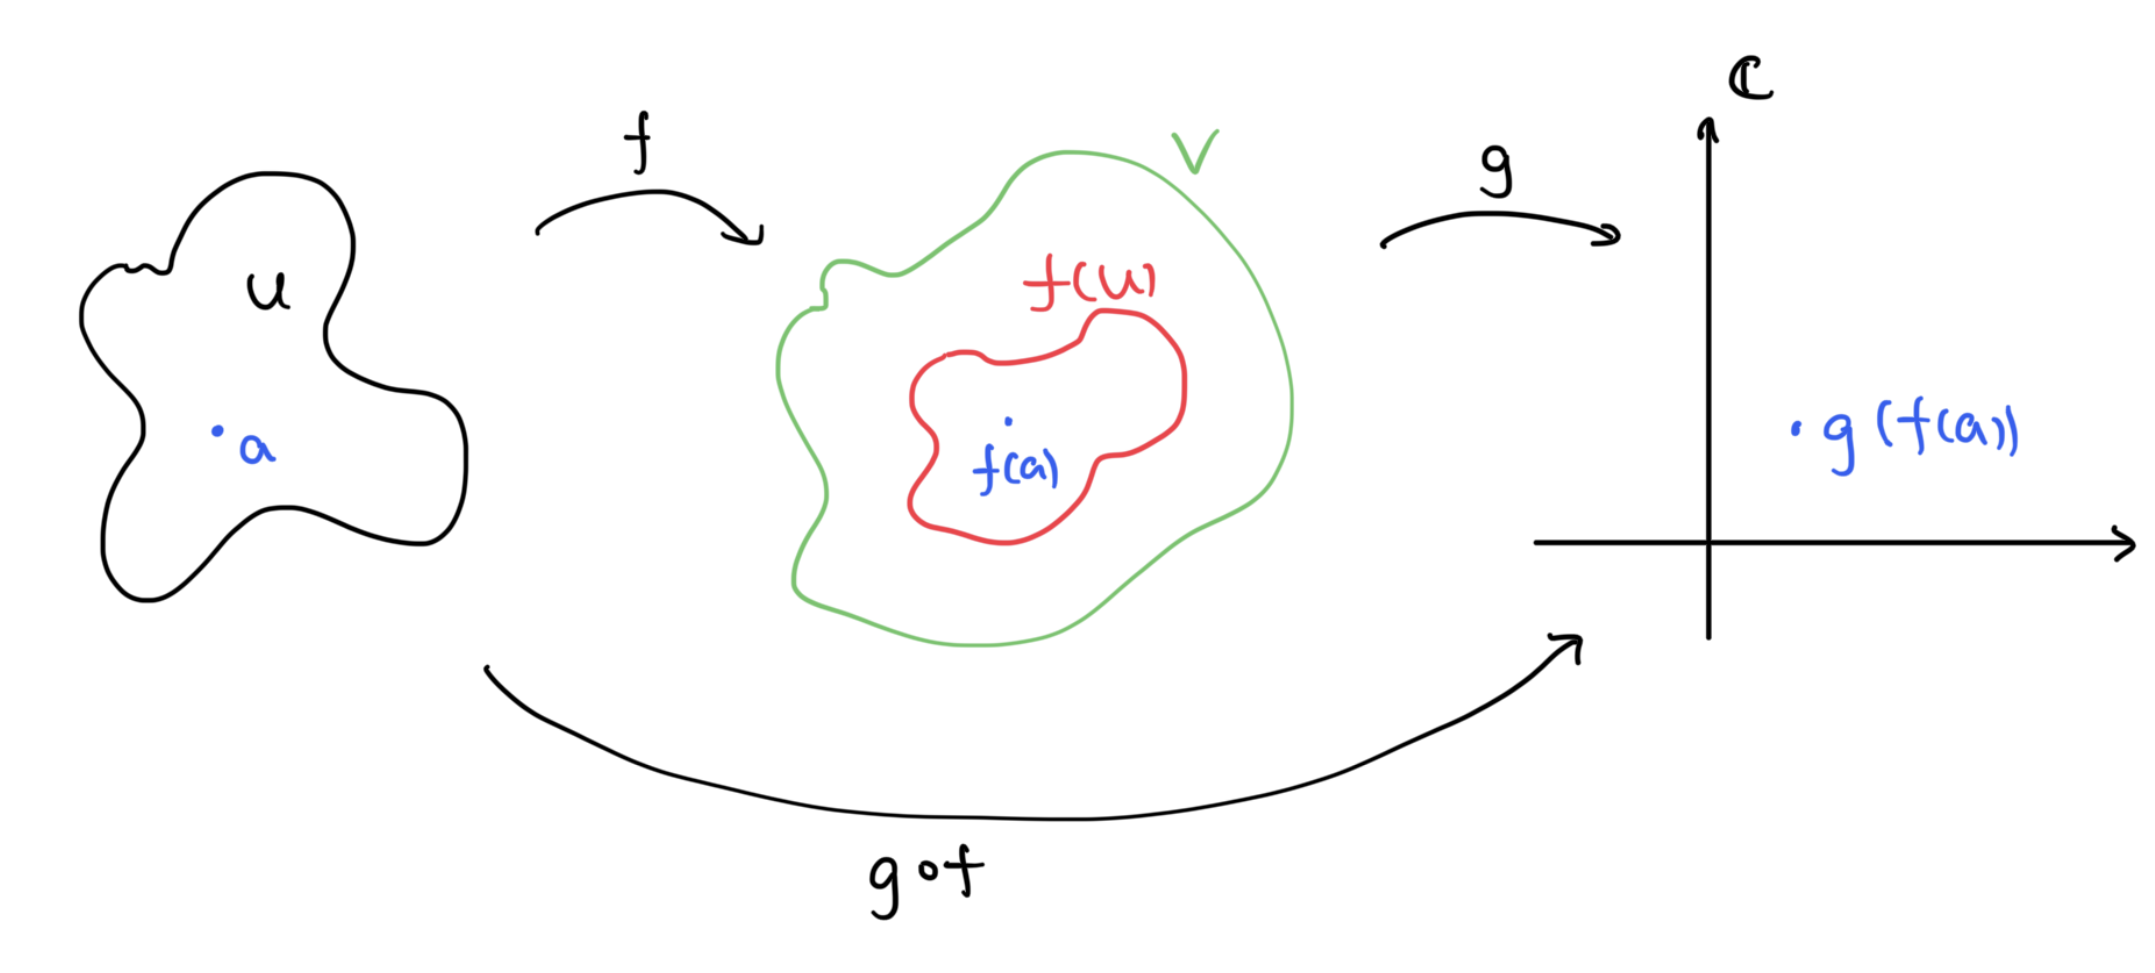
\includegraphics[scale=0.4]{fig/function-composition-continuity.png}
    \caption{Function Composition preserves Continuity}
    \label{fig:fn-composition-continuous}%
\end{figure}

\autoref{fig:fn-composition-continuous} visualises the condition required in \autoref{lem:fn-composition-continuous}.

\begin{proof}
    Since \(g\) is continuous at \(f\pqty{a}\), for \(\epsilon > 0\), we have some \(\sigma = \sigma\pqty{\epsilon} > 0\), such that
    \[
        y \in V, \abs{y - f\pqty{a}} < \sigma \implies \abs{g\pqty{y} - g\pqty{f\pqty{a}}} < \epsilon.
    \]

    On the other hand, since \(f\) is continuous at \(a\), there is some \(\delta = \delta\pqty{\sigma}\) for \(\sigma > 0\), that
    \[
        z \in U, \abs{z - a} < \delta \implies \abs{f\pqty{z} - f\pqty{a}} < \sigma.
    \]

    Therefore,
    \begin{align*}
        \forall \epsilon > 0, \exists \delta = \delta{\epsilon}: & z \in U, \abs{z - a} < \delta \\
        & \implies f\pqty{z} \in V, \abs{f\pqty{z} - f\pqty{a}} < \sigma \\
        & \implies \abs{g\pqty{f\pqty{z}} - g\pqty{f\pqty{a}}} < \epsilon
    \end{align*}
    as desired.
\end{proof}

\subsection{Extreme Value Theorem}

We first discuss some topology on \(\CC\).

\begin{definition}[Closed Set on \(\CC\)]
    \label{def:closed-set-c}%
    A set \(X \subseteq \CC\) is \term{closed} if it contains all its limit/accumulation points. Equivalently, all sequences \(\pqty{x_n}\) in \(X\) which converge in \(\CC\) have \(\lim_{n \in \infty} x_n \in X\).
\end{definition}

\begin{examples}[Closed Set on \(\RR\)]
    \label{ex:closed-set-r}%
    The closed interval \(\ccintv{0}{1}\) is closed. The open interval \(\oointv{0}{1}\) is not closed, and neither are \(\cointv{0}{1}\) and \(\ocintv{0}{1}\). However, the interval \(\cointv{0}{\plusinfty}\) is closed, while \(\oointv{0}{\plusinfty}\) is not.
\end{examples}

\begin{definition}[Bounded Set on \(\CC\)]
    \label{def:bounded-set-c}%
    Say \(X \subseteq \CC\) is \term{bounded}, if there is some \(M > 0\) such that
    \[
        X \subseteq \set{z \in \CC}{\abs{z} \leq M}.
    \]

    In other words, \(X\) is bounded if and only if \(\sup_{z \in X} \abs{z} < \infty\).
\end{definition}

\begin{examples}[Bounded Set on \(\RR\)]
    \label{ex:bounded-set-r}%
    The intervals \(\ccintv{0}{1}, \oointv{0}{1}, \cointv{0}{1}, \ocintv{0}{1}\) are bounded, while \(\cointv{0}{\plusinfty}\) and \(\oointv{0}{\plusinfty}\) are not bounded.
\end{examples}

\begin{definition}[Compact Set]
    \label{def:compact-set}%
    A set \(X \subseteq \CC\) is \term{compact} if it is closed and bounded.
\end{definition}

\begin{remark}
    If we are working in \(\RR\), we may think of compact sets as finite, closed intervals, i.e., \(\ccintv{a}{b}\) for \(a \leq b\).
\end{remark}

The main result of this section is technically \autoref{thm:continuity-compactness}, since it applies to more general spaces, rather than \autoref{thm:extreme-value}, which only applies to \(\RR\).

\begin{theorem}[Continuity Preserves Compactness]
    \label{thm:continuity-compactness}%
    Let \(X \subseteq \CC\) be compact. If \(\functiondomain{f}{X}{\CC}\) is continuous, then \(f\pqty{X} \subseteq \CC\) is compact.
\end{theorem}

A corollary of \autoref{thm:continuity-compactness} on \(\RR\) is \autoref{thm:extreme-value} (Extreme Value Theorem).

\begin{theorem}[Extreme Value Theorem]
    \label{thm:extreme-value}%
    Let \(X \subseteq \RR\) be compact. If \(\functiondomain{f}{X}{\RR}\) is continuous, then there is some \(a, b \in X\), such that
    \[
        f\pqty{a} = \sup f\pqty{X} = \sup_{z \in X} f\pqty{z}
    \]
    and
    \[
        f\pqty{b} = \inf f\pqty{X} = \inf_{z \in X} f\pqty{z}.
    \]
\end{theorem}

\begin{remark}
    The least upper bound axiom only tells us that the supremum and infimum exist for \(f\pqty{X}\). The point of \autoref{thm:extreme-value} (Extreme Value Theorem) is stating that these are in fact \emph{maximum} and \emph{minimum}.
\end{remark}

\begin{proof}[\proofname\ of \autoref{thm:extreme-value} (Extreme Value Theorem)]
    We focus on the first equality regarding the supremum, since the second proof is analogous.

    First, by \autoref{thm:continuity-compactness} (Continuity Preserves Compactness), since \(X\) is compact, \(f\pqty{X}\) is compact, hence bounded, and therefore let
    \[
        M = \sup f\pqty{X} \in \RR.
    \]

    By definition, \(\pqty{M - \frac{1}{n}}\) is not an upper bound of \(f\pqty{X}\) for any \(n \in \NN\). Hence, we can find a sequence \(\pqty{y_n}\) on \(f\pqty{X}\), such that
    \[
        M - \frac{1}{n} < y_n \leq M.
    \]

    Note that there is \(x_n \in X\) such that \(y_n = f\pqty{x_n}\). So we have a sequence \(\pqty{f\pqty{x_n}}\) on \(f\pqty{X}\), with
    \[
        M - \frac{1}{n} < f\pqty{x_n} \leq M.
    \]

    Now, taking limits, we have
    \[
        M \leq \lim_{n \to \infty} f\pqty{x_n} \leq M,
    \]
    and hence using the fact that \(f\) is continuous, using \autoref{thm:bolzano-weierstrass} (Bolzano--Weierstrass Theorem) to give a subsequence of the bounded sequence \(\pqty{x_n}\), say \(\pqty{x_{n_k}} \to x\),
    \[
        M = \lim_{n \to \infty} y_n = \lim_{k \to \infty} y_{n_k} = \lim_{k \to \infty} f\pqty{x_{n_k}} = f\pqty{\lim_{k \to \infty} x_{n_k}} = f\pqty{x}.
    \]

    Since \(f\pqty{X}\) is compact, it is closed, so \(x \in X\), and hence
    \[
        M = f\pqty{x} \in f\pqty{X},
    \]
    which finishes our proof.
\end{proof}

Now we prove \autoref{thm:continuity-compactness} (Continuity Preserves Compactness).

\begin{proof}[\proofname\ of \autoref{thm:continuity-compactness}, that \(f\pqty{X}\) is Bounded]
    Suppose on the contrary that \(f\pqty{X}\) is not bounded. Then for each \(n \in \NN\), we can find \(x_n \in X\), such that \(\abs{f\pqty{x_n}} > n\). Now, note \(\pqty{x_n}\) is a sequence in \(X\), and hence it is bounded since \(X\) is bounded.
    
    Applying \autoref{thm:bolzano-weierstrass} (Bolzano--Weierstrass Theorem), we have a convergent subsequence \(\pqty{x_{n_k}}_{k \in \NN}\) and \(x \in \CC\) such that \(x_{n_k} \to x\). But since \(X\) is closed, in fact we have \(x \in X\).
    
    On the other hand, we have
    \[
        \abs{f\pqty{x_{n_k}}} > n_k \geq k
    \]
    so the sequence \(f\pqty{x_{n_k}}\) cannot converge as \(k \to \infty\), since it is not bounded. This means \(f\) cannot be continuous, giving a contradiction.
\end{proof}

\begin{proof}[\proofname\ of \autoref{thm:continuity-compactness}, that \(f\pqty{X}\) is Closed]
    Take a sequence \(\pqty{y_n}\) in \(f\pqty{X}\) and suppose it converges to some \(y \in \CC\). We want to show that \(y \in f\pqty{X}\).

    Since \(y_n \in f\pqty{X}\), we have some \(x_n \in X\), such that \(f\pqty{x_n} = y_n\). The sequence \(\pqty{x_n}\) is on \(X\), and hence is bounded.
    
    By \autoref{thm:bolzano-weierstrass} (Bolzano--Weierstrass Theorem), we have a convergent subsequence \(\pqty{x_{n_k}}_{k \in \NN}\) that converges to some \(x\), and we have \(x \in X\) since \(X\) is closed.

    Therefore, by continuity, we have
    \[
        y = \lim_{n \to \infty} y_n = \lim_{k \to \infty} y_{n_k} = \lim_{k \to \infty} f\pqty{x_{n_k}} = f\pqty{\lim_{k \to \infty} x_{n_k}} = f\pqty{x},
    \]
    so \(y = f\pqty{x} \in f\pqty{X}\).
\end{proof}

\subsection{Intermediate Value Theorem}

\begin{theorem}[Intermediate Value Theorem]
    \label{thm:intermediate-value}%
    Let \(\functiondomain{f}{\ccintv{a}{b}}{\RR}\) be continuous. Then for any \(y\) between \(f\pqty{a}\) and \(f\pqty{b}\), there is some \(c \in \ccintv{a}{b}\), such that \(f\pqty{c} = y\).
\end{theorem}

\begin{figure}[ht!]
    \centering
    \begin{tikzpicture}[
        declare function = { f(\x) = (\x - 3) * (\x - 4) * (\x - 5) + 7; }
    ]
        \begin{axis}[
            axis lines = middle,
            xlabel = {\(x\)},
            ylabel = {\(f\pqty{x}\)},
            xmin = 0, xmax = 8,
            ymin = 0, ymax = 14,
            samples = 100,
            domain = 2:6,
            xtick = {\xa, \xc, \xb},
            xticklabels = {\(a\), \(c\), \(b\)},
            ytick = {\yc},
            yticklabels = {\(y\)}
        ]
            \pgfmathsetmacro{\xa}{2.5}
            \pgfmathsetmacro{\ya}{f(\xa)}
            \pgfmathsetmacro{\xb}{5.2}
            \pgfmathsetmacro{\yb}{f(\xb)}
            \pgfmathsetmacro{\xc}{4}
            \pgfmathsetmacro{\yc}{f(\xc)}

            \addplot[no marks] {f(x)};
            \node[right] at (axis cs:6, 13) {\(f\)};

            \addplot[only marks, mark=*, mark size=1pt]
                coordinates {(\xa, \ya) (\xb, \yb) (\xc, \yc)};

            \node[above left] at (axis cs:\xa, \ya) {\(\pqty{a, f\pqty{a}}\)};
            \node[below right] at (axis cs:\xb, \yb) {\(\pqty{b, f\pqty{b}}\)};
            \node[below left] at (axis cs:\xc, \yc) {\(\pqty{c, y}\)};

            \addplot[dotted] coordinates {(0, \yc) (\xc, \yc) (\xc, 0)};
        \end{axis}
    \end{tikzpicture}

    \caption{Intermediate Value Theorem}
    \label{fig:intermediate-value}
\end{figure}

\begin{corollary}[Continuous Functions maps Closed Intervals to Closed Intervals]
    \label{cor:continuous-closed-intv}%
    If \(\functiondomain{f}{\ccintv{a}{b}}{\RR}\) is continuous, then its image \(\img f = f\pqty{\ccintv{a}{b}}\) is a closed interval.
\end{corollary}

\begin{proof}
    From \autoref{thm:extreme-value} (Extreme Value Theorem) we know that \(\min_{x \in \ccintv{a}{b}} f\pqty{x}\) and \(\max_{x \in \ccintv{a}{b}} f\pqty{x}\) exist. Let \(f\pqty{c} = \min_{x \in \ccintv{a}{b}} f\pqty{x}\) and \(f\pqty{d} = \max_{x \in \ccintv{a}{b}} f\pqty{x}\) for some \(c, d \in \ccintv{a}{b}\).

    Applying \autoref{thm:intermediate-value} (Intermediate Value Theorem) shows that we indeed get all values between the minimum and the maximum, showing the image is indeed the closed interval
    \[
        \ccintv{\min_{x \in \ccintv{a}{b}} f\pqty{x}}{\max_{x \in \ccintv{a}{b}} f\pqty{x}}.
    \]
\end{proof}

\begin{remark}
    \autoref{thm:intermediate-value} (Intermediate Value Theorem) guarantees \emph{existence} but not \emph{uniqueness}. In particular, there may be several points whose image is \(y\) above.
\end{remark}

\begin{proof}[\proofname\ of \autoref{thm:intermediate-value} (Intermediate Value Theorem)]
    If \(f \pqty{a} = f\pqty{b}\), then this is trivially true. Furthermore, if \(y = f\pqty{a}\) or \(y = f\pqty{b}\) then this is trivially true.

    Now, we let \(f\pqty{a} < y < f\pqty{b}\). Set
    \[
        S = \set{x \in \ccintv{a}{b}}{f\pqty{x} \leq y}.
    \]

    Then \(a \in S\), so \(S\) is non-empty, and \(S\) is bounded above, so let
    \[
        c = \sup S \in \ccintv{a}{b}.
    \]

    We claim that \(f\pqty{c} = y\).

    We first show that \(f\pqty{c} \leq y\). Suppose not, then \(f\pqty{c} > y\), so in particular, \(c > a\). Let \(\epsilon = f\pqty{c} - y > 0\). By the continuity of \(f\), we have some \(\delta > 0\), such that
    \[
        \abs{x - c} < \delta, x \in \ccintv{a}{b} \implies \abs{f\pqty{x} - f\pqty{c}} < \epsilon.
    \]

    Therefore, we have
    \[
         \abs{x - c} < \delta, x \in \ccintv{a}{b} \implies \abs{f\pqty{x} - f\pqty{c}} < \epsilon \implies f\pqty{x} > f\pqty{c} - \epsilon = y \implies x \notin S.
    \]

    Let \(I = \oointv{c - \delta}{c} \cap \ccintv{a}{b}\). \(I\) is non-empty since \(c > a\).

    Consider \(I \cap S\). This intersection is non-empty since \(c > a\) and \(a \in S\), by the definition of a supremum. However, from above, \(x \in I \implies x \notin S\), so \(I \cap S\) is empty. This gives a contradiction.

    Next, we show \(f\pqty{c} \geq y\). Suppose not, then \(f\pqty{c} < y\), so in particular, \(c < b\). Let \(\epsilon = y - f\pqty{c} > 0\). By continuity of \(f\), we have \(\delta > 0\) such that
    \[
        \abs{x - c} < \delta, x \in \ccintv{a}{b} \implies \abs{f\pqty{x} - f\pqty{c}} < \epsilon.
    \]

    Therefore, we have
    \[
        \abs{x - c} < \delta, x \in \ccintv{a}{b} \implies \abs{f\pqty{x} - f\pqty{c}} < \epsilon \implies f\pqty{x} < f\pqty{c} + \epsilon = y \implies x \in S.
    \]
    
    Let \(I = \oointv{c}{c + \delta} \cap \ccintv{a}{b}\). This intersection is non-empty since \(c < b\).
    
    Consider \(I \cap S\). This intersection is empty by the definition of a supremum. However, from above, \(x \in I \implies x \in S\), so \(I \cap S\) is non-empty. This gives a contradiction.

    Therefore, \(f\pqty{c} = y\), finishing the proof.
\end{proof}

\begin{example}[Existence of \(N\)-th Roots]
    \label{ex:existence-nth-roots}%
    We can apply to show the existence of \(N\)-th roots. Take \(t > 0\), and consider
    \[
        \function{f}{\ccintv{0}{1 + t}}{\RR}{x}{x^N}
    \]
    for some \(N \in \NN\). This is a continuous function, and we have
    \[
        0 = f\pqty{0} < t < \pqty{1 + t}^N = f\pqty{1 + t}.
    \]

    By \autoref{thm:intermediate-value}, there is some \(c \in \ccintv{0}{1 + t}\) such that \(f\pqty{c} = t\), and for this value of \(c\), we have \(c^N = t\). Hence, \(c\) is \emph{an} \(N\)-th positive root of \(t\).
\end{example}

\begin{definition}[Monotone Function]
    \label{def:monotone-function}%
    A function \(\functiondomain{f}{\ccintv{a}{b}}{\RR}\) is \term{monotone}, if it is either
    \begin{itemize}
        \item \term{increasing}, if for all \(a \leq x_1 \leq x_2 \leq b\), we have \(f\pqty{x_1} \leq f\pqty{x_2}\); or
        \item \term{decreasing}, if for all \(a \leq x_1 \leq x_2 \leq b\), we have \(f\pqty{x_1} \geq f\pqty{x_2}\).
    \end{itemize}

    We say the function is \term{strictly increasing/decreasing} for the condition modified to \(f\pqty{x_1} < f\pqty{x_2}\) or \(f\pqty{x_1} > f\pqty{x_2}\).
\end{definition}

\begin{theorem}[Inverse Function Theorem for Monotone Functions]
    \label{thm:inverse-fn-thm-monotone}
    Let \(\functiondomain{f}{\ccintv{a}{b}}{\RR}\) be continuous and strictly monotone. We set \(c = \min\set{f\pqty{a}, f\pqty{b}}\) and \(d = \max\set{f\pqty{a}, f\pqty{b}}\). Then the restriction of the co-domain
    \[
        \functiondomain{f}{\ccintv{a}{b}}{\ccintv{c}{d}}
    \]
    is bijective, and \(\functiondomain{f\inverse}{\ccintv{c}{d}}{\ccintv{a}{b}}\) exists, is continuous and strictly monotone, with the same monotonicity as \(f\).
\end{theorem}

\begin{proof}
    Strict monotonicity tells us that the maximum and minimum must be obtained at endpoints, therefore the restriction of the co-domain is well-defined. We start by showing that \(f\), when its co-domain is restricted, is bijective. \autoref{cor:continuous-closed-intv} shows that \(f\) is surjective, and strict monotonicity guarantees injectivity.

    Without loss of generality, let \(f\) be strictly increasing. Let \(\functiondomain{f\inverse}{\ccintv{c}{d}}{\ccintv{a}{b}}\). Suppose, on the contrary, that \(f\inverse\) is not strictly increasing. Then there is some \(c \leq y_1 < y_2 \leq d\) with \(f\inverse\pqty{y_1} \geq f\inverse\pqty{y_2}\). This means \(a \leq f\inverse\pqty{y_2} \leq f\inverse\pqty{y_1} \leq b\). Applying \(f\), and using that \(f\) is strictly increasing, we see
    \[
        f \circ f\inverse\pqty{y_2} \leq f \circ f\inverse\pqty{y_1}
    \]
    so
    \[
        y_2 \leq y_1
    \]
    giving a contradiction with \(y_1 < y_2\). This shows that \(f\inverse\) is indeed strictly increasing.

    We need to check continuity of \(f\inverse\). Fix \(y_0 \in \ccintv{c}{d}\) and let \(x_0 = f\inverse\pqty{y_0}\). We consider the three cases for \(x_0\) and \(y_0\), in particular when they are endpoints of the interval.

    \begin{itemize}
        \item \(x_0 \in \oointv{a}{b}\). Let \(\epsilon > 0\) be arbitrary. Let \(\eta \in \ocintv{0}{\epsilon}\) be sufficiently small that \(\ccintv{x_0 - \eta}{x_0 + \eta} \in \ccintv{a}{b}\). Since \(f\) is strictly increasing, we have
        \[
            f\pqty{x_0 - \eta} < f\pqty{x_0} = y_0 < f\pqty{x_0 + \eta}.
        \]

        We take \(\delta = \min\set{f\pqty{x_0 + \eta} - y_0, y_0 - f\pqty{x_0 - \eta}} > 0\). We have
        \begin{align*}
            \abs{y - y_0} < \delta, y \in \ccintv{c}{d} &\implies f\pqty{x_0 - \eta} \leq y_0 - \delta < y < y_0 + \delta \leq f\pqty{x_0 + \eta} \\
            &\implies f\pqty{x_0 - \eta} < y < f\pqty{x_0 + \eta} \\
            &\implies x_0 - \eta < f\inverse\pqty{y} = x_0 < x+0 + \eta \\
            &\implies \abs{f\inverse\pqty{y} - x_0} < \eta \\
            &\implies \abs{f\inverse\pqty{y} - f\inverse\pqty{y_0}} < \epsilon
        \end{align*}
        as desired.

        \item \(x_0 = a\), and we have \(y_0 = f\pqty{a}\). Fix \(\epsilon > 0\), and we choose \(\eta = \min\set{\epsilon, b - a}\), and set \(\delta = f\pqty{a + \eta} - f\pqty{a} > 0\). We have
        \begin{align*}
            \abs{y - y_0} < \delta, y \in \ccintv{c}{d} &\implies f\pqty{a} \leq y \leq f\pqty{a + \eta} \\
            &\implies a \leq f\inverse\pqty{y} \leq a + \eta \\
            &\implies \abs{f\inverse\pqty{y} - f\inverse\pqty{y_0}} < \eta \leq \epsilon.
        \end{align*}

        \item The case where \(x_0 = b\) is similar.
    \end{itemize}

    So \(f\) is continuous at any point \(y_0 \in \ccintv{c}{d}\), which implies that \(f\inverse\) is continuous.
\end{proof}
\section{Differentiation}
\subsection{Basics}

Informally, the derivative of a function is the instantaneous rate of change of a function at that point. \autoref{fig:derivative} shows a way to think about the gradient at some point \(c \in \ccintv{a}{b}\) -- namely approximating the gradient of a secant \(\frac{\delta y}{\delta x}\), and taking the limit as \(h = \delta x \to 0\).

\begin{figure}[ht!]
    \centering
    \begin{tikzpicture}[
        declare function = { f(\x) = 0.6 * (\x - 3) * (\x - 4) * (\x - 5) + 1.5 * (\x - 4) + 7; }
    ]
        \begin{axis}[
            axis lines = middle,
            xlabel = {\(x\)},
            ylabel = {\(f\pqty{x}\)},
            xmin = 0, xmax = 8,
            ymin = 0, ymax = 14,
            samples = 100,
            domain = 2:6,
            xtick = {\xa, \xb, \xc, \xd},
            xticklabels = {\(a\), \(b\), \(c\), \(c + h\)},
            ytick = {\ya, \yb, \yc, \yd},
            yticklabels = {\(f\pqty{a}\), \(f\pqty{b}\), \(f\pqty{c}\), \(f\pqty{c + h}\)}
        ]

            \pgfmathsetmacro{\xa}{2}
            \pgfmathsetmacro{\ya}{f(\xa)}
            \pgfmathsetmacro{\xb}{6}
            \pgfmathsetmacro{\yb}{f(\xb)}
            \pgfmathsetmacro{\xc}{3.5}
            \pgfmathsetmacro{\yc}{f(\xc)}
            \pgfmathsetmacro{\xd}{4.5}
            \pgfmathsetmacro{\yd}{f(\xd)}

            \addplot[no marks] {f(x)};
            \node[right] at (axis cs: 6, 13) {\(f\)};

            \addplot[only marks, mark=*, mark size=1pt]
                coordinates {(\xa, \ya) (\xb, \yb) (\xc, \yc) (\xd, \yd)};

            \addplot[dotted] coordinates {(0, \ya) (\xa, \ya) (\xa, 0)};
            \addplot[dotted] coordinates {(0, \yb) (\xb, \yb) (\xb, 0)};
            \addplot[dotted] coordinates {(0, \yc) (\xc, \yc) (\xc, 0)};
            \addplot[dotted] coordinates {(0, \yd) (\xd, \yd) (\xd, 0)};

            \draw[<->] (axis cs: \xc, \yc) -- (axis cs: \xd, \yc);

            \node[below] at (axis cs: {(\xc + \xd) / 2}, \yc) {\(\delta x\)};

            \draw[<->] (axis cs: \xc, \yc) -- (axis cs: \xc, \yd);

            \node[left] at (axis cs: \xc, {(\yc + \yd) / 2}) {\(\delta y\)};
        \end{axis}
    \end{tikzpicture}

    \caption{Derivative}
    \label{fig:derivative}
\end{figure}

\begin{definition}[Derivative]
    \label{def:derivative}%
    Let \(\functiondomain{f}{X \subseteq \CC}{\CC}\) and \(a \in X\) be an accumulation point. We say \(f\) is \term{differentiable} at \(a\), if we have
    \[
        \lim_{x \to a} \frac{f\pqty{x} - f\pqty{a}}{x - a} = \lim_{h \to 0} \frac{f\pqty{a + h} - f\pqty{a}}{h}
    \]
    exists. The value of this limit is the \term{derivative} of \(f\) evaluated at \(a\), denoted as \(f'\pqty{a}\) or \(\dv{f}{x} \pqty{a}\).
\end{definition}

\begin{remark}
    We cannot really make sense of the derivative at an isolated point of the domain, since the point is not in the domain of the fraction, and not an accumulation point of the domain of the fraction either -- so the limit is undefined.

    As for accumulation points, we can distinguish between \emph{interior points}, where we can approach that point along any direction (and we need the limit to be direction independent); and \emph{non-interior points} whose limit is restricted by the domain.
\end{remark}

\begin{examples}[Differentiability of Functions]
    \label{ex:differentiability}%
    \begin{itemize}
        \item We take the identity function \(f\pqty{z} = z\). We have
        \[
            f'\pqty{z} = \lim_{h \to 0} \frac{f\pqty{z + h} - f\pqty{z}}{h} = \lim_{h \to 0} \frac{\pqty{z + h} - z}{h} = \lim_{h \to 0} 1 = 1.
        \]

        \item We take the complex conjugate function \(f\pqty{z} = \conjugate{z}\). We claim this is not differentiable at \emph{any} point.
        
        We consider the limits \(h \to 0\) along the real axis and the complex axis separately.

        Take \(h = \lambda\) for \(\lambda \in \RR\), we have
        \[
            \lim_{\lambda \to 0} \frac{f\pqty{z + \lambda} - f\pqty{z}}{\lambda} = \lim_{\lambda \to 0} \frac{\bar{\lambda}}{\lambda} = \lim_{\lambda \to 0} \frac{\lambda}{\lambda} = 1
        \]
        and \(h = i \lambda\) for \(\lambda \in \RR\), we have
        \[
            \lim_{\lambda \to 0} \frac{f\pqty{z + i \lambda} - f\pqty{z}}{i\lambda} = \lim_{\lambda \to 0} \frac{\conjugate{i \lambda}}{i \lambda} = \lim_{\lambda \to 0} \frac{- i \lambda}{i \lambda} = -1.
        \]

        \item We consider the real sine function \(f\pqty{x} = \sin x\). We have
        \begin{align*}
            f'\pqty{x} &= \lim_{h \to 0} \frac{\sin \pqty{x + h} - \sin \pqty{x}}{h} \\
            &= \lim_{h \to 0} \frac{\sin \pqty{h} \cos x}{h} + \lim_{h \to 0} \frac{\sin x \pqty{\cos h - 1}}{h} \\
            &= \cos x \cdot 1 + 0 \\
            &= \cos x.
        \end{align*}
    \end{itemize}
\end{examples}

Differentiability is a stronger property than continuity -- indeed we cannot differentiate functions that are not continuous.

\begin{proposition}[Differentiability implies Continuity]
    \label{prop:differentiability-implies-continuity}%
    Let \(\functiondomain{f}{X \subseteq \CC}{\CC}\) be differentiable at some \(a \in X\). Then it is continuous at \(a\).
\end{proposition}

\begin{proof}
    Note that
    \begin{align*}
        \bqty{\lim_{h \to 0} f\pqty{a + h}} - f\pqty{a} &= \lim_{h \to 0} \bqty{f\pqty{a + h} - f\pqty{a}} \\
        &= \lim_{h \to 0} \frac{f\pqty{a + h} - f\pqty{a}}{h} \cdot h \\
        &= \lim_{h \to 0} \frac{f\pqty{a + h} - f\pqty{a}}{h} \cdot \lim_{h \to 0} h \\
        &= f'\pqty{a} \cdot 0 \\
        &= 0
    \end{align*}
    gives continuity as desired.
\end{proof}

We may derive properties of derivative from the properties of limits as well.

\begin{lemma}[Properties of Derivatives]
    \label{lem:properties-derivatives}%
    Let \(\functiondomain{f, g}{X \subseteq \CC}{\CC}\) be differentiable at \(a \in X\). Then the sum \(f\pqty{x} + g\pqty{x}\), the product \(f\pqty{x} \cdot g\pqty{x}\), and the reciprocal \(\frac{1}{f\pqty{x}}\) (if defined, i.e. if \(f\pqty{a} \neq 0\)) are all differentiable at \(a\). Furthermore, we have
    \begin{align*}
        \pqty{f + g}' \pqty{a} &= f'\pqty{a} + g'\pqty{a}, \\
        \pqty{fg}' \pqty{a} &= f'\pqty{a} g\pqty{a} + f\pqty{a} g'\pqty{a}, \\
        \pqty{\frac{1}{f}}' \pqty{a} &= - \frac{f'\pqty{a}}{\bqty{f\pqty{a}}^2}.
    \end{align*}
\end{lemma}

\begin{proof}
    The addition rule is trivial from \autoref{lem:fn-limits-preserve-arithmetic}.

    We now look at the product.
    \begin{align*}
        \pqty{fg}'\pqty{a} &= \lim_{h \to 0} \frac{\pqty{fg}\pqty{a + h} - \pqty{fg}\pqty{a}}{h} \\
        &= \lim_{h \to 0} \frac{f\pqty{a + h} g\pqty{a + h} - f\pqty{a} g\pqty{a}}{h} \\
        &= \lim_{h \to 0} \frac{\pqty{f\pqty{a + h} - f\pqty{a}} g\pqty{a + h} + \pqty{g\pqty{a + h} - g\pqty{a}} f\pqty{a}}{h} \\
        &= \lim_{h \to 0} g\pqty{a + h} \cdot \lim_{h \to 0} \frac{f\pqty{a + h} - f\pqty{a}}{h} + f\pqty{a} \cdot \lim_{h \to 0} \frac{g\pqty{a + h} - g\pqty{a}}{h} \\
        &= g\pqty{a} \cdot f'\pqty{a} + f\pqty{a} \cdot g'\pqty{a},
    \end{align*}
    using continuity (implied by differentiability, stated in \autoref{prop:differentiability-implies-continuity}), in \(\lim_{h \to 0} g\pqty{a + h} = g\pqty{a}\).

    As for the reciprocal,
    \begin{align*}
        \pqty{\frac{1}{f}}'\pqty{a} &= \lim_{h \to 0} \frac{\frac{1}{f\pqty{a + h}} - \frac{1}{f\pqty{a}}}{h} \\
        &= \lim_{h \to 0} \frac{f\pqty{a} - f\pqty{a + h}}{h} \cdot \frac{1}{f\pqty{a} f\pqty{a + h}} \\
        &= - \lim_{h \to 0} \frac{1}{f\pqty{a} f\pqty{a + h}} \cdot \lim_{h \to 0} \frac{f\pqty{a + h} - f\pqty{a}}{h} \\
        &= - \frac{f'\pqty{a}}{\bqty{f\pqty{a}}^2}.
    \end{align*}
\end{proof}

\begin{examples}[Applications of Differentiation Rules]
    \label{ex:application-of-differentiation-rules}%
    \begin{itemize}
        \item Let \(f\pqty{z} = z^2\), then it is differentiable with \(f'\pqty{z} = 2z\). By induction, for \(f\pqty{z} = z^n\) with \(n \in \NN\), we have \(f'\pqty{z} = n z^{n - 1}\).
        \item Let \(f\pqty{z} = \frac{1}{z}\). It is differentiable on \(\CC \setminus\Bqty{0}\) with \(f'\pqty{z} = -\frac{1}{z^2}\). By induction, for \(f\pqty{z} = \frac{1}{z^n}\), we have \(f'\pqty{z} = - \frac{n}{z^{n + 1}}\).
        \item More generally, rational functions \(\frac{p\pqty{x}}{q\pqty{x}}\) for polynomials \(p, q\) are differentiable, wherever it is defined.
    \end{itemize}
\end{examples}

\begin{proposition}[Chain Rule]
    \label{prop:chain-rule}%
    Let \(U, V \subseteq \CC\), and let \(\functiondomain{f}{U}{V}\), and \(\functiondomain{g}{V}{\CC}\). Suppose \(f\) is differentiable at some \(a \in U\), and \(g\) is differentiable at some \(f\pqty{a} \in V\). Then the composition \(g \circ f\) is differentiable at \(a\), and that
    \[
        \pqty{g \circ f}'\pqty{a} = g' \pqty{f\pqty{a}} \cdot f'\pqty{a}.
    \]
\end{proposition}

\begin{proof}
    One might be very tempted to say that
    \[
        \frac{g\pqty{f\pqty{x}} - g\pqty{f\pqty{a}}}{x - a} = \frac{g\pqty{f\pqty{x}} - g\pqty{f\pqty{a}}}{f\pqty{x} - f\pqty{a}} \cdot \frac{f\pqty{x} - f\pqty{a}}{x - a}
    \]
    and this finishes the proof. However, we need to deal with the case where we are dividing by zero. Therefore, we define a helper function
    \[
        Q\pqty{y} = \begin{cases}
            \frac{g\pqty{y} - g\pqty{f\pqty{a}}}{y - f\pqty{a}}, & y \neq f\pqty{a}, \\
            g'\pqty{f\pqty{a}}, & y = f\pqty{a},
        \end{cases}
    \]
    and we claim that the quotient is always equal to
    \[
        Q\pqty{f\pqty{x}} \cdot \frac{f\pqty{x} - f\pqty{a}}{x - a}.
    \]

    For any \(x \neq a\), if \(f\pqty{x} \neq f\pqty{a}\), then the equality is from the cancellation of fraction from above. If \(x \neq a\) but \(f\pqty{x} = f\pqty{a}\), then the quotient is zero, and this expression is zero as well since the second term is zero.

    Now it remains to take the limit of this expression. As \(x \to a\), the second factor tends to \(f'\pqty{a}\). For \(Q\pqty{y}\), note that since \(g\) is differentiable at \(f\pqty{a}\), so we have
    \[
        \lim_{y \to f\pqty{a}} Q\pqty{y} = g'\pqty{f\pqty{a}} = Q\pqty{f\pqty{a}}
    \]
    so \(Q\) is continuous at \(f\pqty{a}\). Furthermore, \(f\) is differentiable at \(a\), and hence continuous. Therefore, \(Q \circ f\) is continuous at \(a\), so its limit is simply \(Q\circ f\pqty{a} = g'\pqty{f\pqty{a}}\).

    Taking the product of the limit of the two factors, we have
    \[
        g \circ f'\pqty{a} = g'\pqty{f\pqty{a}} \cdot f'\pqty{a}
    \]
    as desired.
\end{proof}

We may provide another characterisation of the derivative to give a proof of \autoref{prop:chain-rule} (Chain Rule) which could be generalised to higher dimensions.

We have seen that \(f'\pqty{a}\) is the slope of the tangent line to the graph of \(f\) at \(a\). We can formalise this in the following way.

\begin{lemma}[Linear Approximation and Differentiability]
    \label{lem:linear-approximation-differentiability}%
    Let \(\functiondomain{f}{X \subseteq \CC}{\CC}\). Then \(f\) be differentiable at \(a\), if and only if there is some \(A \in \CC\), and a function \(\functiondomain{\epsilon}{\set{z \in \CC}{z + a \in X}}{\CC}\) (an error function), with \(\epsilon\pqty{h} \to 0\) as \(h \to 0\), such that
    \[
        f\pqty{a + h} = f\pqty{a} + A h + \epsilon\pqty{h} \abs{h}.
    \]

    In particular, such \(A\) is \(f'\pqty{a}\).
\end{lemma}

\begin{remark}
    This says that \(f\pqty{a + h}\) is approximately \(f\pqty{x} + Ah\), and the error function \(\epsilon\pqty{h}\) is to quantify the error in this approximation. This is also much easier to generalise to higher dimensions for functions in more general spaces (Banach spaces). In this more general case, \(A\) will be a linear operator.
\end{remark}

We can also write that \(f\pqty{a + h} = f\pqty{a} + Ah + \littleO\pqty{h}\) using the little-\(\littleO\) notation (and not big-\(\bigO\)) to mean the same thing.

\begin{proof}[\proofname\ of \autoref{lem:linear-approximation-differentiability}]
    We assume there is such linear approximation. Then
    \begin{align*}
        \lim_{h \to 0} \frac{f\pqty{a + h} - f\pqty{a}}{h} &= \lim_{h \to 0} \frac{Ah + \epsilon\pqty{h} \cdot \abs{h}}{h} \\
        &= A + \lim_{h \to 0} \pqty{\epsilon\pqty{h} \cdot \frac{\abs{h}}{h}} \\
        &= A + 0 \\
        &= A,
    \end{align*}
    since \(\frac{\abs{h}}{h}\) is bounded and \(\epsilon\pqty{h} \to 0\). Therefore, \(f\) is differentiable at \(a\), and hence \(f'\pqty{a} = A\).

    On the other hand, if the function is differentiable at \(a\), let \(A = f'\pqty{a}\). We take the error function
    \[
        \epsilon\pqty{h} = \begin{cases}
            \frac{f\pqty{a + h} - f\pqty{a} - Ah}{\abs{h}}, & h \neq 0, \\
            0, & h = 0.
        \end{cases}
    \]
    Then we can see by taking limits that \(\epsilon\pqty{h} \to 0\) as \(h \to 0\).
\end{proof}

\begin{proof}[\proofname\ of \autoref{prop:chain-rule} (Chain Rule)]
    Since \(f, g\) are differentiable at \(a, f\pqty{a}\) respectively, there exist some error functions \(\epsilon_f, \epsilon_g\) such that \(\epsilon_f\pqty{h}, \epsilon_g\pqty{h} \to 0\) as \(h \to 0\), and that
    \[
        f\pqty{a + h} = f\pqty{a} + f'\pqty{a} h + \epsilon_f\pqty{h} \abs{h}
    \]
    and similarly
    \[
        g\pqty{f\pqty{a} + k} = g\pqty{f\pqty{a}} + g'\pqty{f\pqty{a}} k + \epsilon_g\pqty{k} \abs{k}.
    \]

    We now investigate the composition. Note that
    \begin{align*}
        g \circ f\pqty{a + h} - g \circ f\pqty{a} &= g\pqty{f\pqty{a + h}} - g\pqty{f\pqty{a}} \\
        &= g\pqty{f\pqty{a} + f'\pqty{a} h + \epsilon_f\pqty{h} \abs{h}} - g\pqty{f\pqty{a}} \\
        &= g\pqty{f\pqty{a}} + g'\pqty{f\pqty{a}} \cdot k + \epsilon_g \pqty{k} \cdot \abs{k} - g\pqty{f\pqty{a}} \\
        &= g'\pqty{f\pqty{a}} \cdot k + \epsilon_g\pqty{k} \abs{k}
    \end{align*}
    where we let
    \[
        k = f'\pqty{a}h + \epsilon_f\pqty{h} \abs{h}.
    \]

    Hence,
    \begin{align*}
        g \circ f\pqty{a + h} - g \circ f\pqty{a} &= g'\pqty{f\pqty{a}} f'\pqty{a} h + g'\pqty{f\pqty{a}} \epsilon_f\pqty{h} \abs{h} + \epsilon_g\pqty{k} \abs{k} \\
        &= g'\pqty{f\pqty{a}} f'\pqty{a} h + \epsilon\pqty{h} \abs{h}
    \end{align*}
    where we let
    \[
        \epsilon\pqty{h} = g'\pqty{f\pqty{a}} \epsilon_f\pqty{h} + \epsilon_g\pqty{h f'\pqty{a} + \epsilon_f\pqty{h} \abs{h}} \cdot \abs{\pm f'\pqty{a} + \epsilon_f\pqty{h}},
    \]
    where the \(\pm\) sign arises since we extracted \(h\) with \(\abs{h}\) out from the absolute value of \(k\).

    We want to check that \(\epsilon\pqty{h} \to 0\) as \(h \to 0\). We conduct the limit term-by-term. Note that indeed,
    \[
        \lim_{h \to 0} \bqty{g'\pqty{f\pqty{a}} \epsilon_f\pqty{h}} = g'\pqty{f\pqty{a}} \lim_{h \to 0} \epsilon_f\pqty{h} = 0,
    \]
    and since the inside term of the function \(\epsilon_g\) satisfies
    \[
        \lim_{h \to 0} \bqty{h f'\pqty{a} + \epsilon_f\pqty{h} \abs{h}} = 0
    \]
    and also
    \[
        \lim_{h \to 0} \abs{\pm f'\pqty{a} + \epsilon_f\pqty{h}} = \abs{f'\pqty{a}},
    \]
    we have \(\epsilon\pqty{h} \to 0\). This proves the chain rule indeed.
\end{proof}

\begin{example}[Application of the Chain Rule]
    \label{ex:application-chain-rule}%
    We let
    \[
        f\pqty{x} = \begin{cases}
            x \sin \pqty{\frac{1}{x}}, & x \neq 0, \\
            0, & x = 0.
        \end{cases}
    \]

    At \(x \neq 0\), the chain rule gives us that
    \[
        f'\pqty{x} = 1 \cdot \sin \pqty{\frac{1}{x}} + x \cdot \cos \pqty{\frac{1}{x}} \cdot \pqty{- \frac{1}{x^2}} = \sin \pqty{\frac{1}{x}} - \frac{1}{x} \cos \pqty{\frac{1}{x}}.
    \]

    At \(x = 0\), we have
    \[
        f'\pqty{0} = \lim_{h \to 0} \frac{f\pqty{h} - f\pqty{0}}{h} = \lim_{h \to 0} \sin \pqty{\frac{1}{h}}
    \]
    does not exist. Hence, \(f\) is not differentiable at \(0\). \(f\) is differentiable on \(\RR \setminus \Bqty{0}\).
\end{example}

\autoref{lem:linear-approximation-differentiability} gives another way to prove \autoref{prop:differentiability-implies-continuity} (Differentiability implies Continuity).

\begin{proof}[\proofname\ of \autoref{prop:differentiability-implies-continuity}]
    Recall that we have
    \begin{align*}
        f\pqty{x} &= \lim_{h \to 0} f\pqty{a + h} \\
        &= \lim_{h \to 0} \pqty{f\pqty{a} + Ah + \epsilon\pqty{h} \cdot \abs{h}} \\
        &= f\pqty{a} + A \cdot \lim_{h \to 0} h + \lim_{h \to 0} \pqty{\epsilon\pqty{h} \cdot \abs{h}} \\
        &= f\pqty{a}.
    \end{align*}
\end{proof}

\subsection{Mean Value Theorems}

\begin{theorem}[Mean Value Theorem]
    \label{thm:mean-value-thm}%
    Let \(\functiondomain{f}{\ccintv{a}{b}}{\RR}\) be continuous on \(\ccintv{a}{b}\) and differentiable on \(\oointv{a}{b}\). Then there is some \(c \in \oointv{a}{b}\) such that
    \[
        f'\pqty{c} = \frac{f\pqty{b} - f\pqty{a}}{b - a}.
    \]
\end{theorem}

\begin{figure}[ht!]
    \centering
    \begin{tikzpicture}[
        declare function = { f(\x) = 0.3 * (\x - 1) * (\x - 3) * (\x - 5) + 3 + (\x - 3); }
    ]
        \begin{axis}[
            axis lines = middle,
            xlabel = {\(x\)},
            ylabel = {\(y\)},
            xmin = -0.5, xmax = 6.5,
            ymin = -0.5, ymax = 6.5,
            samples = 200,
            domain = \xa:\xb,
            xtick = {\xa, \xb},
            xticklabels = {\(a\), \(b\)},
            ytick = {\ya, \yb},
            yticklabels = {\(f\pqty{a}\), \(f\pqty{b}\)},
            width = 12cm
        ]
            \pgfmathsetmacro{\xa}{1}
            \pgfmathsetmacro{\xb}{5}
            \pgfmathsetmacro{\ya}{f(\xa)}
            \pgfmathsetmacro{\yb}{f(\xb)}

            \pgfmathsetmacro{\xc}{3 - 2 * sqrt(3) / 3}
            \pgfmathsetmacro{\xd}{3 + 2 * sqrt(3) / 3}
            \pgfmathsetmacro{\yc}{f(\xc)}
            \pgfmathsetmacro{\yd}{f(\xd)}

            \pgfmathsetmacro{\m}{(\yb - \ya) / (\xb - \xa)}

            \addplot[no marks] {f(x)};

            \addplot[densely dashed, domain=0.5:5.5] {\ya + \m * (x - \xa)};

            \addplot[only marks, mark=*, mark size=1pt]
            coordinates {(\xa, \ya) (\xb, \yb) (\xc, \yc) (\xd, \yd)};

            \addplot[dashed, domain=1:3] {\yc + \m * (x - \xc)};
            \addplot[dashed, domain=3:5] {\yd + \m * (x - \xd)};
            
            \node[above left] at (axis cs: \xc, \yc) {\(f'\pqty{c_1} = \frac{f\pqty{b} - f\pqty{a}}{b - a}\)};
            \node[below right] at (axis cs: \xd, \yd) {\(f'\pqty{c_2} = \frac{f\pqty{b} - f\pqty{a}}{b - a}\)};
            \node[below right] at (axis cs: \xa, \ya) {\(\pqty{a, f\pqty{a}}\)};
            \node[above left] at (axis cs: \xb, \yb) {\(\pqty{b, f\pqty{b}}\)};
        \end{axis}
    \end{tikzpicture}

    \caption{Mean Value Theorem}
    \label{fig:mean-value}
\end{figure}

We introduce \autoref{thm:rolle} (which is a special case of \autoref{thm:mean-value-thm} (Mean Value Theorem)), whose proof is slightly easier -- but this can in fact be used to prove \autoref{thm:mean-value-thm} (Mean Value Theorem).

\begin{theorem}[Rolle's Theorem]
    \label{thm:rolle}%
    Let \(\functiondomain{f}{\ccintv{a}{b}}{\RR}\) be continuous on \(\ccintv{a}{b}\) and differentiable on \(\oointv{a}{b}\). If \(f\pqty{a} = f\pqty{b}\), then there is some \(c \in \oointv{a}{b}\) such that
    \[
        f'\pqty{c} = 0.
    \]
\end{theorem}

\begin{figure}[ht!]
    \centering
    \begin{tikzpicture}[
        declare function = { f(\x) = 0.3 * (\x - 1) * (\x - 3) * (\x - 5) + 3; }
    ]
        \begin{axis}[
            axis lines = middle,
            xlabel = {\(x\)},
            ylabel = {\(y\)},
            xmin = -0.5, xmax = 6.5,
            ymin = 1.5, ymax = 4.5,
            samples = 200,
            domain = \xa:\xb,
            xtick = {\xa, \xb},
            xticklabels = {\(a\), \(b\)},
            ytick = {\ya},
            yticklabels = {\(f\pqty{a} = f\pqty{b}\)},
            width = 12cm
        ]
            \pgfmathsetmacro{\xa}{1}
            \pgfmathsetmacro{\xb}{5}
            \pgfmathsetmacro{\ya}{f(\xa)}
            \pgfmathsetmacro{\yb}{f(\xb)}

            \pgfmathsetmacro{\xc}{3 - 2 * sqrt(3) / 3}
            \pgfmathsetmacro{\xd}{3 + 2 * sqrt(3) / 3}
            \pgfmathsetmacro{\yc}{f(\xc)}
            \pgfmathsetmacro{\yd}{f(\xd)}

            \pgfmathsetmacro{\m}{(\yb - \ya) / (\xb - \xa)}

            \addplot[no marks] {f(x)};

            \addplot[densely dashed, domain=0.5:5.5] {\ya + \m * (x - \xa)};

            \addplot[only marks, mark=*, mark size=1pt]
            coordinates {(\xa, \ya) (\xb, \yb) (\xc, \yc) (\xd, \yd)};

            \addplot[dashed, domain=1:3] {\yc + \m * (x - \xc)};
            \addplot[dashed, domain=3:5] {\yd + \m * (x - \xd)};
            
            \node[above] at (axis cs: \xc, \yc) {\(f'\pqty{c_1} = 0\)};
            \node[below] at (axis cs: \xd, \yd) {\(f'\pqty{c_2} = 0\)};
            \node[below] at (axis cs: \xa, \ya) {\(\pqty{a, f\pqty{a}}\)};
            \node[above] at (axis cs: \xb, \yb) {\(\pqty{b, f\pqty{b}}\)};
        \end{axis}
    \end{tikzpicture}

    \caption{Rolle's Theorem}
    \label{fig:rolle}
\end{figure}

\autoref{fig:mean-value} shows an illustration for \autoref{thm:mean-value-thm} (Mean Value Theorem), while \autoref{fig:rolle} gives an illustration for \autoref{thm:rolle} (Rolle's Theorem). Indeed, they are related by simply adding/subtracting a linear function (which has gradient equal to the secant), as would be illustrated in the proof below.

\begin{proof}[\proofname\ of \autoref{thm:mean-value-thm} (Mean Value Theorem) using \autoref{thm:rolle} (Rolle's Theorem)]
    We define a new function
    \[
        l\pqty{x} = \frac{f\pqty{b} - f\pqty{a}}{b - a} \cdot \pqty{x - a} + f\pqty{a},
    \]
    and let
    \[
        \phi\pqty{x} = f\pqty{x} - l\pqty{x}.
    \]

    Then \(\phi\pqty{a} = \phi\pqty{b} = 0\), and \(\phi'\pqty{x} = f'\pqty{x} - \frac{f\pqty{b} - f\pqty{a}}{b - a}\). Note that since \(f\) is continuous on \(\ccintv{a}{b}\) and differentiable on \(\oointv{a}{b}\), so is \(\phi\), and hence by \autoref{thm:rolle} (Rolle's Theorem) there is some \(c \in \oointv{a}{b}\), such that
    \[
        \phi'\pqty{c} = 0.
    \]

    At \(x = c\), we have
    \[
        f'\pqty{c} = \phi'\pqty{c} + l'\pqty{c} = \frac{f\pqty{b} - f\pqty{a}}{b - a},
    \]
    as desired.
\end{proof}

\begin{remark}
    A corollary of \autoref{thm:mean-value-thm} (Mean Value Theorem) is as follows: given \(h\) such that \(a + h \in \ccintv{a}{b}\), we have some \(\theta = \theta\pqty{h} \in \oointv{0}{1}\), such that
    \[
        f\pqty{a + h} = f\pqty{a} + h f'\pqty{a + h \theta \pqty{h}}.
    \]

    Notice the similarity of \autoref{lem:linear-approximation-differentiability} -- but here we have no error term, but the derivative is taken at some other point.
\end{remark}

We now look back at \autoref{thm:rolle} (Rolle's Theorem).

\begin{proof}[\proofname\ of \autoref{thm:rolle} (Rolle's Theorem)]
    By \autoref{thm:extreme-value} (Extreme Value Theorem), \(f\) attains its maximum and minimum values on \(\ccintv{a}{b}\), i.e., there are \(x_m, x_M \in \ccintv{a}{b}\), such that
    \[
        \sup_{x \in \ccintv{a}{b}} f = f\pqty{x_M} \qand \inf_{x \in \ccintv{a}{b}} f = f\pqty{x_m}.
    \]

    If \(x_m \in \oointv{a}{b}\), we have
    \[
        \sign \pqty{\frac{f\pqty{x_m + h} - f\pqty{x_m}}{{h}}} = \sign \pqty{h}.
    \]

    Hence, by taking \(h_n \to 0^-\) and \(h_n \to 0^+\), we see \(f'\pqty{x_m} = 0\).

    Similarly, if \(x_M \in \oointv{a}{b}\), then
    \[
        \sign \pqty{\frac{f\pqty{x_M + h} - f\pqty{x_M}}{h}} = - \sign\pqty{h}
    \]
    and similarly as before, we have \(f'\pqty{x_M} = 0\).

    If both the maximum and the minimum are attained at endpoints, this means the function is constant, and therefore the result is trivially true.
\end{proof}

\begin{corollary}[Sign of Derivative and Monotonicity]
    \label{cor:sign-of-derivative-monotonicity}%
    Let \(\functiondomain{f}{\ccintv{a}{b}}{\RR}\) be continuous on \(\ccintv{a}{b}\) and differentiable on \(\oointv{a}{b}\). Then
    \begin{itemize}
        \item if \(f'\pqty{x} \geq 0\) on \(\oointv{a}{b}\), then \(f\) is increasing;
        \item if \(f'\pqty{x} > 0\) on \(\oointv{a}{b}\), then \(f\) is strictly increasing;
        \item if \(f'\pqty{x} \leq 0\) on \(\oointv{a}{b}\), then \(f\) is decreasing;
        \item if \(f'\pqty{x} < 0\) on \(\oointv{a}{b}\), then \(f\) is strictly decreasing;
        \item if \(f'\pqty{x} = 0\) on \(\oointv{a}{b}\), then \(f\) is constant.
    \end{itemize}
\end{corollary}

\begin{proof}
    The final case is just a straightforward application of the first and the third case. The third and fourth case are equivalent to the first two.

    We show it for the first case, and the proof can be adapted to the second case easily by removing/adding equal signs.

    Suppose for the sake of contradiction that \(f\) is not increasing. Then for some \(a \leq c < d \leq d\) we have \(f\pqty{c} > f\pqty{d}\). By \autoref{thm:mean-value-thm} (Mean Value Theorem), there is some \(\xi \in \oointv{c}{d}\) such that
    \[
        f'\pqty{\xi} = \frac{f\pqty{c} - f\pqty{d}}{c - d} < 0
    \]
    which contradicts with \(f'\pqty{\xi} \geq 0\). This then finishes the proof.
\end{proof}

\begin{remark}
    We cannot always replace \(\ccintv{a}{b}\) with some set \(X \subseteq \RR\). For instance, the function
    \[
        \function{f}{\QQ}{\RR}{x}{\begin{cases}
            0, & x^2 > 2, \\
            1, & x^2 < 2.
        \end{cases}}
    \]

    This is continuous at any point in its domain, so it is continuous, and \(f'\pqty{x} = 0\) for any \(x \in \QQ\). However, this function is not constant.
\end{remark}

\begin{lemma}[Zero Derivative implies Constant]
    \label{lem:zero-derivative-constant}%
    For a differentiable function \(\functiondomain{f}{\CC}{\CC}\), and that \(f'\pqty{z} = 0\) for all \(z \in \CC\), then \(f\) is constant.
\end{lemma}

\begin{proof}
    Our strategy is to reduce this to the \(\RR\) case. We fix some \(z \in \CC\) with \(z \neq 0\). We take
    \[
        g\pqty{t} = f\pqty{tz}
    \]
    where \(\functiondomain{g}{\ccintv{0}{1}}{\CC}\). Note that \(g\) is continuous on \(\ccintv{0}{1}\), and \(g\) is differentiable on \(\oointv{0}{1}\). We have
    \[
        g'\pqty{t} = z f'\pqty{tz} = 0
    \]
    for all \(z \in \CC\). Furthermore, we have
    \[
        g\pqty{t} = \Re\pqty{g} \pqty{t} + i \cdot \Im\pqty{g} \pqty{t}
    \]
    and hence
    \[
        g'\pqty{t} = \pqty{\Re \pqty{g}}' \pqty{t} + i \pqty{\Im \pqty{g}}' \pqty{t} = 0.
    \]
    
    So \(\pqty{\Re\pqty{g}}' \pqty{t} = \pqty{\Im \pqty{g}}' \pqty{t} = 0\). Applying \autoref{cor:sign-of-derivative-monotonicity} to \(\Re\pqty{g}\) and \(\Im\pqty{g}\), we have both of them are constant, so \(g\) is constant. In particular, \(g\pqty{0} = g\pqty{1} = f\pqty{z}\).

    But \(z\) was arbitrary, so \(f\pqty{z} = f\pqty{0}\) for all \(z \in \CC\).
\end{proof}

\begin{theorem}[Inverse Function Theorem for Differentiability]
    \label{thm:inverse-fn-thm-differentiable}%
    Let \(\functiondomain{f}{\ccintv{a}{b}}{\RR}\) be continuous on \(\ccintv{a}{b}\) and differentiable on \(\oointv{a}{b}\), with \(f'\pqty{x} > 0\) for all \(x \in \oointv{a}{b}\). Then \(\functiondomain{f}{\ccintv{a}{b}}{\ccintv{f\pqty{a}}{f\pqty{b}}}\) is bijective, with its inverse \(\functiondomain{f\inverse}{\ccintv{f\pqty{a}}{f\pqty{b}}}{\ccintv{a}{b}}\) being continuous and differentiable in \(\oointv{f\pqty{a}}{f\pqty{b}}\) with
    \[
        \pqty{f\inverse}' \pqty{y} = \frac{1}{f'\pqty{f\inverse\pqty{y}}}.
    \] 
\end{theorem}

\begin{proof}
    By \autoref{cor:sign-of-derivative-monotonicity}, \(f\) is strictly increasing, and by \autoref{thm:inverse-fn-thm-monotone}, \(f\) is bijection and \(f\inverse\) is continuous. It remains to show the differentiability part.

    Let \(y \in \oointv{f\pqty{a}}{f\pqty{b}}\), and let \(x = f\inverse\pqty{y}\) be its unique pre-image. Given \(h\) such that \(y + h \in \oointv{f\pqty{a}}{f\pqty{b}}\), we take \(k\) such that \(y + h = f\pqty{x + k}\). In other words, let
    \[
        k = f\inverse\pqty{y + h} - x.
    \]

    Then, we have
    \begin{align*}
        \frac{f\inverse\pqty{y + h} - f\inverse\pqty{y}}{h} &= \frac{\pqty{x + k} - x}{f\pqty{x + k} - y} \\
        &= \frac{k}{f\pqty{x + k} - f\pqty{x}} \\
        &= \frac{1}{\frac{f\pqty{x + k} - f\pqty{x}}{k}}.
    \end{align*}

    As \(h \to 0\), the left-hand side has a limit of \(\pqty{f\inverse}' \pqty{y}\) by definition. Furthermore, we have
    \[
        \lim_{h \to 0} k = \pqty{\lim_{h \to 0} f\inverse\pqty{y + h}} - x = f\inverse\pqty{y} - x = 0
    \]
    since \(f\inverse\) is continuous. Therefore, the right-hand side has a limit of \(\frac{1}{f'\pqty{x}} = \frac{1}{f'\pqty{f\inverse\pqty{y}}}\), as desired.
\end{proof}

\begin{examples}[Application of Inverse Function Differentiation]
    \label{ex:inverse-fn-differentiation}%
    \begin{itemize}
        \item Fix \(R > 0\), and for \(N \in \NN\), we let
        \[
            \function{f}{\ccintv{0}{R}}{\RR}{x}{x^N.}
        \]

        \(f\) is continuous on \(\ccintv{0}{R}\) and differentiable on \(\oointv{0}{R}\), with \(f'\pqty{x} = N x^{N - 1} > 0\) for \(x \in \oointv{0}{R}\), by \autoref{ex:application-of-differentiation-rules}.

        Then, by \autoref{thm:inverse-fn-thm-differentiable}, \(\functiondomain{f}{\ccintv{0}{R}}{\ccintv{0}{R^N}}\) is a bijection, and \(f\inverse\pqty{y} = y^{\frac{1}{N}}\) is differentiable, with
        \[
            \pqty{f\inverse}' \pqty{y} = \frac{1}{f'\pqty{f\inverse\pqty{y}}} = \frac{1}{N \cdot \pqty{f\inverse\pqty{y}}^{N - 1}} = \frac{1}{N} y^{\frac{1}{N} - 1}.
        \]

        \item Let \(f\pqty{x} = e^x\). This is continuous and differentiable on \(\RR\) with \(f'\pqty{x} = e^x > 0\), for \(x \in \RR\). Then, there is an inverse function which we denote as the logarithm function
        \[
            f\inverse\pqty{y} = \log y,
        \]
        with derivative
        \[
            \pqty{f\inverse}'\pqty{y} = \frac{1}{e^{f\inverse\pqty{y}}} = \frac{1}{e^{\log y}} = \frac{1}{y}.
        \]
    \end{itemize}
\end{examples}

\begin{theorem}[Cauchy Mean Value Theorem]
    \label{thm:cauchy-mvt}%
    Let \(\functiondomain{f, g}{\ccintv{a}{b}}{\RR}\) be continuous on \(\ccintv{a}{b}\) and differentiable on \(\oointv{a}{b}\). Then there is some \(c \in \oointv{a}{b}\) such that
    \[
        g'\pqty{c} \cdot \pqty{f\pqty{b} - f\pqty{a}} = f'\pqty{c} \cdot \pqty{g\pqty{b} - g\pqty{a}}.
    \]
\end{theorem}

Note that if we take \(g = \identity\) then this reduces to \autoref{thm:mean-value-thm} (Mean Value Theorem).

The way to visualise \autoref{thm:cauchy-mvt} (Cauchy Mean Value Theorem) is to view \(f\) and \(g\) not as two functions -- we view them as the coordinates of some parametric curve \(\pqty{f\pqty{t}, g\pqty{t}}\), and the gradient of that curve is given by \(\frac{g'\pqty{c}}{f'\pqty{c}}\), while the secant line is given by \(\frac{g\pqty{b} - g\pqty{a}}{f\pqty{b} - f\pqty{a}}\), as demonstrated in \autoref{fig:cauchy-mvt}

\begin{figure}[ht!]
    \centering
    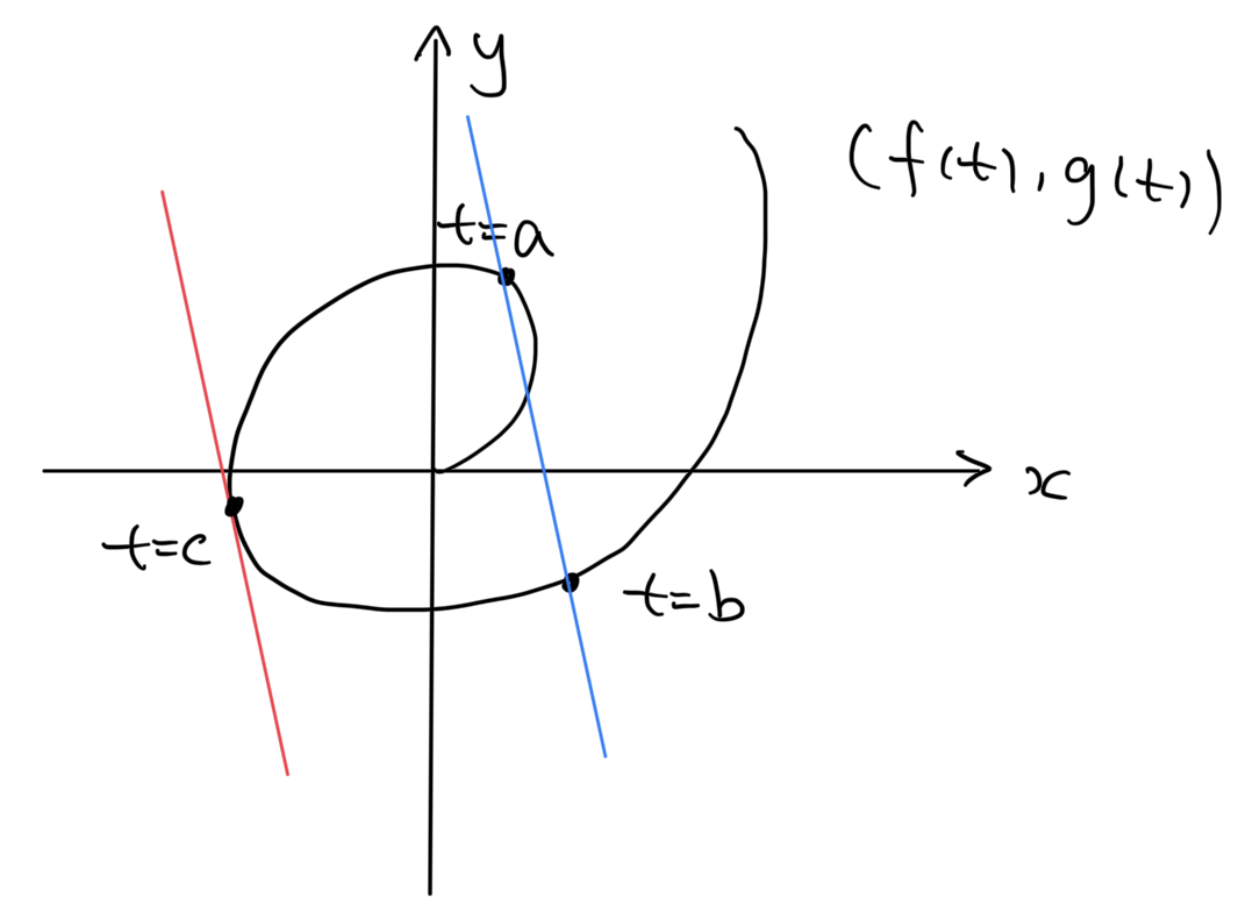
\includegraphics[scale=0.5]{fig/cauchy-mvt.png}
    \caption{Cauchy Mean Value Theorem}
    \label{fig:cauchy-mvt}
\end{figure}

The proof strategy is similar -- we aim to reduce this to \autoref{thm:rolle} (Rolle's Theorem).

\begin{proof}
    Let the function be
    \[
        \phi\pqty{x} = \bqty{g\pqty{x} - g\pqty{a}} \bqty{f\pqty{b} - f\pqty{a}} - \bqty{g\pqty{b} - g\pqty{a}} \bqty{f\pqty{x} - f\pqty{a}}.
    \]

    Note that
    \[
        \phi'\pqty{x} = g'\pqty{x} \pqty{f\pqty{b} - f\pqty{a}} - f'\pqty{x} \pqty{g\pqty{b} - g\pqty{a}},
    \]
    and we have
    \[
        \phi\pqty{a} = \phi\pqty{b} = 0.
    \]

    Applying \autoref{thm:rolle} (Rolle's Theorem) finishes the proof.
\end{proof}

\begin{theorem}[L'H\^{o}pital's Rule]
    \label{thm:l-hopitals}%
    Let \(\minusinfty \leq a < b \leq \plusinfty\). Let \(\functiondomain{f, g}{\oointv{a}{b}}{\RR}\) be differentiable, and \(g'\pqty{x} \neq 0\) for all \(x \in \oointv{a}{b}\). Suppose:
    \begin{itemize}
        \item the limit
        \[
            \lim_{x \to a} \frac{f'\pqty{x}}{g'\pqty{x}} = l
        \]
        exists, where \(l \in \RR \cup \Bqty{\pminfty}\) could be infinite;
        \item \(\lim_{x \to a} f\pqty{x} = \lim_{x \to a} g\pqty{x} = 0\); or \(\lim_{x \to a} g\pqty{x} = \pminfty\).
    \end{itemize}

    Then we have
    \[
        \lim_{x \to a} \frac{f\pqty{x}}{g\pqty{x}} = l.
    \]
\end{theorem}

\begin{proof}
    \textbf{\(\frac{0}{0}\) Case.} We may set \(f\pqty{a} = g\pqty{a} = 0\) in this case. We first note that \(g\pqty{x} \neq 0\). If so, then Rolle's theorem would imply that \(g'\pqty{t} = 0\) for some \(t\) between \(a\) and \(x\).

    By \autoref{thm:cauchy-mvt} (Cauchy's Mean Value Theorem), for any \(x \in \oointv{a}{b}\), there is some \(c\pqty{x} \in \oointv{a}{x}\), such that
    \[
        \frac{f'\pqty{c\pqty{x}}}{g'\pqty{c\pqty{x}}} = \frac{f\pqty{x} - f\pqty{a}}{g\pqty{x} - g\pqty{a}} = \frac{f\pqty{x}}{g\pqty{x}}.
    \]

    We have \(c\pqty{x} \to a\) as \(x \to a\), with \(c\pqty{x} \neq a\). Now, if we have
    \[
        \lim_{x \to a} \frac{f'\pqty{x}}{g'\pqty{x}} = l,
    \]
    then we have
    \[
        \lim_{x \to a} \frac{f'\pqty{c\pqty{x}}}{g'\pqty{c\pqty{x}}} = l,
    \]
    and hence
    \[
        \lim_{x \to a} \frac{f\pqty{x}}{g\pqty{x}} = l
    \]
    as desired.

    \textbf{\(\frac{?}{\infty}\) Case.} This case is mostly similar. We may first restrict the domain such that \(g\pqty{x} \neq 0\) anywhere. Let \(\epsilon > 0\) be arbitrary. Since \(\lim_{x \to a} \frac{f'\pqty{x}}{g'\pqty{x}} = l\), we have some \(\delta\pqty{\epsilon} > 0\), such that
    \[
        \forall x \in \oointv{a}{a + \delta}: \abs{\frac{f'\pqty{x}}{g'\pqty{x}} - l} < \epsilon.
    \]
    
    We fix \(d \in \oointv{a}{a + \delta}\) such that \(g\pqty{d}\) takes the same sign as \(\lim_{x \to a} g\pqty{x}\). For any \(x \in \oointv{a}{d}\), applying \autoref{thm:cauchy-mvt} (Cauchy's Mean Value Theorem), there is some \(c\pqty{x} \in \oointv{x}{d}\), such that
    \[
        \frac{f'\pqty{c\pqty{x}}}{g'\pqty{c\pqty{x}}} = \frac{f\pqty{x} - f\pqty{d}}{g\pqty{x} - g\pqty{d}}.
    \]

    Since \(c\pqty{x} \in \oointv{x}{d}\), we have \(c\pqty{x} \in \oointv{a}{a + \epsilon}\). Therefore, we have
    \[
        \abs{\frac{f\pqty{x} - f\pqty{d}}{g\pqty{x} - g\pqty{d}} - l} < \epsilon.
    \]

    Dividing top and bottom by \(g\pqty{x}\), we have
    \[
        \abs{\frac{\frac{f\pqty{x}}{g\pqty{x}} - \frac{f\pqty{d}}{g\pqty{x}}}{1 - \frac{g\pqty{d}}{g\pqty{x}}} - l} < \epsilon.
    \]

    This implies
    \[
        \abs{1 - \frac{g\pqty{d}}{g\pqty{x}}} \pqty{l - \epsilon} < \frac{f\pqty{x}}{g\pqty{x}} - \frac{f\pqty{d}}{g\pqty{x}} < \abs{1 - \frac{g\pqty{d}}{g\pqty{x}}} \pqty{l + \epsilon}.
    \]

    Therefore, taking \(x \to a\), we have
    \[
        l - \epsilon \leq \liminf_{x \to a} \frac{f\pqty{x}}{g\pqty{x}} \leq \limsup_{x \to a} \frac{f\pqty{x}}{g\pqty{x}} \leq l + \epsilon
    \]
    and taking \(\epsilon \to 0\) gives the desired result. (The final two lines could be replaced with more elementary \(\epsilon-\delta\)s, but I am just not bothered to do that.)
\end{proof}

\begin{example}[Application of L'H\^{o}pital's Rule]
    \label{ex:l-hopitals}%
    We have seen in \autoref{ex:sin-x-x-limit} that
    \[
        \lim_{x \to 0} \frac{\sin x}{x} = 1.
    \]

    L'H\^{o}pital's Rule tells us that
    \[
        \lim_{x \to 0} \frac{\sin x}{x} = \lim_{x \to 0} \frac{\cos x}{1} = 1.
    \]

    Behind the scenes in the rule, we have for some \(\theta \in \oointv{0}{1}\), that
    \[
        \frac{\sin x}{x} = \frac{\sin x - \sin 0}{x - 0} = \frac{\cos \pqty{\theta x}}{1}.
    \]
    
    Then we have
    \[
        \lim_{x \to 0} \frac{\sin x}{x} = \lim_{x \to 0} \cos \pqty{\theta x} = 1.
    \]
\end{example}

Similar to \autoref{ex:inverse-fn-differentiation}, we also have a statement about a \emph{local} function inverse.

\begin{proposition}[Local Inverse Function Theorem]
    \label{prop:local-ivt}%
    Let \(\functiondomain{f}{\ccintv{a}{b}}{\RR}\) be continuous on \(\ccintv{a}{b}\) and continuously differentiable on \(\oointv{a}{b}\). Suppose there is some \(x_0 \in \oointv{a}{b}\) such that \(f'\pqty{x_0} \neq 0\). Then there exists some \(\epsilon > 0\) with \(\ccintv{x_0 - \epsilon}{x_0 + \epsilon} \subseteq \oointv{a}{b}\) such that the restriction
    \[
        \functiondomain{f}{\oointv{x_0 - \epsilon}{x_0 + \epsilon}}{f\pqty{\oointv{x_0 - \epsilon}{x_0 + \epsilon}}}
    \]
    is bijective, and \(f\inverse\) is differentiable with derivative
    \[
        \pqty{f\inverse}'\pqty{y} = \frac{1}{f'\pqty{f\inverse\pqty{y}}}
    \]
    for all \(y \in f\pqty{\oointv{x_0 - \epsilon}{x_0 + \epsilon}}\).
\end{proposition}

\begin{proof}
    Since \(f\) is continuously differentiable, we have \(f'\) is continuous, so there is some neighbourhood about \(x_0\) in \(\oointv{a}{b}\), say \(\ccintv{x_0 - \epsilon}{x_0 + \epsilon}\), such that \(f'\pqty{x} > 0\) for all \(x\) in this interval. Then applying the \autoref{thm:inverse-fn-thm-differentiable} (Inverse Function Theorem for Differentiability) over this interval gives the result as desired.

    Concretely, to show such interval exist, we apply the definition of continuity on \(f'\) near \(x_0\). Take \(\epsilon = f'\pqty{x_0}\), then there is some \(\delta > 0\) such that
    \[
        \forall x \in \ccintv{a}{b}, \abs{x - x_0} < \delta: \abs{f'\pqty{x} - f'\pqty{x_0}} < f'\pqty{x_0}
    \]
    and hence, in particular,
    \[
        \forall x \in \ccintv{a}{b}, \abs{x - x_0} < \delta: f'\pqty{x} > 0.
    \]

    Now, note \(m = \min\Bqty{\delta, x_0 - a, b - x_0} > 0\), so take any \(0 < \epsilon < m\), then for all \(x \in \ccintv{x_0 - \epsilon}{x_0 + \epsilon}\), we have \(x_0 \in \ccintv{a}{b}\) and \(\abs{x - x_0} < \delta\), so \(f'\pqty{x} > 0\) for this restriction.
\end{proof}

\subsection{Darboux's Theorem}

A really cool application of \autoref{thm:extreme-value} (Extreme Value Theorem), \autoref{thm:mean-value-thm} (Mean Value Theorem) and \autoref{thm:intermediate-value} (Intermediate Value Theorem) is the following theorem.

\begin{theorem}[Darboux's Theorem]
    If \(\functiondomain{f}{\ccintv{a}{b}}{\RR}\) is differentiable with \(a < b\), then for all \(f'\pqty{a} < z < f'\pqty{b}\) or \(f'\pqty{b} < z < f'\pqty{a}\), there exists some \(c\) with \(a < c < b\), such that \(f'\pqty{c} = z\).
\end{theorem}

\begin{proof}[\proofname\ using \autoref{thm:extreme-value} (Extreme Value Theorem)]
    We assume that \(f'\pqty{a} < z < f'\pqty{b}\) and the other case is similar. We define the function \(\functiondomain{\phi}{\ccintv{a}{b}}{\RR}\) with
    \[
        \phi\pqty{x} = f\pqty{x} - zx.
    \]

    Since \(f\) is differentiable, it must be continuous, and by \autoref{thm:extreme-value} (Extreme Value Theorem), \(\phi\) attains its bounds.

    Let \(m \in \ccintv{a}{b}\) be such that
    \[
        \phi\pqty{m} = \inf_{x \in \ccintv{a}{b}} \phi\pqty{x}.
    \]

    First, if \(m = a\), then \(\phi\pqty{a} \leq \phi\pqty{x}\) for all \(x \in \ocintv{a}{b}\). Hence, we have
    \[
        f\pqty{a} - az \leq f\pqty{x} - xz.
    \]

    Rearranging, we have
    \[
        z \leq \frac{f\pqty{x} - f\pqty{a}}{x - a}
    \]
    and taking \(x \to a\) gives \(z \leq f'\pqty{a}\), which is a contradiction with \(z > f'\pqty{a}\). So \(m \neq a\)

    Similarly, \(m \neq b\), so \(m \in \oointv{a}{b}\).

    Hence, for any \(x \in \cointv{a}{m}\), we have \(\phi\pqty{x} \geq \phi\pqty{m}\) but \(x - m < 0\), so
    \[
        \frac{\phi\pqty{x} - \phi\pqty{m}}{x - m} \leq 0,
    \]
    and hence in the limit (the limit exists, since \(f\) is differentiable implies \(\phi\) is differentiable),
    \[
        \phi'\pqty{m} \leq 0.
    \]

    Similarly, considering \(x \in \ocintv{m}{b}\), we have \(\phi'\pqty{m} \geq 0\). So \(\phi'\pqty{m} = 0\), and hence \(f'\pqty{m} = z\), finishing our proof.
\end{proof}

\begin{proof}[\proofname\ using \autoref{thm:mean-value-thm} (Mean Value Theorem) and \autoref{thm:intermediate-value} (Intermediate Value Theorem)]
    We consider the helper functions
    \[
        g\pqty{x} = \begin{cases}
            f'\pqty{a}, & x = a, \\
            \frac{f\pqty{x} - f\pqty{a}}{x - a}, & a < x \leq b,
        \end{cases}
    \]
    and
    \[
        h\pqty{x} = \begin{cases}
            \frac{f\pqty{x} - f\pqty{b}}{x - b}, & a \leq x < b, \\
            f'\pqty{b}, & x = b.
        \end{cases}
    \]

    Now, note that
    \[
        g\pqty{b} = h\pqty{a} = \frac{f\pqty{a} - f\pqty{b}}{a - b}.
    \]

    Hence, for \(f'\pqty{a} < z < f'\pqty{b}\), it must lie within either the image of \(g\), or the image of \(h\), since \(g\) and \(h\) are both continuous, and by \autoref{thm:intermediate-value} (Intermediate Value Theorem). In the first case,
    \[
        z = \frac{f\pqty{t} - f\pqty{a}}{t - a}
    \]
    for some \(a < t \leq b\), and in the second case,
    \[
        z = \frac{f\pqty{t} - f\pqty{b}}{t - b}
    \]  
    for some \(a \leq t < b\). Either case, we have
    \[
        z = \frac{f\pqty{\alpha} - f\pqty{\beta}}{\alpha - \beta}
    \]
    for \(\ccintv{\alpha}{\beta} \subseteq \ccintv{a}{b}\).

    Therefore, by \autoref{thm:mean-value-thm} (Mean Value Theorem), we have
    \[
        z = f' \pqty{c}  
    \]
    for some \(\alpha < c < \beta\), and hence for some \(a < c < b\).
\end{proof}

\subsection{Higher Derivatives and Taylor's Theorem}
\begin{definition}[Higher Order Derivatives]
    \label{def:higher-order-derivatives}%
    Suppose \(\functiondomain{f}{X \subseteq \CC}{\CC}\) is differentiable on \(X\). We say the function \(f\) is \term{twice differentiable} on \(X\), if
    \[
        \function{f'}{X}{\CC}{x}{f'\pqty{x}}
    \]
    is differentiable. We define \(f\) is \term{\(k\)-times differentiable} similarly, and denote this as \(f \in \diffClass{k} \pqty{X}\).

    We say \(f\) is \term{\(k\)-times continuously differentiable}, and denote this as \(f \in \contClass{k} \pqty{X}\), if \(f\) is \(k\)-times differentiable and the \(k\)-th derivative
    \[
        \function{f^{\pqty{k}}}{X}{\CC}{x}{f^{\pqty{k}}\pqty{x}}
    \]
    is continuous.
\end{definition}

Note that the function spaces (differentiability classes) have the following containment relationship.
\[
    \contClass{0}\pqty{X} \supset \diffClass{1}\pqty{X} \supset \contClass{1}\pqty{X} \supset \diffClass{2}\pqty{X} \supset \contClass{2}\pqty{X} \supset \cdots,
\]
and that note these are strict inclusions.

\begin{definition}[Smooth]
    \label{def:smooth}%
    We say \(\functiondomain{f}{X}{\CC}\) is \term{smooth} if \(f \in \diffClass{k}\pqty{X}\) for all \(k \in \NN\), and we denote this as
    \[
        f \in \smoothClass \pqty{X}.
    \]
\end{definition}

We saw from \autoref{lem:linear-approximation-differentiability} that \(f\) differentiable at \(a\) means \(f\) can be well-approximated by a linear function near \(a\), by
\[
    f\pqty{x} \approx f\pqty{a} + f'\pqty{a} \pqty{x - a}.
\]

Similarly, we may have
\[
    f\pqty{x} \approx f\pqty{a} + f'\pqty{a} \pqty{x - a} + \frac{1}{2} f''\pqty{a} \pqty{x - a}^2
\]
and in fact if it is \(n\)-times differentiable, we have
\[
    f\pqty{x} \approx \sum_{k = 0}^{n} \frac{f^{\pqty{k}} \pqty{a}}{k!} \cdot \pqty{x - a}^{k}.
\]

We want to quantify how correct this approximation is -- i.e., we want to quantify the \emph{remainder}.

\begin{definition}[Taylor Polynomial, Taylor Series]
    \label{def:taylor-polynomial-series}%
    If \(\functiondomain{f}{X}{\CC}\) is \(n\)-times differentiable at \(x_0 \in X\), then for \(x_0 + h \in X\), the \term{Taylor Polynomial} of degree \(n\) at \(x_0\) is defined as
    \[
        T_{n, f, x_0} \pqty{h} = \sum_{k = 0}^{n} \frac{f^{\pqty{k}} \pqty{x_0}}{k!} \cdot h^{k}.
    \]

    If \(f\) is smooth at \(x_0 \in X\), then the infinite series
    \[
        \sum_{k = 0}^{\infty} \frac{f^{\pqty{k}} \pqty{x_0}}{k!} \cdot h^{k}
    \]
    is the \term{Taylor Series} of \(f\) at \(x_0\).
\end{definition}

We will see different versions of Taylor's Theorems, all of which aims to quantify what the remainder is, but giving it in different forms.

\begin{definition}[Taylor Remainder]
    Suppose \(\functiondomain{f}{X}{\CC}\) is \(\pqty{n - 1}\)-times differentiable at \(a \in X\). Then for \(h \in X\), we let
    \[
        R_{n, f, a} \pqty{h} = f\pqty{a + h} - T_{n - 1, f, a} \pqty{h} = f\pqty{a + h} - \sum_{k = 0}^{n - 1} \frac{f^{\pqty{k}} \pqty{a}}{k!} \cdot h^k
    \]
    be the \term{Taylor remainder}.
\end{definition}

\subsubsection{Mean Value Forms of the Remainder}

\begin{theorem}[Taylor's Theorem with Lagrange Remainder]
    \label{thm:taylor-thm-langrange-remainder}%
    Let \(\functiondomain{f}{\ccintv{a}{a + h}}{\RR}\) be \(n\) times differentiable on \(\oointv{a}{a + h}\) and \(\pqty{n - 1}\) times continuously differentiable on \(\ccintv{a}{a + h}\). Then the \term{Lagrange Form of the Remainder} gives the Taylor remainder in the form
    \[
        R_{n, f, a} \pqty{h} = \frac{h^n}{n!} \cdot f^{\pqty{n}} \pqty{a + \theta h},
    \]
    for some \(\theta \in \oointv{0}{1}\).
\end{theorem}

\begin{remarks}
    \begin{itemize}
        \item When \(n = 1\), this simply gives \autoref{thm:mean-value-thm} (Mean Value Theorem).
        \item Furthermore, there is nothing special about \(h > 0\): we could simply swap the bounds of the intervals (i.e. \(\ccintv{a}{a + h}\) to \(\ccintv{a + h}{a}\) and \(\oointv{a}{a + h}\) to \(\oointv{a + h}{a}\)), and we will still get a similar result.
        \item If \(f \in \contClass{n} \pqty{\oointv{c}{d}}\) with \(\ccintv{a}{a + h} \subset \oointv{c}{d}\), then note that \(f^{\pqty{n}}\) is continuous on the closed interval, hence bounded, and let
        \[
            M_n = \sup_{x \in \ccintv{a}{a + h}} \abs{f^{\pqty{n}} \pqty{x}}.
        \]

        Then
        \[
            \abs{R_{n, f, a} \pqty{h}} \leq M_n \cdot \frac{\abs{h}^n}{n!}
        \]
        and we have \(R_{n, f, a} \pqty{h} = \bigO \pqty{h^n}\) as \(h \to 0\), or in other words, the approximation gets better as the point \(a + h\) gets closer to \(a\). \textbf{However, this does not tell us that \(R_{n, f, a} \pqty{h} \to 0\) as \(n \to \infty\)}, or in other words, adding more terms does not necessarily make our approximation better. Even if \(f \in \smoothClass\), we still do not know how \(M_n\) behaves with \(n\). (In other words, there are smooth functions that are not analytic (on \(\RR\)).)
    \end{itemize}
\end{remarks}

\begin{proof}[\proofname\ (First Proof)]
    Without loss of generality, we let \(a = 0\). Let
    \[
        \function{\phi}{\ccintv{0}{h}}{\RR}{t}{f\pqty{t} - T_{n - 1, f, 0} \pqty{t} - \frac{t^n}{n!} \cdot B}
    \]
    where we pick the constant \(B\) such that \(\phi\pqty{h} = 0\). Note that \(\phi\) is continuous, and that its \(\pqty{n - 1}\)-th derivatives is continuous on \(\ccintv{0}{h}\) and its \(n\)-th derivatives exists on \(\oointv{0}{h}\). Note that \(\phi\pqty{0} = 0\) and also \(\phi^{\pqty{k}} \pqty{0} = 0\) for all \(k = 0, \ldots, n - 1\).

    Since we have
    \[
        \phi\pqty{0} = \phi\pqty{h} = 0,
    \] 
    by \autoref{thm:rolle} (Rolle's Theorem), we have some \(\theta_1 \in \oointv{0}{1}\) with \(\phi'\pqty{\theta_1 h} = 0\). Applying Rolle's Theorem again on the interval \(\ccintv{0}{\theta_1 h}\) with the function \(\phi'\), we have some \(\theta_2 \in \oointv{0}{1}\) with \(\phi''\pqty{\theta_2 \theta_1 h} = 0\).

    Hence, by induction, we have some \(\theta_1, \theta_2, \ldots, \theta_n \in \oointv{0}{1}\), such that
    \[
        \phi^{\pqty{n}} \pqty{\theta_n \theta_{n - 1} \cdots \theta_{2} \theta_{1} h} = 0.
    \]

    We set \(\theta = \theta_n \theta_{n - 1} \cdots \theta_{2} \theta_{1} \in \oointv{0}{1}\), and hence there exists some \(\theta \in \oointv{0}{1}\), such that
    \[
        f^{\pqty{n}} \pqty{t} - B = \phi^{\pqty{n}} \pqty{\theta h} = 0,
    \]
    and hence
    \[
        B = f^{\pqty{n}} \pqty{\theta h},
    \]
    is indeed an error term, as desired.
\end{proof}

The first proof almost certainly much easier than the proof below, but this proof generalises the remainder into a more general case, which would be introduced in \autoref{thm:taylor-thm-cauchy-remainder} (Cauchy Form) and \autoref{thm:taylor-thm-schlomilch-remainder} (Schl\"{o}milch Form).

\begin{proof}[\proofname\ (Second Proof)]
    Without loss of generality, set \(a = 0\). Let
    \[
        \function{g}{\ccintv{0}{h}}{\RR}{t}{f\pqty{h} - \sum_{k = 0}^{n - 1} \frac{f^{\pqty{k}} \pqty{t}}{k!} \cdot \pqty{h - t}^{k}.}
    \]

    Note that
    \[
        g\pqty{0} = f\pqty{h} - T_{n - 1, f, 0} \pqty{h}.
    \]  

    Note \(g\) is continuous on \(\ccintv{0}{h}\) and differentiable on \(\oointv{0}{h}\), with
    \[
        g'\pqty{t} = - \frac{f^{\pqty{n}}\pqty{t}}{\pqty{n - 1}!} \pqty{h - t}^{n - 1}.
    \]

    Therefore, for any \(p > 0\), set
    \[
        \phi_{p} \pqty{t} = g\pqty{t} - \frac{\pqty{h - t}^{p}}{h^p} g\pqty{0}.
    \]

    We may verify that \(\phi_{p} \pqty{h} = \phi_p \pqty{0} = 0\). Hence, by \autoref{thm:rolle} (Rolle's Theorem), there is some \(\theta \in \oointv{0}{1}\) such that
    \[
        \phi_p' \pqty{\theta h} = g' \pqty{\theta h} + \frac{p \pqty{h - \theta h}^{p - 1}}{h^p} \cdot g\pqty{0} = g'\pqty{\theta h} + \frac{p \pqty{1 - \theta}^{p - 1}}{h} \cdot g\pqty{0} = 0.
    \]

    Therefore, there is some \(\theta \in \oointv{0}{1}\), such that
    \[
        - \frac{h^{n - 1} \pqty{1 - \theta}^{n - 1}}{\pqty{n - 1}!} \cdot f^{\pqty{n}} \pqty{\theta h} + p \cdot \frac{\pqty{1 - \theta}^{p - 1}}{h} \cdot g\pqty{0} = 0.
    \]

    Hence, by rearranging, we have
    \[
        f\pqty{h} - T_{n - 1, f, 0} \pqty{h} = \frac{h^n}{p \pqty{n - 1}!} \pqty{1 - \theta}^{n - p} \cdot f^{\pqty{n}} \pqty{\theta h}.
    \]

    We take \(p = n\), and we have the result as desired.
\end{proof}

Although the second proof looks very horrible, this in fact gives another version of Taylor's theorem, with a different estimate -- since we can choose all \(p\)s!

\begin{theorem}[Taylor's Theorem with Cauchy Remainder]
    \label{thm:taylor-thm-cauchy-remainder}%
    Let \(\functiondomain{f}{\ccintv{a}{a + h}}{\RR}\) be \(n\) times differentiable on \(\oointv{a}{a + h}\) and \(\pqty{n - 1}\) times continuously differentiable on \(\ccintv{a}{a + h}\). Then the \term{Cauchy Form of the Remainder} gives the Taylor remainder in the form
    \[
        R_{n, f, a} \pqty{h} = \frac{h^{n}}{\pqty{n - 1}!} \cdot \pqty{1 - \theta}^{n - 1} f^{\pqty{n}} \pqty{a + \theta h},
    \]
    for some \(\theta \in \oointv{0}{1}\).
\end{theorem}

\begin{proof}
    By putting \(p = 1\) into the second proof of \autoref{thm:taylor-thm-langrange-remainder}.
\end{proof}

\begin{remark}
    Similarly, if we have \(f \in \contClass{n} \pqty{\oointv{c}{d}}\) with \(\ccintv{a}{a + h} \subset \oointv{c}{d}\), then as in previous remark, we may set
    \[
        M_n = \sup_{x \in \ccintv{a}{a + h}} \abs{f^{\pqty{n}} \pqty{x}}
    \]
    and by \autoref{thm:taylor-thm-cauchy-remainder}, then we have
    \[
        \abs{R_{n, f, a} \pqty{h}} \leq M_n \cdot \frac{\abs{h}^n}{\pqty{n - 1}!}.
    \]
\end{remark}

This looks like an even worse estimate, since \(\pqty{n - 1}!\) on the denominator gives a bigger error than \(\pqty{n}!\). However, this is not necessarily true -- as the following example will demonstrate.

\begin{example}[Application of Taylor's Theorems]
    \label{ex:application-taylor}%
    Consider the function \(f\pqty{x} = x^q\) for some rational \(q \in \QQ\). This function is smooth on \(\oointv{0}{\plusinfty}\). We may attempt to calculate its derivates by
    \[
        f^{\pqty{k}} \pqty{x} = q \cdot \pqty{q - 1} \cdot \pqty{q - 2} \cdots \pqty{q - k + 1} \cdot x^{q - k}.
    \]

    We may calculate the Taylor polynomial at \(1\) as
    \[
        T_{n - 1, f, 1} \pqty{h} = \sum_{k = 0}^{n - 1} \frac{q \pqty{q - 1} \cdots \pqty{q - k + 1}}{k!} \cdot h^k = \sum_{k = 0}^{n - 1} \binom{q}{k} h^k.
    \]

    We now look at
    \[
        R_{n, f, 1} \pqty{h} = \pqty{1 + h}^{q} - \sum_{k = 0}^{n - 1} \binom{q}{k} h^k
    \]
    in \(\oointv{-1}{1}\). In particular, we would like to study if the remainder converges to \(0\) as \(n \to \infty\). (This is trivial for \(h = 0\).)

    We evaluate both remainders. If we use \autoref{thm:taylor-thm-langrange-remainder} (Lagrange Remainder), we have some \(\theta \in \oointv{0}{1}\) such that
    \[
        R_{n, f, 1} \pqty{h} = \binom{q}{n} \pqty{1 + \theta h}^{q - n} h^n.
    \]

    If \(n \geq q\), then \(\pqty{1 + \theta h}^{q - n} \leq 1\) for \(h \in \cointv{0}{1}\), and hence
    \[
        \abs{R_{n, f, 1} \pqty{h}} \leq \abs{\binom{q}{n} h^n} \to 0
    \]
    as \(n \to \infty\), for any \(h \in \cointv{0}{1}\). However, this argument fails for \(h \in \oointv{-1}{0}\).

    If we use \autoref{thm:taylor-thm-cauchy-remainder} (Cauchy Remainder), we have some \(\theta \in \oointv{0}{1}\) (not necessarily identical to the \(\theta\) before), that
    \begin{align*}
        R_{n, f, 1} \pqty{h} &= \binom{q}{n} \cdot n \cdot \pqty{1 - \theta}^{n - 1} \cdot \pqty{1 + \theta h}^{q - n} \cdot h^n \\
        &= \pqty{1 - \theta}^{n - 1} q \binom{q - 1}{n - 1} \pqty{1 + \theta h}^{q - n} h^n \\
        &= q \binom{q - 1}{n - 1} \cdot \pqty{\frac{1 - \theta}{1 + \theta h}}^{n - 1} \cdot \pqty{1 + \theta h}^{q - 1} h^n.
    \end{align*}

    Now, for any \(h \in \oointv{-1}{1}\), we have \(1 + \theta h = \pqty{1 - \theta} + \theta \pqty{h + 1} \geq 1 - \theta\). Hence, we have
    \[
        \pqty{\frac{1 - \theta}{1 + \theta h}}^{n - 1} \leq 1
    \]
    as long as \(n \geq 1\). Hence, we may apply a bound the remainder by
    \[
        \abs{R_{n, f, 1} \pqty{h}} \leq \abs{qh} \cdot \abs{\binom{q - 1}{n - 1} h^{n - 1}} \cdot \abs{1 + \theta h}^{q - 1}.
    \]

    Note that only the middle term depends on \(n\). Therefore,
    \[
        \abs{R_{n, f, 1} \pqty{h}} \to 0
    \]
    as \(n \to \infty\) for every \(h \in \oointv{-1}{1}\).
    
    So the Cauchy remainder gives us that the remainder is exponentially small as \(n \to \infty\), for all \(h \in \oointv{-1}{1}\), while the Lagrange remainder only guaranteed that for the range of \(h \in \cointv{0}{1}\).
\end{example}

\begin{definition}[Analytic Function]
    \label{def:analytic}%
    We say that \(f \in \smoothClass \pqty{\oointv{c}{d}}\) is \term{analytic}, denoted as \(f \in \analyticClass \pqty{\oointv{c}{d}}\), if for every \(a \in \oointv{c}{d}\), there exists an \(r > 0\), such that for all \(\abs{h} < r\),
    \[
        f\pqty{a + h} = \sum_{k = 0}^{\infty} \frac{f^{\pqty{k}} \pqty{a}}{k!} \cdot h^k = \lim_{n \to \infty} T_{n, f, a} \pqty{h}.
    \]

    Equivalently, we have
    \[
        \lim_{n \to \infty} R_{n, f, a} \pqty{h} = 0.
    \]

    In other words, analytic functions are functions whose Taylor series at any point converges to the function within some non-zero radius.
\end{definition}

\begin{example}[Analytic Function]
    \label{ex:analytic-fn}%
    As in \autoref{ex:application-taylor}, the function \(x^q\) is analytic in \(\oointv{0}{2}\) -- in other words, \(\pqty{1 + x}^q\) is analytic in \(\oointv{-1}{1}\).
\end{example}

\begin{remark}
    Even if \(R_{n, f, a} \pqty{h} \notto 0\) as \(n \to \infty\), this \emph{does not mean} that the Taylor series
    \[
        \sum_{k = 0}^{\infty} \frac{f^{\pqty{k}} \pqty{a}}{k!} \cdot h^k
    \]
    does not converge -- it just means that the Taylor series does not converge to the actual function value. (In \(\RR\), there are smooth functions that are not analytic.)
\end{remark}

Finally, just for completeness, we introduce the name for the general form when we do not specify the value of \(p\).

\begin{theorem}[Taylor's Theorem with Schl\"{o}milch Remainder]
    \label{thm:taylor-thm-schlomilch-remainder}%
    Let \(\functiondomain{f}{\ccintv{a}{a + h}}{\RR}\) be \(n\) times differentiable on \(\oointv{a}{a + h}\) and \(\pqty{n - 1}\) times continuously differentiable on \(\ccintv{a}{a + h}\). Then the \term{Schl\"{o}milch Form of the Remainder} gives the Taylor remainder in the form, for any fixed \(p > 0\),
    \[
        R_{n, f, a} \pqty{h} = \frac{h^{n}}{p \pqty{n - 1}!} \cdot \pqty{1 - \theta}^{n - p} f^{\pqty{n}} \pqty{a + \theta h},
    \]
    for some \(\theta \in \oointv{0}{1}\).
\end{theorem}

\begin{proof}
    Identical to the second proof of \autoref{thm:taylor-thm-langrange-remainder}.
\end{proof}

\subsubsection{Asymptotic Form of the Remainder}

This section is not mentioned in the lecture, but I think it just really makes sense to include it here.

A good question to ask is, must the Taylor polynomial be correct up to its degree? Is there a better degree-\(n\) polynomial that fits the function better?

\begin{theorem}[Taylor's Theorem with Peano Remainder]
    \label{thm:taylor-thm-peano-remainder}%
    Let \(\functiondomain{f}{\oointv{c}{d}}{\RR}\) be \(\pqty{n - 1}\) times differentiable. Then for any \(a \in \oointv{c}{d}\), the \term{Peano Form of the Remainder} gives the Taylor remainder in the form
    \[
        R_{n, f, a} \pqty{h} = \littleO\pqty{h^{n - 1}}.
    \]
\end{theorem}

\begin{proof}
    We may show this by induction on \(n\), and using \autoref{thm:l-hopitals} (L'H\^{o}pital's Rule). Without loss of generality, let \(a = 0\). Recall from the definition of the little-\(\littleO\) notation, that we want to show
    \[
        \lim_{h \to 0} \frac{R_{n, f, 0} \pqty{h}}{h^{n - 1}} = 0.
    \]

    The base case where \(n = 1\) is trivial, and for \(n = 2\) is proven in \autoref{lem:linear-approximation-differentiability}.

    For the general case, recall that
    \[
        R_{n, f, 0} \pqty{h} = f\pqty{h} - \sum_{k = 0}^{n - 1} \frac{f^{\pqty{k}} \pqty{0}}{k!} \cdot h^k.
    \]

    Since \(f\) is \(\pqty{n - 1}\) times differentiable at \(0\), we have \(R\) is \(\pqty{n - 1}\) times differentiable at \(0\), and in particular, continuous. Hence,
    \[
        \lim_{h \to 0} R_{n, f, 0} \pqty{h} = R_{n, f, 0} \pqty{0} = 0.
    \]
    
    Therefore, this satisfies the setup of L'H\^{o}pital's Rule, and hence we calculate the derivative of \(R_{n, f, a} \pqty{h}\). We note
    \[
        R'_{n, f, 0} \pqty{h} = f'\pqty{h} - \sum_{k = 1}^{n - 1} \frac{f^{\pqty{k}} \pqty{0}}{\pqty{k - 1}!} \cdot h^{k - 1} = f'\pqty{h} - \sum_{k = 0}^{n - 2} \frac{f^{\pqty{k + 1}} \pqty{0}}{k!} \cdot h^k = R_{n - 1, f', 0} \pqty{h}.
    \]

    Therefore, it suffices to show for \(f'\) (which is \(\pqty{n - 2}\) times differentiable), that
    \[
        R_{n - 1, f', 0} \pqty{h} = \littleO\pqty{h^{n - 2}}.
    \]

    This is indeed true by our induction hypothesis.
\end{proof}

This result shows that the remainder term must have strictly higher order than \(h^{n - 1}\), and hence Taylor's Polynomial is indeed the best \(n\)-th order polynomial we can get, in the asymptotic sense.
\section{Integration of Functions}

\subsection{Basics}

\subsubsection{Definition of Riemann Sums and Integrals}

We have learnt before that the integral
\[
    \int_{a}^{b} f\pqty{x} \dd{x}
\]
gives the signed area under the graph of \(f\), for \(\functiondomain{f}{\ccintv{a}{b}}{\RR}\). We now aim to quantify it rigorously.

We may attempt to approximate the function using rectangles -- specifically using rectangles \emph{taller} than the function to \emph{overestimate}, and \emph{lower} than the function to \emph{underestimate}. Ideally, if we make the width of the split smaller and smaller, however we split it, that the overestimate and the underestimate will eventually `converge' to the same limit -- which makes the function \emph{integrable}. (Warning: it is hard to quantify `smaller and smaller'!)

\begin{definition}[Upper and Lower Riemann Sums]
    \label{def:upper-lower-riemann-sum}%
    Let \(\functiondomain{f}{\ccintv{a}{b}}{\RR}\) be bounded. Let a \term{partition/dissection} \(\partition = \Bqty{x_0, x_1, \ldots, x_n}\) with \(a = x_0 < x_1 < \cdots x_n = b\) be given. Then we let
    \[
        \upperSum \pqty{f, \partition} = \sum_{j = 1}^{n} \pqty{\sup_{x \in \ccintv{x_{j - 1}}{x_{j}}} f\pqty{x}} \cdot \pqty{x_j - x_{j - 1}}
    \]
    as the \term{Upper Riemann Sum}, and similarly,
    \[
        \lowerSum \pqty{f, \partition} = \sum_{j = 1}^{n} \pqty{\inf_{x \in \ccintv{x_{j - 1}}{x_{j}}} f\pqty{x}} \cdot \pqty{x_j - x_{j - 1}}
    \]
    as the \term{Lower Riemann Sum}, of the function \(f\) associated to the partition \(\partition\).
\end{definition}

\begin{example}[Riemann Sums]
    \label{ex:riemann-sums}%
    Consider the function
    \[
        f\pqty{x} = \begin{cases}
            1, & x \in \QQ, \\
            0, & x \in \RR \setminus \QQ
        \end{cases}
    \]
    on \(\ccintv{0}{1}\). For any \(\partition\) we take, we will have both rationals and irrationals in \(I_j = \ccintv{x_{j - 1}}{x_j}\), and hence we always have
    \[
        \upperSum \pqty{f, \partition} = 1, \quad \lowerSum \pqty{f, \partition} = 0.
    \]
\end{example}

We assumed that \(f\) is bounded, and say \(\sup_{x \in \ccintv{a}{b}} \abs{f} = k\), then
\begin{align*}
    \upperSum\pqty{f, \partition} &= \sum_{j = 1}^{n} \pqty{\sup_{\ccintv{x_{j - 1}}{x_j}} f} \pqty{x_j - x_{j - 1}} \\
    &\leq \sum_{j = 1}^{n} \pqty{\sup_{\ccintv{a}{b}} f} \pqty{x_j - x_{j - 1}} \\
    &= k \sum_{j = 1}^{n} \pqty{x_j - x_{j - 1}} \\
    &= k \pqty{b - a},
\end{align*}
and similarly,
\[
    \lowerSum\pqty{f, \partition} \geq -k \pqty{b - a}.
\]

Also, we have \(\upperSum\pqty{f, \partition} \geq \lowerSum\pqty{f, \partition}\). Therefore, the sets
\[
    \set{\upperSum\pqty{f, \partition}}{\partition \text{ is a partition of }\ccintv{a}{b}}
\]
and
\[
    \set{\lowerSum\pqty{f, \partition}}{\partition \text{ is a partition of }\ccintv{a}{b}}
\]
are both bounded, non-empty sets.

\begin{definition}[Upper and Lower Integrals]
    \label{def:upper-lower-int}%
    Let \(\functiondomain{f}{\ccintv{a}{b}}{\RR}\) be bounded. We say
    \[
        \upperI \pqty{f} = \upperInt_{a}^{b} f \pqty{x} \dd{x} = \inf_{\partition\text{ is a partition of }\ccintv{a}{b}} \upperSum \pqty{f, \partition}
    \]
    be the \term{upper integral} of \(f\), and similarly,
    \[
        \lowerI \pqty{f} = \lowerInt_{a}^{b} f \pqty{x} \dd{x} = \sup_{\partition\text{ is a partition of }\ccintv{a}{b}} \lowerSum \pqty{f, \partition}
    \]
    be the \term{lower integral} of \(f\).
\end{definition}

Note we actually didn't take a `limit' as the width tends to zero -- that is slightly tougher to formalise (it is possible to do so, as the limit of a mesh), but this works just as well (since narrowing the widths seems to decrease the error, which makes it smaller for overestimates, and larger for underestimates) -- but note because of this, lots of properties of the integral is \textbf{not} a direct consequence of the properties of the limit, which is a common misconception.

\begin{definition}[Riemann Integral]
    \label{def:riemann-integral}%
    We say \(f\) is \term{Riemann Integrable} if \(\upperI \pqty{f} = \lowerI \pqty{f}\), and we denote the \term{Riemann Integral} as
    \[
        I\pqty{f} = \int_{a}^{b} f\pqty{x} \dd{x} = \upperI\pqty{f} = \lowerI\pqty{f}.
    \]
\end{definition}

\begin{remark}
    We define by convention
    \[
        \int_{a}^{b} f = - \int_{b}^{a} f.
    \]
\end{remark}

\begin{example}[Non-Riemann Integrable Function]
    \label{ex:non-riemann-integrable-fn}%
    Continuing from \autoref{ex:riemann-sums}, we note that \(\upperI\pqty{f} = 1\) while \(\lowerI\pqty{f} = 0\). Hence, this function is not Riemann integrable.
    
    Just as a remark, it is Lebesgue integrable using the Lebesgue measure, and the result is \(0\) -- intuitively, there are `way too few' rational numbers (and this is saying \(\QQ\) has zero Lebesgue measure, since it is countable).
\end{example}

The coarsest possible partition for \(\ccintv{a}{b}\) is the partition \(\Bqty{a, b}\). Our intuition is that a finer partition leads to a better estimate for the area.

\begin{lemma}[Refinements provide Better Estimates]
    \label{lem:refinement-better-estimate}%
    Let \(\partition, \partition'\) be two partitions of \(\ccintv{a}{b}\), with \(\partition' \supseteq \partition\) (i.e., \(\partition'\) is a \term{refinement} of \(\partition\)). Then we have
    \[
        \lowerSum\pqty{f, \partition} \leq \lowerSum\pqty{f, \partition'} \leq \upperSum\pqty{f, \partition'} \leq \upperSum\pqty{f, \partition}.
    \]
\end{lemma}

\begin{proof}
    We show this by induction on refining the partition point-by-point.
    
    Take \(\partition = \Bqty{x_0, x_1, \ldots, x_n}\) where \(0 = x_0 < x_1 < \cdots < x_n = b\). Pick \(y \in \oointv{x_{k - 1}}{x_k}\) for some \(k\).

    Set
    \[
        \partition' = \partition \cup \Bqty{y} = \Bqty{x_0, \ldots, x_{k - 1}, y, x_k, \ldots, x_n}.
    \]

    Then, the only change in the sum is the supremum
    \[
        \sup_{x \in \ccintv{x_{n - 1}}{y}} f\pqty{x}, \sup_{x \in \ccintv{y}{x_n}} f\pqty{x} \leq \sup_{x \in \ccintv{x_{n - 1}}{x_n}} f\pqty{x}.
    \]

    Multiplying by the widths, we can see that
    \[
        \pqty{y - x_{k - 1}} \sup_{x \in \ccintv{x_{k - 1}}{y}} f\pqty{x} + \pqty{x_k - y} \sup_{x \in \ccintv{y}{x_k}} f\pqty{x} \leq \pqty{x_k - x_{k - 1}} \sup_{x \in \ccintv{x_{k - 1}}{x_k}} f\pqty{x}.
    \]

    Hence, we have
    \[
        \upperSum\pqty{f, \partition'} \leq \upperSum \pqty{f, \partition}.
    \]

    Similarly, we may show (replacing with infimums and the opposite inequalities), that
    \(
        \lowerSum\pqty{f, \partition'} \geq \lowerSum \pqty{f, \partition}.
    \)

    If \(\partition'\) differs by \(n\) points, we repeat this argument \(n\) times (since partitions are defined to be finite).
\end{proof}

\begin{lemma}[Upper Sums are always at least Lower Sums]
    \label{lem:upper-greater-lower-sum}%
    Let \(\partition\) and \(\partition'\) be partitioned \(\ccintv{a}{b}\) (but not necessarily one being the refinement of the other). Then we have
    \[
        \lowerSum\pqty{f, \partition} \leq \upperSum\pqty{f, \partition'}
    \]
    and similarly
    \[
        \lowerSum\pqty{f, \partition'} \leq \upperSum\pqty{f, \partition}.
    \]
\end{lemma}

\begin{proof}
    We take the common refinement \(\partition \cup \partition'\). Therefore, by \autoref{lem:refinement-better-estimate},
    \[
        \lowerSum\pqty{f, \partition} \leq \lowerSum\pqty{f, \partition \cup \partition'} \leq \upperSum\pqty{f, \partition \cup \partition'} \leq \upperSum\pqty{f, \partition'}.
    \]
\end{proof}

\begin{corollary}[Upper Integrals are always at least Lower Integrals]
    \label{cor:upper-greater-lower-int}%
    We have for any bounded \(\functiondomain{f}{\ccintv{a}{b}}{\RR}\), that
    \[
        \lowerI\pqty{f} = \lowerInt_{a}^{b} f\pqty{x} \dd{x} \leq \upperInt_{a}^{b} f\pqty{x} \dd{x} = \upperI \pqty{f}.
    \]
\end{corollary}

\begin{proof}
    We have \(\lowerSum\pqty{f, \partition} \leq \upperSum\pqty{f, \partition'}\) from \autoref{lem:upper-greater-lower-sum}. Taking the infimum over all \(\partition'\) gives
    \[
        \lowerSum\pqty{f, \partition} \leq \inf_{\partition'} \upperSum\pqty{f, \partition'} = \upperI.
    \]

    Taking the supremum over all \(\partition\) gives
    \[
        \lowerI = \sup_{\partition} \lowerSum\pqty{f, \partition} \leq \upperI
    \]
    as desired.
\end{proof}

Another way of viewing integrability is as follows: we can always find a partition \(\partition\) of \(\ccintv{a}{b}\), such that the upper sum (overestimate) and the lower sum (underestimate) differ by, at most, any arbitrary threshold that we specify.

\begin{proposition}[Riemann Integrability Criteria]
    \label{prop:riemann-integrability-criteria}%
    Let \(\functiondomain{f}{\ccintv{a}{b}}\) be bounded. Then \(f\) is Riemann integrable, if and only if
    \[
        \forall \epsilon > 0, \exists \partition: \upperSum\pqty{f, \partition} - \lowerSum\pqty{f, \partition} < \epsilon,
    \]
    where \(\partition\) is a partition.
\end{proposition}

\begin{proof}
    Suppose that the criteria is true. We have
    \[
        0 \leq \upperI\pqty{f} - \lowerI\pqty{f} \leq \upperSum\pqty{f, \partition} - \lowerSum\pqty{f, \partition} < \epsilon,
    \]
    for any \(\epsilon > 0\), and so we must have \(\upperI\pqty{f} - \lowerI\pqty{f} = 0\).

    Now, suppose that \(f\) is Riemann integrable. By the definition of the supremum and infimum, we can always find partitions \(\partition, \partition'\) such that
    \[
        \upperSum\pqty{f, \partition} \leq \upperI\pqty{f} + \frac{\epsilon}{2}
    \]
    and
    \[
        \lowerSum\pqty{f, \partition'} \geq \lowerI\pqty{f} + \frac{\epsilon}{2}.
    \]

    Therefore,
    \[
        \upperSum\pqty{f, \partition} - \lowerSum\pqty{f, \partition'} \leq \epsilon.
    \]

    To conclude, we take a common refinement \(\partition \cup \partition'\), and then we have
    \[
        \upperSum\pqty{f, \partition \cup \partition'} - \lowerSum\pqty{f, \partition \cup \partition'} \leq \upperSum\pqty{f, \partition} - \lowerSum\pqty{f, \partition'} \leq \epsilon,
    \]
    so we are done.
\end{proof}

Note that this is equivalent to the following sequential version.

\begin{proposition}[Sequential Riemann Integrability Criteria]
    \label{prop:sequential-riemann-integrability-criteria}%
    Let \(\functiondomain{f}{\ccintv{a}{b}}{\RR}\) be bounded. Then \(f\) is Riemann integrable, if and only if there is a sequence of partitions \(\pqty{\partition_n}_{n \in \NN}\), such that
    \[
        \upperSum\pqty{f, \partition_n} - \lowerSum\pqty{f, \partition_n} \to 0
    \]
    as \(n \to \infty\).
\end{proposition}

\begin{examples}[Integrals of Functions]
    \label{ex:integral-fn}%
    \begin{enumerate}
        \item Let \(f\pqty{x} = x\) be defined on \(\ccintv{0}{1}\). Let the partition be
        \[
            \partition_n = \Bqty{0, \frac{1}{n}, \ldots, \frac{n - 1}{n}, 1}.
        \]

        Then, we have
        \begin{align*}
            \upperSum\pqty{f, \partition_n} &= \sum_{j = 1}^{n} \frac{1}{n} \sup_{x \in \ccintv{\frac{j - 1}{n}}{\frac{j}{n}}} x \\
            &= \frac{1}{n^2} \cdot \sum_{j = 1}^{n} \sup_{x \in \ccintv{j - 1}{j}} x \\
            &= \frac{1}{n^2} \sum_{j = 1}^{n} j \\
            &= \frac{1}{n^2} \cdot \frac{n \pqty{n + 1}}{2} \\
            &= \frac{1}{2} \pqty{1 + \frac{1}{n}}.
        \end{align*}

        Similarly, we compute the lower sum as
        \begin{align*}
            \lowerSum\pqty{f, \partition_n} &= \sum_{j = 1}^{n} \frac{1}{n}\inf_{x \in \ccintv{\frac{j - 1}{n}}{\frac{j}{n}}} x \\
            &= \frac{1}{n^2} \cdot \frac{n \pqty{n - 1}}{2} \\
            &= \frac{1}{2} \pqty{1 - \frac{1}{n}}.
        \end{align*}

        With the original definition in \autoref{def:riemann-integral}, we notice
        \[
            \lowerI\pqty{f} = \sup_{\partition} \lowerSum\pqty{f, \partition} \geq \sup_{n \in \NN} \lowerSum\pqty{f, \partition_n} = \frac{1}{2},
        \]
        and similarly,
        \[
            \upperI\pqty{f} = \inf_{\partition} \upperSum\pqty{f, \partition} \leq \inf_{n \in \NN} \upperSum\pqty{f, \partition_n} = \frac{1}{2},
        \]

        But by \autoref{cor:upper-greater-lower-int}, we have
        \[
            \frac{1}{2} \leq \lowerI\pqty{f} \leq \upperI\pqty{f} \leq \frac{1}{2}
        \]
        and hence
        \[
            \lowerI\pqty{f} = \upperI\pqty{f} = \frac{1}{2}
        \]
        so \(\int_{0}^{1} f\pqty{x} \dd{x} = \frac{1}{2}\).

        With \autoref{prop:sequential-riemann-integrability-criteria} (Sequential Riemann Integrability Criteria), we note
        \[
            \upperSum\pqty{f, \partition_{n}} - \lowerSum\pqty{f, \partition_{n}} = \frac{1}{n} \to 0
        \]
        as \(n \to \infty\). So this function is integrable.

        \item Consider the piecewise-defined function
        \[
            f\pqty{x} = \begin{cases}
                0, & x \leq \frac{1}{2}, \\
                1, & x > \frac{1}{2}
            \end{cases}
        \]
        defined on \(\ccintv{0}{1}\).

        Similarly, we take the same partitions \(\partition_n\). Then
        \[
            \sup_{x \in \ccintv{x_{k - 1}}{x_k}} f\pqty{x} - \inf_{x \in \ccintv{x_{k - 1}}{x_k}} f\pqty{x} = \begin{cases}
                1, & x_{k - 1} \leq \frac{1}{2} < x_k,\\
                0, & \text{otherwise}.
            \end{cases}
        \]

        There is always precisely one interval satisfying this difference being \(1\), so
        \[
            \upperSum\pqty{f, \partition_n} - \lowerSum\pqty{f, \partition_n} = \frac{1}{n} \to 0
        \]
        as \(n \to \infty\). So the function is integrable.
    \end{enumerate}
\end{examples}

\subsubsection{Sufficient Conditions on Integrability}

We want to find some more sufficient conditions on integrability.

\begin{proposition}[Monotone Functions are Integrable]
    \label{prop:monotonic-integrable}%
    Any monotonic \(\functiondomain{f}{\ccintv{a}{b}}{\RR}\) is integrable.
\end{proposition}

\begin{proof}
    First, \(f\) is bounded by \(\max\Bqty{\abs{f\pqty{a}}, \abs{f\pqty{b}}}\) so is indeed bounded.

    Note that for any partition \(\partition\), we have
    \[
        \upperSum\pqty{f, \partition} - \lowerSum\pqty{f, \partition} = \sum_{j = 1}^{n} \pqty{\sup_{I_j} f - \inf_{I_j} f} \abs{I_j},
    \]
    for \(I_j = \ccintv{x_{j - 1}}{x_j}\), and \(\abs{I_j} = x_j - x_{j - 1}\).

    But since \(f\) is monotone, the supremum and the infimum are obtained at the endpoints of the intervals. Without loss of generality, suppose \(f\) is increasing, and
    \[
        \sup_{x \in I_j} f\pqty{x} = f\pqty{x_j}, \qand \inf_{x \in I_j} f\pqty{x} = f\pqty{x_{j - 1}}.
    \]

    Hence, we have
    \[
        \upperSum\pqty{f, \partition} - \lowerSum\pqty{f, \partition} = \sum_{j = 1}^{n} \bqty{f\pqty{x_j} - f\pqty{x_{j - 1}}} \abs{I_j}.
    \]

    We set a particular partition
    \[
        \partition_n = \Bqty{a, a + \frac{b - a}{n}, a + \frac{2\pqty{b - a}}{n}, \ldots, a + \frac{\pqty{n - 1} \pqty{b - a}}{n}, b},
    \]
    and so \(\abs{I_j} = \frac{b - a}{n}\). Hence,
    \[
        \upperSum\pqty{f, \partition_n} - \lowerSum\pqty{f, \partition_n} = \frac{b - a}{n} \cdot \sum_{j = 1}^{n} \bqty{f\pqty{a + \frac{j \pqty{b - a}}{n}} - f\pqty{a + \frac{\pqty{j - 1} \pqty{b - a}}{n}}}
    \]
    and by telescoping, we have
    \[
        \upperSum\pqty{f, \partition_n} - \lowerSum\pqty{f, \partition_n} = \frac{b - a}{n} \bqty{f\pqty{b} - f\pqty{a}} \to 0
    \]
    as \(n \to \infty\). Using \autoref{prop:sequential-riemann-integrability-criteria} (Sequential Version of Riemann Integrability Criteria), \(f\) is integrable, as desired.
\end{proof}

\begin{proposition}[Continuous Functions are Integrable]
    \label{prop:continuous-integrable}%
    Any continuous \(\functiondomain{f}{\ccintv{a}{b}}{\RR}\) is integrable.
\end{proposition}

\begin{proof}
    \(f\) is bounded by \autoref{thm:extreme-value} (Extreme Value Theorem).

    We show by contradiction.

    If \(f\) is not integrable, by \autoref{prop:riemann-integrability-criteria} (Riemann Integrability Criteria), there is some \(\epsilon > 0\), such that
    \[
        \forall \partition: \upperSum\pqty{f, \partition} - \lowerSum\pqty{f, \partition} > \epsilon.
    \]

    Therefore, we have
    \[
        \pqty{b - a} \cdot \max_{1 \leq j \leq n} \osc_{I_j} f \geq \sum_{k = 1}^{n} \abs{I_k} \cdot \pqty{\sup_{I_k} f - \inf_{I_k} f} = \upperSum\pqty{f, \partition} - \lowerSum\pqty{f, \partition} > \epsilon,
    \]
    where we define
    \[
        \osc f = \sup f - \inf f
    \]
    to be the \term{oscillation}.

    Therefore, there is some \(j\) in any partition \(\partition\), such that
    \[
        \osc_{x \in I_j} f\pqty{x} = \sup_{x_1 \in I_j} f\pqty{x_1} - \inf_{x_2 \in I_j} f\pqty{x_2} > \frac{\epsilon}{b - a}.
    \]

    Therefore, by \autoref{thm:extreme-value} (Extreme Value Theorem), there is some \(y, z \in \ccintv{x_{j - 1}}{x_j}\), such that
    \[
        f\pqty{y} - f\pqty{z} > \frac{\epsilon}{b - a}.
    \]

    Since this is true for all partitions, it should also be true for the \(\partition_n\)s given in the previous proof (by splitting up equally). So for each \(n\), we have some \(y_n, z_n\) such that
    \[
        \abs{y_n - z_n} < \frac{b - a}{n} \qand \abs{f\pqty{y_n} - f\pqty{z_n}} > \frac{\epsilon}{b - a}.
    \]

    By \autoref{thm:bolzano-weierstrass} (Bolzano--Weierstrass Theorem), \(\pqty{y_n}, \pqty{z_n}\) have convergent subsequences. So for the subsequence index \(\pqty{n_k}\), we have \(\pqty{y_{n_k}} \to y\) for some \(y \in \ccintv{a}{b}\), and hence
    \[
        \abs{z_{n_k} - y_{n_k}} < \frac{b - a}{n_k} \to 0
    \]
    as \(n \to \infty\), so \(z_{n_k} \to y\) as well. Imposing sequential continuity, but \(\pqty{f\pqty{y_{n_k}}}\) and \(\pqty{f\pqty{z_{n_k}}}\) do not have the same limit. This gives a contradiction with the continuity of \(f\).
\end{proof}

\begin{definition}[Piecewise Continuous]
    \label{def:piecewise-continuous}%
    Let \(\functiondomain{f}{\ccintv{a}{b}}{\RR}\). We say \(f\) is \term{piecewise continuous} if there is some partition \(\partition\) of \(\ccintv{a}{b}\), such that the restriction on every open interval
    \[
        \rightbar{f}_{\oointv{x_{j - 1}}{x_j}}
    \]
    is continuous, and has a finite (one-sided) limit as \(x \to x_j\).
\end{definition}

\begin{proposition}[Piecewise Continuous Functions are Integrable]
    \label{prop:piecewise-continuous-integrable}%
    Any piecewise continuous function \(\functiondomain{f}{\ccintv{a}{b}}{\RR}\) is integrable, and
    \[
        \int_{a}^{b} f\pqty{x} \dd{x} = \sum_{j = 1}^{k} \int_{x_{j - 1}}^{x_j} \overline{f_j} \pqty{x} \dd{x},
    \]
    where \(\overline{f_j}\)s are defined to be
    \[
        \overline{f_j} \pqty{x} = \begin{cases}
            f\pqty{x}, & x_{j - 1} < x < x_j, \\
            f\pqty{x_j^{-}} = \lim_{x \to x_j^{-}} f\pqty{x}, & x = x_j, \\
            f\pqty{x_{j - 1}^{+}} = \lim_{x \to x_{j - 1}^{+}} f\pqty{x}, & x = x_{j - 1}.
        \end{cases}
    \]
\end{proposition}

This is a very strong result. It not only guarantees integrability, but also tells us a way to calculate the integral.

\begin{lemma}[Altering Finitely Many Points retains the Integral]
    \label{lem:individual-points-retains-integrable}%
    Suppose \(\functiondomain{f, g}{\ccintv{a}{b}}{\RR}\) is bounded. Suppose \(g\) is integrable, and the set of difference points
    \[
        \set{x \in \ccintv{a}{b}}{f\pqty{x} \neq g\pqty{x}} = \Bqty{z_1, \ldots, z_N}
    \]
    for some finite \(N\). Then \(f\) is integrable, and
    \[
        \int_{a}^{b} f\pqty{x} \dd{x} = \int_{a}^{b} g\pqty{x} \dd{x}.
    \]
\end{lemma}

\begin{proof}
    Set \(M = \sup_{x \in \ccintv{a}{b}} \abs{f\pqty{x}}\). Fix \(\epsilon > 0\), then by \autoref{prop:riemann-integrability-criteria} (Riemann Integrability Criteria), there is some \(\partition\) of \(\ccintv{a}{b}\) such that
    \[
        \upperSum\pqty{g, \partition} - \lowerSum\pqty{g, \partition} < \epsilon.
    \]

    We choose the intervals \(J_k = \ccintv{z_k - r_k}{z_k + r_k}\) with
    \[
        \sum_{k = 1}^{N} \abs{J_k} = 2 \sum_{k = 1}^{N} r_k < \epsilon_0
    \]
    and such that they are disjoint. (If \(z_k = a\), we take the interval \(\ccintv{z_k}{z_k + r_k}\) and similarly for \(z_k = b\).)

    Consider the new partition
    \[
        \partition' = \partition \cup \Bqty{z_1 \pm r_1, z_2 \pm r_2, \ldots, z_N \pm r_N}.
    \]

    Let
    \[
        J = \bigcup_{k = 1}^{N} J_k.
    \]

    Note that
    \[
        \upperSum\pqty{g, \partition'} - \lowerSum\pqty{g, \partition'} \leq \upperSum\pqty{g, \partition} - \lowerSum\pqty{g, \partition} < \epsilon.
    \]

    We now bound the upper and lower sums of \(f\). We have
    \begin{align*}
        \upperSum\pqty{f, \partition'} - \lowerSum\pqty{f, \partition'} &= \sum_{j = 1}^{n} \abs{I_j} \pqty{\sup_{I_j} - \inf_{I_j} f} \\
        &= \sum_{j = 1, I_j \subset J}^{n} \abs{I_j} \pqty{\sup_{I_j} - \inf_{I_j} f} + \sum_{j = 1, I_j \nsubset J}^{n} \abs{I_j} \pqty{\sup_{I_j} - \inf_{I_j} f}.
    \end{align*}

    Note that \(I_j \nsubset J\), then \(f = g\), and hence
    \begin{align*}
        \sum_{j = 1, I_j \nsubset J}^{n} \abs{I_j} \pqty{\sup_{I_j} - \inf_{I_j} f} &\leq \sum_{j = 1}^{n} \abs{I_j} \pqty{\sup_{i_j} g - \inf_{I_j} g} \\
        &= \upperSum\pqty{g, \partition'} - \lowerSum\pqty{g, \partition'} \\
        &< \epsilon.
    \end{align*}

    For \(I_j \subset J\), then we have
    \[
        \pqty{\sup_{I_j} f - \inf_{I_j} f} \leq 2M,
    \]
    and hence
    \[
        \sum_{j = 1, I_j \subset J}^{n} \abs{I_j} \pqty{\sup_{I_j} f - \inf_{I_j} f} \leq 2M \sum_{j = 1, I_j \subset J}^{n} \abs{I_j} \leq 2M \cdot \sum_{k = 1}^{N} \abs{J_k} < 2M \epsilon.
    \]

    Hence,
    \[
        \upperSum\pqty{f, \partition'} - \lowerSum\pqty{f, \partition'} < \pqty{2M + 1} \epsilon.
    \]
\end{proof}

Now we prove \autoref{prop:piecewise-continuous-integrable} (Piecewise Continuous Functions are Integrable).

\begin{proof}[\proofname\ of \autoref{prop:piecewise-continuous-integrable} (Piecewise Continuous Functions are Integrable)]
    By \autoref{lem:individual-points-retains-integrable}, we have that the restrictions \(\rightbar{f}_{\ccintv{x_{j - 1}}{x_j}}\) is integrable, and
    \[
        \int_{x_{j - 1}}^{x_j} f\pqty{x} \dd{x} = \int_{x_{j - 1}}^{x_j} \overline{f_j} \pqty{x} \dd{x}.
    \]

    To conclude, we use \autoref{prop:additivity-integral} (Additivity of the Integral).

    To calculate the integrals, we have
    \[
        \lowerSum\pqty{f, \partition'} \leq \int_{a}^{b} f\pqty{x} \dd{x} \leq \upperSum\pqty{f, \partition'} \text{ and } \lowerSum\pqty{f, \partition'} \leq \int_{a}^{b} g\pqty{x} \dd{x} \leq \upperSum\pqty{g, \partition'}.
    \]

    Hence,
    \begin{align*}
        \int_{a}^{b} f\pqty{x} \dd{x} - \int_{a}^{b} g\pqty{x} \dd{x} &\leq \upperSum\pqty{f, \partition'} - \upperSum\pqty{g, \partition'} + \upperSum\pqty{g, \partition'} - \lowerSum\pqty{g, \partition'} \\
        &< \epsilon + \epsilon.
    \end{align*}
\end{proof}

\begin{proposition}[Additivity of Integral]
    \label{prop:additivity-integral}%
    Let \(\functiondomain{f}{\ccintv{a}{b}}{\RR}\) and \(c \in \oointv{a}{b}\). Then \(f\) is integrable, if and only if the restrictions \(\rightbar{f}_{\ccintv{a}{c}}\) and \(\rightbar{f}_{\ccintv{c}{b}}\) are integrable, and furthermore
    \[
        \int_{a}^{b} f\pqty{x} \dd{x} = \int_{a}^{c} \rightbar{f}_{\ccintv{a}{c}} \pqty{x} \dd{x} + \int_{c}^{b} \rightbar{f}_{\ccintv{c}{b}} \pqty{x} \dd{x}.
    \]
\end{proposition}

\begin{proof}
    We set \(I_L = \ccintv{a}{c}\), \(I_R = \ccintv{c}{b}\), and let the restrictions be
    \[
        f_L = \rightbar{f}_{I_L}, \quad f_R = \rightbar{f}_{I_R}.
    \]

    If \(f\) is integrable, then there is some partition \(\partition\) of \(\ccintv{a}{b}\), such that
    \[
        \upperSum\pqty{f, \partition} - \lowerSum\pqty{f, \partition} < \epsilon.
    \]

    We add the point \(c\) into the partition (and it will only decrease the difference, so does not change the inequality), and let \(c = x_l\) for some \(l \in \Bqty{0, \ldots, n}\). Then, the partition can be split up into two parts
    \[
        \partition = \partition_L \cup \partition_R,
    \]
    where
    \[
        \partition_L = \Bqty{a = x_0, x_1, \ldots, x_{l - 1}, x_l = c}, \quad \partition_R = \Bqty{c = x_l, x_{l + 1}, \ldots, x_{n - 1}, x_n = b},
    \]
    which are partitions of \(I_L = \ccintv{a}{c}\) and \(I_R = \ccintv{c}{b}\) respectively.
    
    Furthermore,
    \[
        \upperSum\pqty{f, \partition} = \upperSum\pqty{f_L, \partition_L} + \upperSum\pqty{f_R, \partition_R}
    \]
    and similarly,
    \[
        \lowerSum\pqty{f, \partition} = \lowerSum\pqty{f_L, \partition_L} + \lowerSum\pqty{f_R, \partition_R}.
    \]

    Summing these two, we have
    \[
        \pqty{\upperSum\pqty{f_L, \partition_L} - \lowerSum\pqty{f_L, \partition_L}} + \pqty{\upperSum\pqty{f_R, \partition_R} - \lowerSum\pqty{f_R, \partition_R}} < \epsilon,
    \]
    and hence both differences are \(< \epsilon\) since they are non-negative. This tells us \(f_L\) and \(f_R\) are both integrable.

    Suppose now that \(f_L\) and \(f_R\) are integrable. Now, suppose \(\partition_L\) and \(\partition_R\) are partitions of \(I_L\) and \(I_R\) respectively, such that
    \[
        \upperSum\pqty{f_L, \partition_L} - \lowerSum\pqty{f_L, \partition_L} < \epsilon, \quad \upperSum\pqty{f_R, \partition_R} - \lowerSum\pqty{f_R, \partition_R} < \epsilon.
    \]

    The union of the two partitions \(\partition = \partition_L \cup \partition_R\) is a partition of the whole interval \(\ccintv{a}{b}\).

    Therefore,
    \[
        \upperSum\pqty{f, \partition} - \lowerSum\pqty{f, \partition} < \epsilon,
    \]
    and hence we may conclude \(f\) is integrable in \(\ccintv{a}{b}\).

    To show the equality of the integrals holds, we have for any \(\epsilon > 0\), that there are partitions \(\partition_L\) and \(\partition_R\), respectively, that
    \[
        \int_{a}^{b} f\pqty{x} \dd{x} \geq \lowerSum\pqty{f_L, \partition_L} + \lowerSum\pqty{f_R, \partition_R} \geq \int_{a}^{c} f_L\pqty{x} \dd{x} + \int_{c}^{b} f_R\pqty{x} \dd{x} - 2\epsilon,
    \]
    and similarly,
    \[
        \int_{a}^{b} f\pqty{x} \dd{x} \leq \upperSum\pqty{f_L, \partition_L} + \upperSum\pqty{f_R, \partition_R} \leq \int_{a}^{c} f_L\pqty{x} \dd{x} + \int_{c}^{b} f_R\pqty{x} \dd{x} + 2\epsilon.
    \]

    Therefore,
    \[
        \abs{\int_{a}^{b} f\pqty{x} \dd{x} - \pqty{\int_{a}^{c} f_L\pqty{x} \dd{x} + \int_{c}^{b} f_R\pqty{x} \dd{x}}} < 2 \epsilon.
    \]

    Therefore, the integrals are equal, as desired.
\end{proof}

\autoref{ex:thomae-function} will show a function which is not monotone or piecewise continuous, but is still integrable.

\begin{example}[Thomae's Function / Popcorn Function]
    \label{ex:thomae-function}%
    Thomae's Function is defined as
    \[
        \function{f}{\ccintv{0}{1}}{\RR}{x}{\begin{cases}
            \frac{1}{q}, & x \in \QQ, x = \frac{p}{q}, \gcd\Bqty{p, q} = 1, \\
            0, & x \notin \QQ.
        \end{cases}}
    \]

    Since \(\RR \setminus \QQ\) is dense in \(\RR\), we have
    \[
        \lowerSum\pqty{f, \partition} = 0
    \]
    for any partition \(\partition\) of \(\ccintv{0}{1}\), and hence \(\lowerI\pqty{f} = 0\).

    We claim \(f\) is integrable, so we want to show that for any \(\epsilon > 0\), there is some partition \(\partition\) such that \(\upperSum\pqty{f, \partition} < \epsilon\).

    We pick \(N \in \NN\), such that \(\frac{1}{N} < \epsilon\). Consider the set of points
    \[
        X_N = \set{x \in \ccintv{0}{1}}{f\pqty{x} \geq \frac{1}{N}}.
    \]

    Note that this set is finite, since
    \[
        X_N \subseteq \set{\frac{p}{q}}{1 \leq q \leq N, 0 \leq p \leq q}.
    \]

    Therefore, we let
    \[
        X_N = \Bqty{y_1, \ldots, y_M}
    \]
    for some finite \(M \in \NN\). Now, define a partition \(\partition\), such that:
    \begin{enumerate}
        \item each \(y_k\) is in some subinterval of \(P\); and
        \item these subintervals have length \(< \frac{\epsilon}{M}\).
    \end{enumerate}

    Computing the upper Riemann sum, we have
    \begin{align*}
        \upperSum\pqty{f, \partition} &= \sum_{I \in \partition} \abs{I} \cdot \sup_{x \in I} f\pqty{x} \\
        &= \sum_{I \in \partition, I \cap X_N \neq \emptyset} \abs{I} \cdot \sup_{x \in I} f\pqty{x} + \sum_{I \in \partition, I \cap X_N \neq \emptyset} \abs{I} \cdot \sup_{x \in I} f\pqty{x} \\
        &\leq \sum_{I \in \partition, I \cap X_N \neq \emptyset} \abs{I} + \frac{1}{N} \cdot \sum_{I \in \partition, I \cap X_N = \emptyset} \abs{I} \\
        &\leq M \cdot \frac{\epsilon}{M} + \frac{1}{N} \cdot 1 \\
        &< 2 \epsilon.
    \end{align*}

    Comparing to the \autoref{ex:non-riemann-integrable-fn} (Dirichlet Function), these function may both look `crazy' -- yet Riemann integrability properties differ -- but there are reasons for that.
\end{example}

\begin{proposition}[Countable Discontinuities implies Integrability]
    \label{prop:countable-discontinuity-implies-integrability}%
    Let \(\functiondomain{f}{\ccintv{a}{b}}{\RR}\) be bounded, and let its set of discontinuities be
    \[
        D = \set{x \in \ccintv{a}{b}}{f \text{ is not continuous at }x}.
    \]
    
    If \(D\) is finite or countable, then \(f\) is Riemann integrable.
    
    \textit{[The countably infinite case is non-examinable.]}
\end{proposition}

\begin{proof}[\proofname\ of Finite Case]
    Without loss of generality, let the set of discontinuities be \(D = \Bqty{d_1 < \cdots < d_k}\). We consider the restrictions
    \[
        \rightbar{f}_{\ccintv{a}{d_1}}, \rightbar{f}_{\ccintv{d_1}{d_2}}, \ldots, \rightbar{f}_{\ccintv{d_{k - 1}}{d_k}}, \rightbar{f}_{\ccintv{d_k}{b}}.
    \]

    It suffices to show that all these functions are integrable, since if so, we would have
    \begin{align*}
        &\phantom{=} \int_{a}^{d_1} \rightbar{f}_{\ccintv{a}{d_1}} \pqty{x} \dd{x} + \int_{d_1}^{d_2} \rightbar{f}_{\ccintv{d_1}{d_2}} \pqty{x} \dd{x} + \cdots + \int_{d_{k - 1}}^{d_k} \rightbar{f}_{\ccintv{d_{k - 1}}{d_k}} \pqty{x} \dd{x} + \int_{d_k}^{b} \rightbar{f}_{\ccintv{d_k}{b}} \pqty{x} \dd{x} \\
        &= \int_{a}^{d_1} f\pqty{x} \dd{x} + \int_{d_1}^{d_2} f\pqty{x} \dd{x} + \cdots + \int_{d_{k - 1}}^{d_k} f\pqty{x} \dd{x} + \int_{d_k}^{b} f\pqty{x} \dd{x} \\
        &= \int_{a}^{b} f\pqty{x} \dd{x}.
    \end{align*}

    Let \(\functiondomain{g}{\ccintv{c}{d}}{\RR}\) be one of the restrictions above, which may only be discontinuous at \(c\) or \(d\). Since \(f\) is bounded, we have \(g\) is bounded, so let \(M = \sup_{x \in \ccintv{c}{d}} \abs{g\pqty{x}}\). Then for any subset \(S \subseteq \ccintv{c}{d}\), we have
    \[
        \osc_{x \in S} f\pqty{x} \leq 2M.
    \]

    Let \(\epsilon > 0\) be arbitrary. Take \(\delta < \min\Bqty{\frac{d - c}{2}, \frac{\epsilon}{6M}}\), and the restriction of \(g\) on \(\ccintv{c + \delta}{d - \delta}\). \(g\) is continuous on this interval, and hence integrable. Let \(\partition'\) be a partition on \(\ccintv{c + \delta}{d - \delta}\), such that
    \[
        \upperSum\pqty{g, \partition'} - \lowerSum\pqty{g, \partition'} < \frac{\epsilon}{3}.
    \]

    Now, we consider the partition \(\partition = \Bqty{c, d} \cup \partition'\). Then, we have
    \begin{align*}
        \upperSum\pqty{g, \partition} - \lowerSum\pqty{g, \partition} &= \delta \cdot \osc_{x \in \ccintv{c}{c + \delta}} f\pqty{x} + \delta \cdot \osc_{x \in \ccintv{d - \delta}{d}} f\pqty{x} + \pqty{\upperSum\pqty{g, \partition'} - \lowerSum\pqty{g, \partition'}} \\
        &< \frac{\epsilon}{6M} \cdot 2M + \frac{\epsilon}{6M} \cdot 2M + \frac{\epsilon}{3} \\
        &= \epsilon.
    \end{align*}

    This shows \(g\) is integrable, and hence by the above argument showing \(f\) is integrable as well.
\end{proof}

\begin{remark}
    If \(f\) is not Riemann integrable, then \(D\) must be uncountable. However, there are functions with \(D\) uncountable, yet \(f\) is Riemann integrable. One example of this is the indicator of the Cantor set (since the Cantor set has zero Lebesgue measure).
\end{remark}

\subsubsection{Properties of Riemann Sums and Integrals}

We finally prove several fundamental properties of integrals. However, before this, we first write down lemmas on supremum/infimums and upper/lower sums.

\begin{lemma}[Properties of Supremum and Infimum]
    \label{lem:properties-supremum-infimum}%
    Let \(I\) be a closed and bounded interval, and \(\functiondomain{f, g}{I}{\RR}\) be bounded.

    \begin{enumerate}
        \item \textit{Supremums and Infimums preserve Weak Inequalities.} If \(f\pqty{x} \leq g\pqty{x}\) for all \(x\), then
        \[
            \sup_{x \in I} f\pqty{x} \leq \sup_{x \in I} g\pqty{x}
            \qand
            \inf_{x \in I} f\pqty{x} \leq \inf_{x \in I} g\pqty{x}.
        \]
        \item \textit{Supremum of the Negative is Negative the Infimum.} We have
        \[
            \sup_{x \in I} \pqty{-f\pqty{x}} = -\inf_{x \in I} f\pqty{x}
            \qand
            \inf_{x \in I} \pqty{-f\pqty{x}} = -\sup_{x \in I} f\pqty{x}.
        \]

        \item \textit{Supremums and Infimums preserve Scalar Multiples.} For any \(\lambda > 0\), we have
        \[
            \sup_{x \in I} \pqty{\lambda f\pqty{x}} = \lambda \sup_{x \in I} f\pqty{x}
            \qand
            \inf_{x \in I} \pqty{\lambda f\pqty{x}} = \lambda \inf_{x \in I} f\pqty{x}
        \]

        \item \textit{Triangular Inequalities.} We have
        \[
            \sup_{x \in I} \pqty{f\pqty{x} + g\pqty{x}} \leq \sup_{x \in I} f\pqty{x} + \sup_{x \in I} g\pqty{x}
            \qand
            \inf_{x \in I} \pqty{f\pqty{x} + g\pqty{x}} \geq \inf_{x \in I} f\pqty{x} + \inf_{x \in I} g\pqty{x}.
        \]
        
        \item \textit{Absolute Values.} We have
        \[
            \sup_{x \in I} \abs{f\pqty{x}} - \inf_{x \in I} \abs{f\pqty{x}} \leq \sup_{x \in I} f\pqty{x} - \inf_{x \in I} f\pqty{x}.
        \]

        \item \textit{Squares.} We have
        \[
            \sup_{x \in I} \pqty{f\pqty{x}^2} - \inf_{x \in I} \pqty{f\pqty{x}^2} \leq 2 \sup_{x \in I} \abs{f\pqty{x}} \pqty{\sup_{x \in I} f\pqty{x} - \inf_{x \in I} f\pqty{x}}.
        \]
    \end{enumerate}
\end{lemma}

\begin{proof}
    \begin{enumerate}
        \item We prove for the supremum. We have for any \(x \in I\), that
        \[
            \sup_{x \in I} g\pqty{x} \geq g\pqty{x} \geq f\pqty{x},
        \]
        and hence
        \[
            \sup_{x \in I} f\pqty{x} \leq \sup_{x \in I} g\pqty{x}.
        \]

        \item We prove for the supremum. On one hand, we have
        \begin{align*}
            &\phantom{\implies} \forall x \in I: \inf_{x \in I} f\pqty{x} \leq f\pqty{x} \\
            &\implies \forall x \in I: - \inf_{x \in I} f\pqty{x} \geq -f\pqty{x} \\
            &\implies - \inf_{x \in I} f\pqty{x} \geq \sup_{x \in I} \pqty{- f\pqty{x}}.
        \end{align*}

        On the other hand, we have
        \begin{align*}
            &\phantom{\implies} \forall x \in I: \sup_{x \in I} \pqty{- f\pqty{x}} \geq -f\pqty{x} \\
            &\implies \forall x \in I: f\pqty{x} \geq -\sup_{x \in I} \pqty{- f\pqty{x}}  \\
            &\implies \inf f\pqty{x} \geq - \sup_{x \in I} \pqty{- f\pqty{x}} \\
            &\implies - \inf f\pqty{x} \leq \sup_{x \in I} \pqty{- f\pqty{x}}.
        \end{align*}

        \item We prove for the supremum. On one hand, we have
        \begin{align*}
            &\phantom{\implies} \forall x \in I: \sup_{x \in I} \pqty{\lambda f\pqty{x}} \geq \lambda f\pqty{x} \\
            &\implies \forall x \in I: \frac{1}{\lambda} \cdot \sup_{x \in I} \pqty{\lambda f\pqty{x}} \geq f\pqty{x} \\
            &\implies \frac{1}{\lambda} \cdot \sup_{x \in I} \pqty{\lambda f\pqty{x}} \geq \sup_{x \in I} f\pqty{x} \\
            &\implies \sup_{x \in I} \pqty{\lambda f\pqty{x}} \geq \lambda \sup_{x \in I} f\pqty{x}.
        \end{align*}

        On the other hand, we have
        \begin{align*}
            &\phantom{\implies} \forall x \in I: \sup_{x \in I} \pqty{f\pqty{x}} \geq f\pqty{x} \\
            &\implies \forall x \in I: \lambda \sup_{x \in I} \pqty{f\pqty{x}} \geq \lambda f\pqty{x} \\
            &\implies \lambda \sup_{x \in I} \pqty{f\pqty{x}} \geq \sup_{x \in I} \pqty{\lambda f\pqty{x}}.
        \end{align*}

        \item We prove for the supremum. We have for any \(x \in I\), that
        \[
            \sup_{x \in I} f\pqty{x} \geq f\pqty{x}
            \qand
            \sup_{x \in I} g\pqty{x} \geq g\pqty{x}.
        \]

        Summing them, we have
        \[
            \sup_{x \in I} f\pqty{x} + \sup_{x \in I} g\pqty{x} \geq f\pqty{x} + g\pqty{x},
        \]
        and hence
        \[
             \sup_{x \in I} f\pqty{x} + \sup_{x \in I} g\pqty{x} \geq \sup_{x \in I} \pqty{f\pqty{x} + g\pqty{x}}.
        \]

        \item If \(f \geq 0\) on all of \(I\), or \(f \leq 0\) on all of \(I\), this is an immediate consequence of (2).
        
        If \(\inf_{x \in I} f\pqty{x} \leq 0 \leq \sup_{x \in I} f\pqty{x}\), then
        \begin{align*}
            \sup_{x \in I} \abs{f\pqty{x}} - \inf_{x \in I} \abs{f\pqty{x}} &\leq \sup_{x \in I} \abs{f \pqty{x}} \\
            &\leq \max \Bqty{\sup_{x \in I} f\pqty{x}, \sup_{x \in I} \pqty{-f\pqty{x}}} \\
            &\leq \sup_{x \in I} f\pqty{x} + \sup_{x \in I} \pqty{-f\pqty{x}} \\
            &= \sup_{x \in I} f\pqty{x} - \inf_{x \in I} f\pqty{x}.
        \end{align*}

        \item We have
        \[
            f\pqty{x}^2 - f\pqty{y}^2 = \pqty{f\pqty{x} - f\pqty{y}} \pqty{f\pqty{x} + f\pqty{y}}
        \]
        for all \(x, y \in I\). Therefore,
        \begin{align*}
            \sup_{x \in I} f\pqty{x}^2 - \inf_{y \in I} f\pqty{y}^2 &\leq \sup_{x \in I} \inf_{y \in I} \pqty{\bqty{f\pqty{x} - f\pqty{y}} \bqty{f\pqty{x} + f\pqty{y}}} \\
            &\leq 2 \sup_{x \in I} \abs{f\pqty{x}} \sup_{x \in I} \inf_{y \in I} \bqty{f\pqty{x} - f\pqty{y}} \\
            &= 2 \sup_{x \in I} \abs{f\pqty{x}} \pqty{\sup_{x \in I} f\pqty{x} - \inf_{x \in I} f\pqty{x}}.
        \end{align*}
    \end{enumerate}
\end{proof}

\begin{lemma}[Properties of Upper and Lower Sum]
    \label{lem:properties-upper-lower-sum}%
    Let \(\functiondomain{f, g}{I}{\RR}\) be bounded, and let \(\partition\) be a partition of \(\ccintv{a}{b}\).

    \begin{enumerate}
        \item \textit{Upper and Lower Sums preserve Weak Inequalities.} If \(f\pqty{x} \leq g\pqty{x}\) for all \(x\), then
        \[
            \upperSum\pqty{f, \partition} \leq \upperSum\pqty{g, \partition}
            \qand
            \lowerSum\pqty{f, \partition} \leq \lowerSum\pqty{g, \partition}.
        \]

        \item \textit{Upper Sum of the Negative is Negative the Lower Sum.} We have
        \[
            \upperSum\pqty{-f, \partition} = -\lowerSum\pqty{f, \partition}
            \qand
            \lowerSum\pqty{-f, \partition} = -\upperSum\pqty{f, \partition}.
        \]

        \item \textit{Upper and Lower Sums preserve Scalar Multiples}. For any \(\lambda > 0\), we have
        \[
            \upperSum\pqty{\lambda f, \partition} = \lambda \upperSum\pqty{f, \partition}
            \qand
            \lowerSum\pqty{\lambda f, \partition} = \lambda \lowerSum\pqty{f, \partition}.
        \]

        \item \textit{Triangular Inequalities.} We have
        \[
            \upperSum\pqty{f + g, \partition} \leq \upperSum\pqty{f, \partition} + \upperSum\pqty{g, \partition}
            \qand
            \lowerSum\pqty{f + g, \partition} \geq \lowerSum\pqty{f, \partition} + \lowerSum\pqty{g, \partition}.
        \]

        \item \textit{Absolute Values.} We have
        \[
            \upperSum\pqty{\abs{f}, \partition} - \lowerSum\pqty{\abs{f}, \partition} \leq \upperSum\pqty{f, \partition} - \lowerSum\pqty{f, \partition}.
        \]

        \item \textit{Squares.} We have
        \[
            \upperSum\pqty{f^2, \partition} - \lowerSum\pqty{f^2, \partition} \leq 2 \sup_{x \in I} \abs{f\pqty{x}} \pqty{\upperSum\pqty{f, \partition} - \lowerSum\pqty{f, \partition}}.
        \]
    \end{enumerate}
\end{lemma}

\begin{proof}
    These are direct consequences of application of \autoref{lem:properties-supremum-infimum}.
\end{proof}

\begin{lemma}[Integrals preserve Weak Inequalities]
    \label{lem:integral-preserve-weak-inequalities}%
    Let \(\functiondomain{f, g}{\ccintv{a}{b}}{\RR}\) be integrable. If \(f \leq g\), then
    \[
        \int_{a}^{b} f\pqty{x} \dd{x} \leq \int_{a}^{b} g\pqty{x} \dd{x}.
    \]
\end{lemma}

\begin{proof}
    From \autoref{lem:properties-upper-lower-sum}, we have \(\upperSum\pqty{f, \partition} \leq \upperSum\pqty{g, \partition}\), so taking infimum over all partitions gives us the result as desired.
\end{proof}

\begin{lemma}[Integration is Linear]
    \label{lem:integral-linear}%
    Let \(\functiondomain{f, g}{\ccintv{a}{b}}{\RR}\) be integrable. For any \(\lambda \in \RR\), we have
    \[
        \int_{a}^{b} \lambda f\pqty{x} \dd{x} = \lambda \int_{a}^{b} f\pqty{x} \dd{x},
    \]
    and
    \[
        \int_{a}^{b} \bqty{f\pqty{x} + g\pqty{x}} \dd{x} = \int_{a}^{b} f\pqty{x} \dd{x} + \int_{a}^{b} g\pqty{x} \dd{x}.
    \]
\end{lemma}

\begin{proof}
    Scalar multiplication arises from properties 2 and 3 of \autoref{lem:properties-upper-lower-sum}, dealing with the cases \(\lambda > 0\) and \(\lambda < 0\) (and the trivial case \(\lambda = 0\)) separately.
    
    For the sum, we have from property 4 of \autoref{lem:properties-upper-lower-sum}, that
    \[
        \lowerSum\pqty{f, \partition} + \lowerSum\pqty{g, \partition} \leq \lowerSum\pqty{f + g, \partition} \leq \upperSum\pqty{f + g, \partition} \leq \upperSum\pqty{f, \partition} + \upperSum\pqty{g, \partition}.
    \]

    Therefore,
    \[
        \lowerI\pqty{f} + \lowerI\pqty{g} \leq \lowerI\pqty{f + g} \leq \upperI\pqty{f + g} \leq \upperI\pqty{f} + \upperI\pqty{g},
    \]
    and we have the result as desired.
\end{proof}

\begin{lemma}[Integral of Absolute Value and Triangular Inequality]
    \label{lem:integral-absolute-value-triangular-inequality}%
    Let \(\functiondomain{f}{\ccintv{a}{b}}{\RR}\) be integrable. Then \(\abs{f}\) is integrable, and
    \[
        \abs{\int_{a}^{b} f\pqty{x} \dd{x}} \leq \int_{a}^{b} \abs{f\pqty{x}} \dd{x}.
    \]
\end{lemma}

\begin{proof}
    For any partition \(\partition\) of \(\ccintv{a}{b}\), from \autoref{lem:properties-upper-lower-sum}, Property 5, we have
    \[
        \upperSum\pqty{\abs{f}, \partition} - \lowerSum\pqty{\abs{f}, \partition} \leq \upperSum\pqty{f, \partition} - \lowerSum\pqty{f, \partition},
    \]
    so if \(f \pqty{x}\) is integrable, we have \(\abs{f \pqty{x}}\) is integrable.

    Since we have
    \[
        - \abs{f \pqty{x}} \leq f\pqty{x} \leq \abs{f\pqty{x}},
    \]
    by \autoref{lem:integral-preserve-weak-inequalities}, we have
    \[
        -\int_{a}^{b} \abs{f\pqty{x}} \dd{x} \leq \int_{a}^{b} f\pqty{x} \dd{x} \leq \int_{a}^{b} \abs{f\pqty{x}} \dd{x},
    \]
    and hence
    \[
        \abs{\int_{a}^{b} f\pqty{x}} \dd{x} \leq \int_{a}^{b} \abs{f\pqty{x}} \dd{x}.
    \]
\end{proof}

\begin{lemma}[Product of Integrable Functions is Integrable]
    \label{lem:integral-product}%
    Let \(\functiondomain{f, g}{\ccintv{a}{b}}{\RR}\) be integrable. Then the product \(f\pqty{x} \cdot g\pqty{x}\) is integrable.
\end{lemma}

\begin{proof}
    Note that
    \[
        f\pqty{x} g\pqty{x} = \frac{1}{4} \bqty{\pqty{f\pqty{x} + g\pqty{x}}^2 - \pqty{f\pqty{x} - g\pqty{x}}^2},
    \]
    so it suffices to show that \(f\pqty{x}\) is integrable implies \(f\pqty{x}^2\) is integrable.

    For any partition \(\partition\) of \(\ccintv{a}{b}\), we have by \autoref{lem:properties-upper-lower-sum},
    \[
        \upperSum\pqty{f^2, \partition} - \lowerSum\pqty{f^2, \partition} \leq 2 \sup_{x \in I} \abs{f\pqty{x}} \pqty{\upperSum\pqty{f, \partition} - \lowerSum\pqty{f, \partition}}.
    \]

    But note \(2 \sup_{x \in I} \abs{f\pqty{x}}\) is a constant.
\end{proof}

\begin{remark}
    We do not have a formula for this case, and it is generally the case that
    \[
        \int_{a}^{b} f\pqty{x} g\pqty{x} \dd{x} \neq \int_{a}^{b} f\pqty{x} \dd{x} \cdot \int_{a}^{b} g\pqty{x} \dd{x}.
    \]
\end{remark}

\subsection{Fundamental Theorem of Calculus}

We will think about the `integral of \(f\)' in this section as a function \(F\), known as the \term{indefinite integral}, or the \term{antiderivative} (the name will make sense later), which is the value of the integral of \(f\) over a varying upper bound
\[
    \function{F}{\ccintv{a}{b}}{\RR}{x}{\int_{a}^{x} f\pqty{t} \dd{t}.}
\]

If we want \(F\) to be differentiable, it must be continuous.

\begin{proposition}[Indefinite Integral is Continuous]
    \label{prop:indef-integral-continuous}%
    Let \(\functiondomain{f}{\ccintv{a}{b}}{\RR}\) be Riemann integrable, and let \(F\) be defined as above. Then \(F\) is continuous on \(\ccintv{a}{b}\).
\end{proposition}

\begin{proof}
    We have
    \begin{align*}
        \abs{F\pqty{x + h} - F\pqty{x}} &= \abs{\int_{a}^{x + h} f\pqty{t} \dd{t} - \int_{a}^{x} f\pqty{t} \dd{t}} \\
        &= \abs{\int_{x}^{x + h} f\pqty{t} \dd{t}} \\
        &\leq \int_{x}^{x + h} \abs{f\pqty{t}} \dd{t} \\
        &\leq \sup_{x \in \ccintv{a}{b}} \abs{f} \cdot \abs{h}.
    \end{align*}

    Hence, as \(h \to 0\), \(\abs{F\pqty{x + h} - F\pqty{x}} \to 0\), showing \(F\) is continuous.
\end{proof}

\begin{theorem}[Fundamental Theorem of Calculus, Part I]
    \label{thm:ftc-1}%
    If \(\functiondomain{f}{\ccintv{a}{b}}{\RR}\) is Riemann Integrable, and \(f\) is continuous at \(x_0\), then the \(F\) defined above is differentiable at \(x_0\), and
    \[
        F'\pqty{x_0} = \rightbar{\dv{x}}_{x = x_0} \int_{a}^{x} f\pqty{t} \dd{t} = f\pqty{x_0}.
    \]
\end{theorem}

\begin{proof}
    We use \autoref{lem:linear-approximation-differentiability}, i.e., we study the function
    \[
        \epsilon\pqty{h} = \frac{F\pqty{x_0 + h} - F\pqty{x_0} - h f\pqty{x_0}}{\abs{h}},
    \]
    and we want to show that \(\epsilon \to 0\) as \(h \to 0\). We have
    \begin{align*}
        \abs{F\pqty{x_0 + h} - F\pqty{x_0} - h f\pqty{x_0}} &= \abs{\int_{x_0}^{x_0 + h} f\pqty{t} \dd{t} - h \cdot f\pqty{x_0}} \\
        &= \abs{\int_{x_0}^{x_0 + h} \pqty{f\pqty{t} - f\pqty{x_0}} \dd{t}} \\
        &\leq \int_{x_0}^{x_0 + h} \abs{f\pqty{t} - f\pqty{x_0}} \dd{t} \\
        &\leq \sup_{t \in \ccintv{0}{h}} \abs{f\pqty{x_0 + t} - f\pqty{x_0}} \cdot \abs{h}.
    \end{align*}

    Hence,
    \[
        \abs{\epsilon\pqty{h}} \leq \sup_{t \in \ccintv{0}{h}} \abs{f\pqty{x_0 + t} - f\pqty{x_0}} \to 0,
    \]
    as \(t \to 0\) due to continuity, as desired.
\end{proof}

\begin{example}[Non-Differentiable Indefinite Integral]
    \label{ex:non-differentiable-indefinite-integral}%
    Take \(\ccintv{a}{b} = \ccintv{-1}{1}\), with
    \[
        f\pqty{x} = \begin{cases}
            -1, & x \leq 0, \\
            1, & x > 0.
        \end{cases}
    \]

    \(f\) is piecewise continuous, and \(F\) defined above is given by
    \[
        F\pqty{x} = \int_{-1}^{x} f\pqty{x} \dd{x} = \begin{cases}
            -x - 1, & x \leq 0 \\
            x - 1, & x \geq 0
        \end{cases}
        = \abs{x} - 1.
    \]

    \(F\) is continuous on \(\ccintv{-1}{1}\), as expected from \autoref{prop:indef-integral-continuous}, but it is not differentiable at \(x = 0\).
\end{example}

\begin{figure}[ht!]
    \centering
    \begin{tikzpicture}
        \begin{axis}[
            axis lines = middle,
            xlabel = {\(x\)},
            ylabel = {\(y\)},
            xmin = -1.25, xmax = 1.25,
            ymin = -1.25, ymax = 1.25,
            xtick = \empty,
            ytick = \empty,
            domain = -1:1,
            samples = 100,
            clip = false
        ]
            \addplot[no marks, dashed] coordinates {(-1, -1) (0, -1)};
            \addplot[no marks, dashed] coordinates {(0, 1) (1, 1)};

            \node[right] at (axis cs:1, 1) {\(f\pqty{x}\)};
            \node[below right] at (axis cs:1, 0) {\(F\pqty{x}\)};

            \addplot[no marks, thick] coordinates {(-1, 0) (0, -1)};
            \addplot[no marks, thick] coordinates {(0, -1) (1, 0)};

            \addplot[only marks, mark=*, mark size=1pt] coordinates {(-1, -1) (-1, 0) (0, -1) (1, 0) (1, 1)};
            \addplot[only marks, mark=o, mark size=1pt] coordinates {(0, 1)};
        \end{axis}
    \end{tikzpicture}
    \caption{Function with Non-Differentiable Indefinite Integral}
    \label{fig:function-non-differentiable-indefinite-integral}%
\end{figure}

\begin{corollary}[Integral of Continuous Derivative]
    \label{cor:integral-continuous-derivative}%
    If \(f\pqty{x} = g'\pqty{x}\) is continuous on \(\ccintv{a}{b}\), then
    \[
        F\pqty{x} = \int_{a}^{x} f\pqty{t} \dd{t} = g\pqty{x} - g\pqty{a}
    \]
    for all \(x \in \ccintv{a}{b}\).
\end{corollary}

\begin{proof}
    By \autoref{thm:ftc-1} (Fundamental Theorem of Calculus), we have
    \[
        \pqty{F\pqty{x} - g\pqty{x}}' = 0
    \]
    on \(\ccintv{a}{b}\), and hence \(F\pqty{x} - g\pqty{x}\) is a constant, and in other words,
    \[
        F\pqty{x} - g\pqty{x} = F\pqty{a} - g\pqty{a}.
    \]

    Hence, since \(F\pqty{a} = 0\), we have
    \[
        F\pqty{x} = g\pqty{x} - g\pqty{a}
    \]
    for all \(x \in \ccintv{a}{b}\).
\end{proof}

The continuity condition is very strong -- but we can generalise the condition to a much stronger result.

\begin{theorem}[Fundamental Theorem of Calculus, Part II]
    \label{thm:ftc-2}%
    If \(\functiondomain{f}{\ccintv{a}{b}}{\RR}\) is Riemann integrable, and \(f\pqty{x} = F'\pqty{x}\) for some differentiable \(\functiondomain{F}{\ccintv{a}{b}}{\RR}\), then we have
    \[
        \int_{a}^{b} f\pqty{t} \dd{t} = \int_{a}^{b} F'\pqty{t} \dd{t} = F\pqty{b} - F\pqty{a}.
    \]
\end{theorem}

\begin{proof}
    Let \(\partition\) be any partition. Applying \autoref{thm:mean-value-thm} (Mean Value Theorem) to \(F\) on intervals of this partition gives
    \[
        F\pqty{x_j} - F\pqty{x_{j - 1}} = f\pqty{t_j} \cdot \pqty{x_j - x_{j - 1}}
    \]
    for some \(t_j \in \oointv{x_j}{x_{j - 1}}\).

    Summing over all \(j\)s, we have
    \[
        F\pqty{b} - F\pqty{a} = \sum_{j = 1}^{n} f\pqty{t_j} \pqty{x_j - x_{j - 1}}.
    \]

    Since we have \(\inf_{x \in \ccintv{x_{j - 1}}{x_j}} f\pqty{x} \leq f\pqty{t_j} \leq \sup_{x \in \ccintv{x_{j - 1}}{x_j}} f\pqty{x}\), this means
    \[
        \lowerSum\pqty{f, \partition} \leq F\pqty{b} - F\pqty{a} \leq \upperSum\pqty{f, \partition}.
    \]

    Hence, we must have
    \[
        \lowerI\pqty{f} \leq F\pqty{b} - F\pqty{a} \leq \upperI\pqty{f},
    \]
    and since \(f\) is integrable, we have
    \[
        I\pqty{f} = F\pqty{b} - F\pqty{a},
    \]
    as desired.
\end{proof}

Now, we may use this, with our known differentiation rules, to derive some (already familiar) integration rules.

\begin{proposition}[Integration by Parts]
    \label{prop:integration-by-parts}%
    Let \(f, g \in \contClass{1} \pqty{\ccintv{a}{b}}\) be continuously differentiable. Then
    \[
        \int_{a}^{b} f'\pqty{x} g\pqty{x} \dd{x} = f\pqty{b} g\pqty{b} - f\pqty{a} g\pqty{a} - \int_{a}^{b} f\pqty{x} g'\pqty{x} \dd{x}.
    \]
\end{proposition}

\begin{proof}
    This follows from \autoref{thm:ftc-2} (Fundamental Theorem of Calculus) and by product rule. We have
    \[
        f'\pqty{x} g\pqty{x} = \pqty{f\pqty{x} g\pqty{x}}' - f\pqty{x} g'\pqty{x}.
    \]

    Integrate over \(\ccintv{a}{b}\), and using \autoref{thm:ftc-2} gives the result as desired.
\end{proof}

\begin{proposition}[Integration by Substitution]
    \label{prop:integration-by-substitution}%
    Let \(f \in \contClass{0} \pqty{\ccintv{a}{b}}\) be continuous, and \(\functiondomain{g}{\ccintv{\alpha}{\beta}}{\ccintv{a}{b}}\) be continuously differentiable, with \(g\pqty{\alpha} = a\), and \(g\pqty{\beta} = b\). Then
    \[
        \int_{a}^{b} f\pqty{x} \dd{x} = \int_{\alpha}^{\beta} f\pqty{g\pqty{t}} g'\pqty{t} \dd{t}.
    \]
\end{proposition}

\begin{proof}
    Set
    \[
        F\pqty{x} = \int_{a}^{x} f\pqty{t} \dd{t}.
    \]
    
    Then \(F\) is well-defined and differentiable, by \autoref{thm:ftc-1} (Fundamental Theorem of Calculus). Set \(\functiondomain{h = F \circ g}{\ccintv{\alpha}{\beta}}{\RR}\). Then \(h\) is differentiable, and by \autoref{prop:chain-rule} (Chain Rule), we have
    \[
        h'\pqty{t} = F'\pqty{g\pqty{t}} g'\pqty{t}.
    \]

    Hence, by applying \autoref{thm:ftc-2} twice, we have
    \begin{align*}
        \int_{a}^{b} f\pqty{x} \dd{x} &= F\pqty{b} - F\pqty{a} \\
        &= F\pqty{g\pqty{\beta}} - F\pqty{g\pqty{\alpha}} \\
        &= h\pqty{\beta} - h\pqty{\alpha} \\
        &= \int_{\alpha}^{\beta} h'\pqty{t} \dd{t} \\
        &= \int_{\alpha}^{\beta} f\pqty{g\pqty{t}} g'\pqty{t} \dd{t}.
    \end{align*}
\end{proof}

A very important application of this is providing another remainder for Taylor's Theorem.

\begin{theorem}[Taylor's Theorem with Integral Remainder]
    \label{thm:taylor-thm-integral-remainder}%
    Let \(\functiondomain{f}{\ccintv{a}{a + h}}{\RR}\) be \(n\) times continuously differentiable on \(\oointv{a}{a + h}\). Then the \term{Integral Form of the Remainder} gives the Taylor remainder in the form
    \begin{align*}
        R_{n, f, a} \pqty{h} &= \frac{h^{n}}{\pqty{n - 1}!} \cdot \int_{0}^{1} \pqty{1 - t}^{n - 1} f^{\pqty{n}} \pqty{a + th} \dd{t} \\
        &= \frac{1}{\pqty{n - 1}!} \cdot \int_{0}^{h} \pqty{h - u}^{n - 1} f^{\pqty{n}} \pqty{a + u} \dd{u}.
    \end{align*}
\end{theorem}

\begin{remark}
    By \autoref{thm:extreme-value} (Extreme Value Theorem), there is some \(M_n = \sup_{x \in \ccintv{0}{h}} \abs{f^{\pqty{n}} \pqty{a + x}}\), since \(f^{\pqty{n}}\) is continuous. Then, we have
    \[
        \abs{R_{n, f, a} \pqty{h}} \leq \abs{\frac{h^n}{\pqty{n - 1}!} \cdot M_n \cdot \int_{0}^{1} \pqty{1 - t}^{n - 1} \dd{t}} = \frac{\abs{h^n}}{n!} \cdot M_n
    \]

    If we knew \(\sup_{n \geq 0} M_n = M < \plusinfty\), we have
    \[
        \abs{R_{n, f, a} \pqty{h}} \leq \frac{M \abs{h^n}}{n!} \to 0
    \]
    as \(n \to \infty\), for all \(\abs{h} < 1\). Therefore, \(f\) is analytic around \(a\).
\end{remark}

\begin{remark}[on Complex Differentiability]
    This version generalises to complex functions as well. However, the reason we do not discuss much differentiability and Taylor Theorems in \(
    \CC\), is because if the function is differentiable over \(\CC\), then it is smooth, and this comes with the estimates on \(M_n\), telling us that all smooth functions on \(\CC\) are analytic.
\end{remark}

\begin{proof}
    Using \autoref{prop:integration-by-parts} (Integration by Parts), we have
    \begin{align*}
        &\phantom{=} \frac{1}{\pqty{n - 1}!} \cdot \int_{0}^{h} \pqty{h - u}^{n - 1} f^{\pqty{n}} \pqty{a + u} \dd{u} \\
        &= - h^{n - 1} \cdot \frac{f^{\pqty{n - 1}} \pqty{a}}{\pqty{n - 1}!} + \frac{1}{\pqty{n - 2}!} \int_{0}^{h} \pqty{h - u}^{n - 2} f^{\pqty{n - 1}} \pqty{a + u} \dd{u} \\
        &= \cdots \\
        &= - \sum_{k = 1}^{n - 1} \frac{f^{\pqty{k}} \pqty{a}}{k!} \cdot h^k + \int_{0}^{h} f'\pqty{a + u} \dd{u} \\
        &= - \sum_{k = 0}^{n - 1} \frac{f^{\pqty{k}} \pqty{a}}{k!} \cdot h^k + f\pqty{a + h},
    \end{align*}
    as desired.
\end{proof}

We may start from this point and give alternative proofs of the mean-value form of the remainders.

\begin{theorem}[Mean Value Theorem for Integrals]
    \label{thm:mvt-integrals}%
    Let \(\functiondomain{f}{\ccintv{a}{b}}{\RR}\) be continuous. Then there is some \(c \in \oointv{a}{b}\), such that
    \[
        \int_{a}^{b} f\pqty{x} \dd{x} = f\pqty{c} \cdot \pqty{b - a}.
    \]
\end{theorem}

\begin{proof}
    Applying \autoref{thm:mean-value-thm} (Mean Value Theorem) to the function
    \[
        F\pqty{x} = \int_{a}^{x} f\pqty{t} \dd{t},
    \]
    there is some \(c \in \oointv{a}{b}\), giving
    \[
        \frac{F\pqty{b} - F\pqty{a}}{b - a} = F'\pqty{c}.
    \]

    Using \autoref{thm:ftc-1} (Fundamental Theorem of Calculus), we may get the result as desired.
\end{proof}

There is a more general version of this theorem, just like how Cauchy's Mean Value Theorem is more general than the Mean Value Theorem.

\begin{theorem}[Cauchy Mean Value Theorem for Integrals]
    \label{thm:cauchy-mvt-integrals}%
    Let \(\functiondomain{f, g}{\ccintv{a}{b}}{\RR}\) be continuous, and \(g\pqty{x} \neq 0\) for all \(x \in \ccintv{a}{b}\). Then there is some \(c \in \oointv{a}{b}\), such that
    \[
        \int_{a}^{b} f\pqty{x} g\pqty{x} \dd{x} = f\pqty{c} \cdot \int_{a}^{b} g\pqty{x} \dd{x}.
    \]
\end{theorem}

\begin{proof}
    Applying \autoref{thm:cauchy-mvt} (Cauchy Mean Value Theorem) to the functions
    \[
        F\pqty{x} = \int_{a}^{x} f\pqty{t} g\pqty{t} \dd{t} \qand G\pqty{x} = \int_{a}^{x} g\pqty{t} \dd{t},
    \]
    there is some \(c \in \oointv{a}{b}\), giving
    \[
        \pqty{F\pqty{b} - F\pqty{a}} G'\pqty{c} = F'\pqty{c} \pqty{G\pqty{b} - G\pqty{a}}.
    \]

    Hence, using \autoref{thm:ftc-1} (Fundamental Theorem of Calculus), we may simplify this result, as desired.
\end{proof}

We prove the two forms of the Lagrange remainder, but with slightly stronger conditions.

\begin{proof}[\proofname\ of \autoref{thm:taylor-thm-langrange-remainder} (Lagrange Form of the Remainder), assuming continuity of \(f^{\pqty{n}}\)]
    Let \(g\pqty{t} = \pqty{1 - t}^{n - 1}\). Then using \autoref{thm:taylor-thm-integral-remainder} (Integral Form of the Remainder) and \autoref{thm:cauchy-mvt-integrals} (Cauchy Mean Value Theorem for Integrals), there is some \(\theta \in \oointv{0}{1}\), such that
    \begin{align*}
        R_{n, f, a} \pqty{h} &= \frac{h^n}{\pqty{h - 1}!} f^{\pqty{n}} \pqty{a + \theta h} \int_{0}^{1} \pqty{1 - t}^n \dd{t} \\
        &= \frac{h^n}{n!} \cdot f^{\pqty{n}} \pqty{a + \theta h}.
    \end{align*}
\end{proof}

\begin{proof}[\proofname\ of \autoref{thm:taylor-thm-cauchy-remainder} (Cauchy Form of the Remainder), assuming continuity of \(f^{\pqty{n}}\)]
    Let \(g\pqty{t} = 1\) be constant. Then using \autoref{thm:taylor-thm-integral-remainder} (Integral Form of the Remainder) and \autoref{thm:mvt-integrals} (Mean Value Theorem for Integrals), there is some \(\theta \in \oointv{0}{1}\), such that
    \begin{align*}
        R_{n, f, a} \pqty{h} &= \frac{h^n}{\pqty{h - 1}!} \pqty{1 - \theta}^{h} f^{\pqty{n}} \pqty{a + \theta h} \int_{0}^{1} \dd{t} \\
        &= \frac{h^n}{\pqty{n - 1}!} \cdot \pqty{1 - \theta}^{n - 1} \cdot f^{\pqty{n}} \pqty{a + \theta h}.
    \end{align*}
\end{proof}

\begin{proof}[\proofname\ of \autoref{thm:taylor-thm-schlomilch-remainder} (Schl\"{o}milch Form of the Remainder), asusming continuitiy of \(f^{\pqty{n}}\)]
    Let \(g\pqty{t} = \pqty{1 - t}^{p - 1}\). Then using \autoref{thm:taylor-thm-integral-remainder} (Integral Form of the Remainder), and \autoref{thm:cauchy-mvt-integrals} (Cauchy Mean Value Theorem for Integrals), there is some \(\theta \in \oointv{0}{1}\), such that
    \begin{align*}
        R_{n, f, a} \pqty{h} &= \frac{h^n}{\pqty{n - 1}!} \cdot \int_{0}^{1} \pqty{1 - t}^{n - 1} f^{\pqty{n}} \pqty{a + th} \dd{t} \\
        &= \frac{h^n}{\pqty{n - 1}!} \cdot \int_{0}^{1} \bqty{f^{\pqty{n}} \pqty{a + th} \cdot \pqty{1 - t}^{n - p}} \cdot \pqty{1 - t}^{p - 1} \dd{t} \\
        &= \frac{h^n}{\pqty{n - 1}!} \cdot f^{\pqty{n}} \pqty{a + \theta h} \cdot \pqty{1 - \theta}^{n - p} \cdot \int_{0}^{1} \pqty{1 - t}^{p - 1} \dd{t} \\
        &= \frac{h^n}{p \pqty{n - 1}!} \cdot \pqty{1 - \theta}^{n - p} f^{\pqty{n}} \pqty{a + \theta h}.
    \end{align*}
\end{proof}

\subsection{Improper Integrals}

\subsubsection{Integrals over Unbounded Domain}

\begin{definition}[Improper Integrals over an Unbounded Domain]
    Suppose \(\functiondomain{f}{\cointv{a}{\plusinfty}}{\RR}\) is integrable on \(\ccintv{a}{R}\), for all \(R \in \cointv{a}{\plusinfty}\). We let
    \[
        \function{F}{\cointv{a}{\plusinfty}}{\RR}{R}{\int_{a}^{R} f\pqty{x} \dd{x}}.
    \]

    Then we say the \term{improper integral}
    \[
        \int_{a}^{\plusinfty} f\pqty{x} \dd{x}
    \]
    exists/converges, if \(L = \lim_{R \to \plusinfty} F\pqty{x}\) exists and is finite, and we set
    \[
        \int_{a}^{\plusinfty} f\pqty{x} \dd{x} = L.
    \]

    Similarly, we may define \(\int_{\minusinfty}^{b} g\pqty{x} \dd{x}\).

    If \(\functiondomain{f}{\RR}{\RR}\) is such that \(\int_{a}^{\plusinfty} f\pqty{x} \dd{x} = L_1\) and \(\int_{\minusinfty}^{a} f\pqty{x} \dd{x} = L_2\), for some \(a \in \RR\), then we say the improper integral
    \[
        \int_{\minusinfty}^{\plusinfty} f\pqty{x} \dd{x}
    \]
    exists, and we set
    \[
        \int_{\minusinfty}^{\plusinfty} f\pqty{x} \dd{x} = \int_{\minusinfty}^{a} f\pqty{x} \dd{x} + \int_{a}^{\plusinfty} f\pqty{x} \dd{x} = \lim_{R_1 \to \plusinfty} \int_{a}^{R_1} f\pqty{x} \dd{x} + \lim_{R_2 \to \minusinfty} \int_{R_2}^{a} f\pqty{x} \dd{x}.
    \]
\end{definition}

\begin{remark}
    This is different from taking the limit
    \[
        \lim_{R \to \plusinfty} \bqty{\int_{-R}^{R} f\pqty{x} \dd{x}}.
    \]

    If the above improper integral exists, then this new limit (the Cauchy Principle Value) exists and is equal -- but not necessarily otherwise.
\end{remark}

\begin{examples}[Improper Integrals over Unbounded Intervals]
    \label{ex:improper-integrals-unbounded-intervals}%
    \begin{itemize}
        \item The integral
        \[
            \int_{1}^{\plusinfty} \frac{1}{x^p} \dd{x} = \lim_{R \to \plusinfty} \int_{1}^{R} \frac{1}{x^p} \dd{x}
        \]
        exists, if and only if \(p > 1\).

        \item We have
        \[
            \int_{2}^{\plusinfty} \frac{1}{x \pqty{\log x}^2} \dd{x} = \lim_{R \to \plusinfty} \int_{2}^{R} \frac{\dd{x}}{x \pqty{\log x}^2} = \frac{1}{\log 2}.
        \]

        \item The \term{Gaussian Integral} is given by
        \[
            \int_{\minusinfty}^{\plusinfty} e^{- x^2} \dd{x}.
        \]

        However, its antiderivative is difficult to calculate (and is in fact non-elementary). We can use alternative methods to show this converges.
    \end{itemize}
\end{examples}

\subsubsection{Tests on Convergence of Improper Integrals}

We introduce some tests for improper integrals. However, the most obvious test for infinite series in fact fails for improper integrals!

\begin{remark}
    Recall the \(n\)th term test for series, introduced in \autoref{prop:ser-test-nth-term}. However, this does not necessarily work for improper integrals, even if the function is continuous. Formally,
    \[
        \int_{a}^{\plusinfty} f\pqty{x} \dd{x} \text{ exists} \notimplies \lim_{x \to \plusinfty} f\pqty{x} = 0.
    \]

    Indeed, if the limit exists, then it must be zero, but the limit does not necessarily exist.
\end{remark}

We first investigate the convergence of improper integrals of non-negative functions, so we introduce \autoref{prop:fn-monotone-convergence-theorem} for monotone functions.

\begin{proposition}[Monotone Convergence Theorem for Functions]
    \label{prop:fn-monotone-convergence-theorem}%
    Let \(\functiondomain{f}{\cointv{a}{\plusinfty}}{\RR}\) be increasing.

    \begin{itemize}
        \item If \(f\) is bounded above, then we have
        \[
            \lim_{x \to \plusinfty} f\pqty{x} \dd{x} = \sup_{x \geq a} f\pqty{x}.
        \]
        \item If \(f\) is not bounded above, then we have
        \[
            \lim_{x \to \plusinfty} f\pqty{x} \dd{x} = \plusinfty.
        \]
    \end{itemize}

    Similarly, let \(\functiondomain{g}{\cointv{a}{\plusinfty}}{\RR}\) be decreasing.

    \begin{itemize}
        \item If \(g\) is bounded below, then we have
        \[
            \lim_{x \to \plusinfty} g\pqty{x} \dd{x} = \inf_{x \geq a} g\pqty{x}.
        \]
        \item If \(g\) is not bounded below, then we have
        \[
            \lim_{x \to \plusinfty} g\pqty{x} \dd{x} = \minusinfty.
        \]
    \end{itemize}
\end{proposition}

\begin{proof}
    We prove this for increasing functions, and the decreasing case is similar.

    Let \(\epsilon > 0\). If \(f\pqty{x}\) is bounded above, by the definition of the supremum, there is some \(R \in \cointv{a}{\plusinfty}\), such that
    \[
        \sup_{x \geq a} f\pqty{x} - \epsilon < f\pqty{R} \leq \sup_{x \geq a} f\pqty{x}.
    \]

    This means that for all \(x > R\), we have
    \[
        \sup_{x \geq a} f\pqty{x} - \epsilon < f\pqty{R} \leq f\pqty{x} \leq \sup_{x \geq a} f\pqty{x},
    \]
    so in particular,
    \[
        \abs{f\pqty{x} - \sup_{x \geq a} f\pqty{x}} < \epsilon,
    \]
    showing the limit as desired.

    However, if \(f\pqty{x}\) is not bounded above, for any threshold \(M > 0\), there is some \(R \in \cointv{a}{\plusinfty}\), such that
    \[
        f\pqty{R} > M.
    \]

    Hence, for all \(x > R\), we have
    \[
        f\pqty{x} \geq f\pqty{R} > M,
    \]
    which shows divergence to \(\plusinfty\) as desired.
\end{proof}

Similar to the Cauchy characterisation (\autoref{thm:completeness-of-r-and-c}) of the limit of a sequence, we may characterise the limit of a function similarly as well.

\begin{proposition}[Cauchy Criteria for Function Limit at Infinity]
    \label{prop:cauchy-criteria-funciton-limit-infinity}%
    Let \(\functiondomain{f}{X \subseteq \CC}{\CC}\) be such that \(\infty\) is an accumulation point of \(X\). Then \(f\pqty{x}\) converges to some finite limit as \(x \to \infty\), if and only if
    \[
        \forall \epsilon > 0, \exists R > 0, \forall x_1, x_2 \in X, \abs{x_1}, \abs{x_2} > R: \abs{f\pqty{x_1} - f\pqty{x_2}} < \epsilon.
    \]
\end{proposition}

\begin{proof}
    Suppose that \(f\pqty{x} \to L \in \CC\) as \(x \to \infty\), and let \(\epsilon > 0\) be arbitrary. By the definition of a limit, for some \(R > 0\), we have
    \[
        \forall x \in X, \abs{x} > R: \abs{f\pqty{x} - L} < \frac{\epsilon}{2}.
    \]

    Hence, for all \(x_1, x_2 \in X, \abs{x_1}, \abs{x_2} > R\), we have
    \begin{align*}
        \abs{f\pqty{x_1} - f\pqty{x_2}} &\leq \abs{f\pqty{x_1} - L} + \abs{f\pqty{x_2} - L} \\
        &< \frac{\epsilon}{2} + \frac{\epsilon}{2} \\
        &= \epsilon
    \end{align*}
    as desired.

    On the other hand, suppose that the Cauchy criteria holds. Let \(\pqty{z_n}_{n \in \NN}\) be a sequence on \(X\) with limit \(\infty\). Then, the sequence \(\pqty{f\pqty{z_n}}_{n \in \NN}\) is Cauchy, and hence tends to some limit \(L \in \CC\).

    Now, let \(\epsilon > 0\) be arbitrary, and let \(R > 0\) be such that
    \[
        \forall x_1, x_2 \in X, \abs{x_1}, \abs{x_2} > R: \abs{f\pqty{x_1} - f\pqty{x_2}} < \frac{\epsilon}{2},
    \]
    and let \(n > 0\) be sufficiently large, such that
    \[
        \abs{z_n} > R \qand \abs{f\pqty{z_n} - L} < \frac{\epsilon}{2}
    \]  

    For any \(x \in X, \abs{x} > R\), we have
    \begin{align*}
        \abs{f\pqty{x} - L} &\leq \abs{f\pqty{x} - f\pqty{z_n}} + \abs{f\pqty{z_n} - L} \\
        &< \frac{\epsilon}{2} + \frac{\epsilon}{2} \\
        &= \epsilon
    \end{align*}
    as desired.
\end{proof}

Now we introduce the tests.

\begin{proposition}[Comparison Test for Integrals]
    \label{prop:int-test-comparison}%
    Let \(\functiondomain{f, g}{\cointv{a}{\plusinfty}}{\RR}\) be integrable over any finite interval \(\ccintv{a}{R}\) for \(R \geq a\), and satisfies that \(0 \leq f\pqty{x} \leq g\pqty{x}\) for all \(x \in \cointv{a}{\plusinfty}\). Then the following holds.

    \begin{enumerate}
        \item If the improper integral of \(g\) to infinity exists, then so does the improper integral of \(f\), and we have
        \[
            \int_{a}^{\plusinfty} f\pqty{x} \dd{x} \leq \int_{a}^{\plusinfty} g\pqty{x} \dd{x}.
        \]

        \item If the improper integral of \(f\) to infinity diverges (to infinity), then so does the improper integral of \(g\).
    \end{enumerate}
\end{proposition}

\begin{proof}
    Let
    \[
        F\pqty{R} = \int_{a}^{R} f\pqty{x} \dd{x} \qand G\pqty{R} = \int_{a}^{R} g\pqty{x} \dd{x}.
    \]

    Note that \(F\) and \(G\) are both increasing, with
    \[
        0 \leq F\pqty{R} \leq G\pqty{R}.
    \]

    \begin{enumerate}
        \item Since \(G\) converges, it is bounded above, and therefore so is \(F\). Hence, \(F\) converges, and since limit preserve weak inequalities, we have
        \[
            \lim_{R \to \plusinfty} F\pqty{R} = \int_{a}^{\plusinfty} f\pqty{x} \dd{x} \leq \int_{a}^{\plusinfty} g\pqty{x} \dd{x} = \lim_{R \to \plusinfty} G\pqty{R}.
        \]
        

        \item Since \(f \geq 0\), from \autoref{prop:fn-monotone-convergence-theorem}, we have
        \[
            \lim_{R \to \plusinfty} F\pqty{R} = \plusinfty
        \]
        necessarily, and in particular, \(F\) is not bounded above.

        But we have \(G\pqty{R} \geq F\pqty{R}\), so \(G\) is not bounded above either, and hence
        \[
            \lim_{R \to \plusinfty} G\pqty{R} = \int_{a}^{\plusinfty} g\pqty{x} \dd{x} = \plusinfty.
        \]
    \end{enumerate}
\end{proof}

\begin{example}[Application of Direct Comparison Test]
    \label{ex:app-direct-comparison-test}%
    We return to the Gaussian integral. For \(x \geq 1\), we have \(x^2 \geq x\), so \(e^{-x^2} \leq e^{-x}\).

    Therefore, we have
    \[
        \int_{1}^{\plusinfty} e^{-x^2} \dd{x} \leq \int_{1}^{\plusinfty} e^{-x} \dd{x} = \bqty{- \frac{1}{e^x}}^{\plusinfty}_{1} = \frac{1}{e}.
    \]

    Hence,
    \[
        \int_{\minusinfty}^{\plusinfty} e^{-x^2} \dd{x} = 2 \int_{0}^{\plusinfty} e^{-x^2} \dd{x} = 2 \int_{1}^{\plusinfty} e^{-x^2} \dd{x} + 2 \int_{0}^{1} e^{-x^2} \dd{x}
    \]
    so the improper integral converges, as desired.
\end{example}

\begin{proposition}[Limit Comparison (Ratio) Test for Integrals]
    \label{prop:int-test-ratio}%
    Let \(\functiondomain{f, g}{\cointv{a}{\plusinfty}}{\RR}\) be integrable over any finite interval \(\ccintv{a}{R}\) for \(R \geq a\), satisfying \(f\pqty{x}, g\pqty{x} \geq 0\) for all \(x \in \cointv{a}{\plusinfty}\), and
    \[
        \lim_{x \to \plusinfty} \frac{f\pqty{x}}{g\pqty{x}} = L \in \oointv{0}{\plusinfty}.
    \]

    Then,
    \[
        \int_{a}^{\plusinfty} f\pqty{x} \dd{x} \text{ exists} \iff \int_{a}^{\plusinfty} g\pqty{x} \dd{x} \text{ exists}.
    \]
\end{proposition}

\begin{proof}
    By definition of the limit, we have for sufficiently large \(a\), say \(a > R\), that
    \[
        \frac{L}{2} \leq \frac{f\pqty{x}}{g\pqty{x}} \leq \frac{3L}{2},
    \]
    by taking \(\epsilon = \frac{L}{2}\) in the definition. Hence,
    \[
        0 \leq g\pqty{x} \leq \frac{2}{L} f\pqty{x}
    \]
    and
    \[
        0 \leq f\pqty{x} \leq \frac{3L}{2} g\pqty{x}
    \]

    The result follows from \autoref{prop:int-test-comparison} (Comparison Test).
\end{proof}

\begin{remark}
    If \(\lim_{x \to \plusinfty} \frac{f\pqty{x}}{g\pqty{x}} = 0\), then \(f\pqty{x} \leq g\pqty{x}\) for sufficiently large \(x\), and hence by comparison test,
    \[
        \int_{a}^{\plusinfty} g\pqty{x} \dd{x} \text{ exists} \implies \int_{a}^{\plusinfty} f\pqty{x} \dd{x} \text{ exists},
    \]
    but not necessarily the other direction.

    Similarly, if \(\lim_{x \to \plusinfty} \frac{f\pqty{x}}{g\pqty{x}} = \plusinfty\), then \(f\pqty{x} \geq g\pqty{x}\) for sufficiently large \(x\), and hence by comparison test,
    \[
        \int_{a}^{\plusinfty} f\pqty{x} \dd{x} \text{ exists} \implies \int_{a}^{\plusinfty} g\pqty{x} \dd{x} \text{ exists},
    \]
    but not necessarily the other direction either.
\end{remark}

\begin{examples}[Application of Ratio Test]
    \label{ex:application-ratio-test}%
    \begin{itemize}
        \item For the function \(e^{-x^2}\), we have
        \[
            \lim_{x \to \plusinfty} \frac{e^{-x^2}}{e^{-x}} = 0,
        \]
        and we have
        \[
            \int_{0}^{\plusinfty} e^{-x} \dd{x} = 1 < \plusinfty.
        \]

        Therefore, the improper integral of \(e^{-x^2}\) converges.

        \item For the function we have \(\frac{x}{x^4 + 1}\), we have
        \[
            \lim_{x \to \plusinfty} \frac{\frac{x}{x^4 + 1}}{\frac{1}{x^3}} = 1.
        \]

        Hence, using \autoref{prop:int-test-ratio} (Ratio Test), since the improper integral of \(\frac{1}{x^3}\) converges, so does the improper integral of \(\frac{x}{x^4 + 1}\).
    \end{itemize}
\end{examples}

\begin{proposition}[Root Test for Integrals]
    \label{prop:int-test-root}%
    Let \(\functiondomain{f}{\cointv{a}{\plusinfty}}{\RR}\) be non-negative and integrable on \(\ccintv{a}{R}\) for any \(R \geq a\), and suppose the limit
    \[
        L = \lim_{x \to \plusinfty} f\pqty{x}^{\frac{1}{x}}
    \]
    exists. Considering the improper integral
    \[
        \int_{a}^{\plusinfty} f\pqty{x} \dd{x},
    \]
    \begin{itemize}
        \item if \(L < 1\), the improper integral converges; 
        \item if \(L > 1\), the improper integral diverges.
    \end{itemize}
\end{proposition}

\begin{proof}
    Note that \(L \geq 0\).

    \begin{itemize}
        \item Suppose \(0 \leq L < 1\). Let \(0 \leq L < r < 1\). For some \(R \geq a\), we have
        \[
            \forall x > R: f\pqty{x}^{\flatfrac{1}{x}} < r,
        \]
        and hence
        \[
            \forall x > R: 0 \leq f\pqty{x} < r^x.
        \]

        Since \(0 < r < 1\), the improper integral of \(r^x\) to infinity converges by direct integration. Therefore, by the direct comparison test, the improper integral of \(f\pqty{x}\) converges.

        \item Now, suppose \(L > 1\). Let \(L > r > 1\). For some \(R \geq a\), we have
        \[
            \forall x > R: f\pqty{x}^{\flatfrac{1}{x}} > r > 0,
        \]
        and hence
        \[
            \forall x > R: f\pqty{x} > r^x > 0.
        \]

        Since \(r > 1\), the improper integral of \(r^x\) to infinity diverges by direct integration. Hence, by the direct comparison test, the improper integral of \(f\pqty{x}\) diverges.
    \end{itemize}
\end{proof}

\begin{remark}
    When \(L = 1\), this test is inconclusive. A divergent case may be given by \(f\pqty{x} = 1\). A convergent case may be given by \(f\pqty{x} = \frac{1}{x^2}\) (its convergence can be shown by direct integration). As for the limit, we have
    \begin{align*}
        \lim_{x \to \plusinfty} \pqty{\frac{1}{x^2}}^{\flatfrac{1}{x}} &= \lim_{x \to \plusinfty} x^{- \flatfrac{2}{x}} \\
        &= \lim_{x \to \plusinfty} \exp\pqty{- 2 \cdot \frac{\log x}{x}} \\
        &= \exp\pqty{-2 \lim_{x \to \plusinfty} \frac{\log x}{x}} \\
        &= \exp\pqty{-2 \lim_{x \to \plusinfty} \frac{\flatfrac{1}{x}}{1}} \\
        &= \exp\pqty{-2 \cdot 0} \\
        &= 1
    \end{align*}
    by applying l'H\^{o}pital's rule.
\end{remark}

There is a similar notion of Cauchy sequences in improper integrals.

\begin{proposition}[Cauchy-Ness is Equivalent to Convergence of Improper Integrals]
    \label{prop:int-cauchy}%
    Let \(\functiondomain{f}{\cointv{a}{\plusinfty}}{\RR}\) be integrable on \(\ccintv{a}{R}\) for any \(R \geq a\). Then the improper integral
    \[
        \int_{a}^{\plusinfty} f\pqty{x} \dd{x}
    \]
    converges, if and only if for any \(\epsilon > 0\), there is some \(R \geq a\), such that for all \(R \leq x_1 \leq x_2\), we have
    \[
        \abs{\int_{x_1}^{x_2} f\pqty{x} \dd{x}} < \epsilon.
    \]
\end{proposition}

\begin{proof}
    This is a direct consequence of \autoref{prop:cauchy-criteria-funciton-limit-infinity} (Cauchy Criteria for Function Limit at Infinity).
\end{proof}

Similar to when we did series, there is a notion of `absolute convergence' for integrals -- which allows us to extend the above tests to improper integrals of functions whose values are not necessarily positive.

\begin{proposition}[Absolute Convergence implies Convergence for Improper Integrals]
    \label{prop:int-absolute-convergence}%
    Let \(\functiondomain{f}{\cointv{a}{\plusinfty}}{\RR}\) be integrable on \(\ccintv{a}{R}\) for any \(R \geq a\). Then if the improper integral of its absolute value
    \[
        \int_{a}^{\plusinfty} \abs{f\pqty{x}} \dd{x}
    \]
    converges, then so does the improper integral
    \[
        \int_{a}^{\plusinfty} f\pqty{x} \dd{x}.
    \]
\end{proposition}

\begin{proof}[\proofname\ using \autoref{prop:int-test-comparison} (Comparison Test)]
    We note that we have
    \[
        0 \leq f\pqty{x} + \abs{f\pqty{x}} \leq 2 \abs{f\pqty{x}},
    \]
    so the result follow from \autoref{prop:int-test-comparison} (Comparison Test for Improper Integrals).
\end{proof}

\begin{proof}[\proofname\ using \autoref{prop:int-cauchy} (Cauchy is equivalent to Convergence)]
    Let
    \[
        F\pqty{x} = \int_{a}^{x} f\pqty{t} \dd{t}, \quad G\pqty{x} = \int_{a}^{x} \abs{f\pqty{t}} \dd{t}.
    \]

    Hence, we have for \(x_1, x_2 \geq a\).
    \begin{align*}
        \abs{F\pqty{x_2} - F\pqty{x_1}} &= \abs{\int_{x_1}^{x_2} f\pqty{t} \dd{t}} \\
        &\leq \int_{x_1}^{x_2} \abs{f\pqty{t}} \dd{t} \\
        &= G\pqty{x_2} - G\pqty{x_1}.
    \end{align*}

    This shows that if \(G\) Cauchy, then \(F\) is as well. But by \autoref{prop:int-cauchy}, this means if \(G\) converges, then \(F\) converges as well, finishing the proof.
\end{proof}

The final test is the Dirichlet test, which investigates the integral of the product of two functions.

\begin{proposition}[Dirichlet Test for Improper Integrals]
    \label{prop:int-test-dirichlet}%
    Let \(f \in \contClass{0} \pqty{\cointv{a}{\plusinfty}}\) be continuous, and suppose it has a bounded antiderivative
    \[
        F\pqty{x} = \int_{a}^{x} f\pqty{t} \dd{t}.
    \]

    Let \(g \in \contClass{1} \pqty{\cointv{a}{\plusinfty}}\) be continuously differentiable, monotone, and satisfies
    \[
        \lim_{x \to \plusinfty} g\pqty{x} = 0.
    \]

    Then the improper integral
    \[
        \int_{a}^{\plusinfty} f\pqty{x} g\pqty{x} \dd{x}
    \]
    converges.
\end{proposition}

Similar to the proofs of \autoref{prop:ser-test-dirichlet} (Dirichlet Test for Infinite Series) using \autoref{lem:ser-summation-by-parts} (Summation by Parts), we use \autoref{prop:integration-by-parts} (Integration by Parts).

\begin{proof}[\proofname\ using \autoref{prop:int-absolute-convergence} (Absolute Convergence)]
    We let
    \[
        F\pqty{x} = \int_{a}^{x} f\pqty{t} \dd{t}, \quad H\pqty{x} = \int_{a}^{x} f\pqty{t} g\pqty{t} \dd{t}.
    \]

    Both \(F\) and \(G\) are continuously differentiable. Hence, using  integration by parts, we have
    \begin{align*}
        H\pqty{x} &= \int_{a}^{x} F'\pqty{t} g\pqty{t} \dd{t} \\
        &= F\pqty{x} g\pqty{x} - F\pqty{a} g\pqty{a} - \int_{a}^{x} F\pqty{t} g'\pqty{t} \dd{t}
    \end{align*}

    Let \(M = \sup_{x \geq a} \abs{F\pqty{x}}\). For the final term, we have the integral of the absolute value is
    \begin{align*}
        \int_{a}^{x} \abs{F\pqty{t} g'\pqty{t}} \dd{t} &\leq \sup_{x \geq a} \abs{F\pqty{t}} \cdot \int_{a}^{x} \abs{g'\pqty{t}} \dd{t} \\
        &= M \cdot \int_{a}^{x} \pm g'\pqty{t} \dd{t} \\
        &= M \cdot \abs{g\pqty{a} - g\pqty{x}}.
    \end{align*}

    Hence, as \(x \to \plusinfty\), we have
    \[
        \int_{a}^{\plusinfty} \abs{F\pqty{t} g'\pqty{t}} \dd{t} \leq M \cdot \abs{g\pqty{a}},
    \]
    so the improper integral of  \(\abs{F\pqty{t} g'\pqty{t}}\) converges, and hence the improper integral of \(F\pqty{t} g'\pqty{t}\) converges, by \autoref{prop:int-absolute-convergence} (Absolute Convergence of Improper Integral).

    Hence, as \(x \to \infty\), \(F\pqty{x}\) is bounded while \(g\pqty{x} \to 0\), so \(F\pqty{x} g\pqty{x} \to 0\), and the final improper integral converges. So \(H\) converges, as desired.
\end{proof}

\begin{proof}[\proofname\ using \autoref{prop:int-cauchy} (Cauchy)]
    We define the indefinite integrals similarly as above, and using integration by parts (identically), we have
    \begin{align*}
        H\pqty{x} &= \int_{m}^{n} F'\pqty{t} g\pqty{t} \dd{t} \\
        &= F\pqty{n} g\pqty{n} - F\pqty{m} g\pqty{m} - \int_{m}^{n} F\pqty{t} g'\pqty{t} \dd{t}
    \end{align*}
    for all \(a \leq m \leq n\). Let \(M = \sup_{x \geq a} \abs{F\pqty{x}}\). We suppose \(g\) is positive and decreasing (the increasing case can be dealt with similarly). Taking absolute values, we have
    \begin{align*}
        \abs{\int_{m}^{n} F'\pqty{t} g\pqty{t} \dd{t}} &\leq M g\pqty{n} + M g\pqty{m} + \int_{m}^{n} M \cdot \pqty{- g'\pqty{t}} \dd{t} \\
        &= M \bqty{g\pqty{n} + g\pqty{m} + \int_{m}^{n} \pqty{- g'\pqty{t}} \dd{t}} \\
        &= M \bqty{g\pqty{n} + g\pqty{m} + \pqty{g\pqty{m} - g\pqty{n}}} \\
        &= 2 M g\pqty{m}.
    \end{align*}

    Let \(\epsilon > 0\) be arbitrary. Since \(g\pqty{n} \to 0\), we have some \(R \in \NN\) such that \(\abs{g\pqty{n}} < \frac{\epsilon}{2M}\) for all \(n \geq R\). Then, for all \(R \leq m \leq n\), we have
    \[
        \abs{\int_{m}^{n} F'\pqty{t} g\pqty{t} \dd{t}} \leq 2M g\pqty{m} < \epsilon,
    \]
    and this shows that the integrals over bounded domains are Cauchy, hence convergent.
\end{proof}

\subsubsection{Integrals over Isolated Singularity}

We now investigate another type of improper integrals.

\begin{definition}[Improper Integrals over Isolated Singularity]
    \label{def:improper-integral-isolated-singularity}%
    Let \(\functiondomain{f}{\ocintv{a}{b}}{\RR}\), and suppose that \(f\) is integrable over all \(\ccintv{a + \delta}{b}\) for all \(0 < \delta \leq b - a\). Then, let
    \[
        \function{F}{\ocintv{0}{b - a}}{\RR}{\delta}{\int_{a + \delta}^{b} f\pqty{x} \dd{x}}.
    \]

    We say the \term{improper integral} \(\int_{a}^{b} f\pqty{x} \dd{x}\) exists/converges, if the limit
    \[
        \lim_{\delta \to 0^+} F\pqty{\delta}
    \]
    exists, and we denote this value as
    \[
        \int_{a}^{b} f\pqty{x} \dd{x} = \lim_{\delta \to 0^+} F\pqty{\delta},
    \]
    and we say it does not exist/diverges otherwise.

    We may similarly define this for \(\functiondomain{f}{\cointv{a}{b}}{\RR}\).

    Let \(\functiondomain{f}{\ccintv{B}{b} \setminus \Bqty{a}}{\RR}\) is such that
    \[
        \int_{B}^{a} f\pqty{x} \dd{x} = l_1 \qand \int_{a}^{b} f\pqty{x} \dd{x} = l_2
    \]
    both converges, then we say the improper integral \(\int_{B}^{b} f\pqty{x} \dd{x}\) exists, and we denote this value as
    \[
        \int_{B}^{b} f\pqty{x} \dd{x} = l_1 + l_2.
    \]
\end{definition}

\begin{remark}
    Similar to the improper integral from \(\minusinfty\) to \(\plusinfty\) case, we are in fact taking two separate limits
    \[
        \int_{B}^{b} f\pqty{x} \dd{x} = \lim_{\delta_1 \to 0^+} \int_{B}^{a - \delta} f\pqty{x} \dd{x} + \lim_{\delta_2 \to 0^+} \int_{a + \delta}^{b} f\pqty{x} \dd{x}.
    \]

    (The limit where we take both limits simultaneously is called the Cauchy Principle Value.)
\end{remark}

\begin{examples}[Improper Integrals over Isolated Singularity]
    \label{ex:improper-integral-isolated-singularity}%
    \begin{itemize}
        \item We investigate the convergence of the improper integral \(\int_{0}^{1} \frac{1}{x^p} \dd{x}\) for \(p > 0\). Note that
        \[
            \int_{\delta}^{1} \frac{1}{x^p} \dd{x} = \begin{cases}
                \log 1 - \log \delta, & p = 1, \\
                \frac{\delta^{1 - p} - 1}{1 - p}, & p \neq 1.
            \end{cases}
        \]

        So this integral converges if and only if \(p < 1\).

        \item We have, using the substitution \(u = \log\pqty{\flatfrac{1}{x}}\), that
        \[
            \int_{0}^{\frac{1}{2}} \frac{\dd{x}}{x \log\pqty{\flatfrac{1}{x}}^p} = \int_{\plusinfty}^{\log 2} \pqty{- \frac{1}{u^p}} \dd{u} = \int_{\log 2}^{\plusinfty} \frac{1}{u^p} \dd{u}
        \]
        converges if and only if \(p > 1\).
    \end{itemize}
\end{examples}

From the examples, we see that we may use some substitution to change the improper integral with the isolated point to some improper integral to infinity. This is formally expressed in \autoref{lem:conversion-types-improper-integrals}, but this should only be regarded as a broad idea rather than a concrete lemma.

\begin{lemma}[Conversion between Types of Improper Integrals]
    \label{lem:conversion-types-improper-integrals}%
    Let \(\functiondomain{f}{\ocintv{a}{b}}{\RR}\) be Riemann integrable on \(\cointv{a + \delta}{b}\) for all \(0 < \delta < b - a\). For some continuously differentiable bijection
    \[
        \functiondomain{\phi}{\cointv{c}{\plusinfty}}{\ocintv{a}{b}}
    \]
    which is strictly decreasing with \(\phi\pqty{c} = b\) and \(\lim_{t \to \plusinfty} \phi\pqty{t} = a\). Then
    \[
        \int_{a}^{b} f\pqty{x} \dd{x} = \int_{c}^{\plusinfty} f\pqty{\phi\pqty{t}} \pqty{- \phi'\pqty{t}} \dd{t},
    \]
    in the sense that they either both converge (to the same value) or both diverge.
\end{lemma}
\section{Sequences and Series of Functions}

\begin{definition}[Sequence of Functions]
    \label{def:seq-of-fn}%
    We say \(\pqty{f_n}_{n \in \NN} = \pqty{f_1, f_2, \ldots}\) is a \term{sequence of \(\CC\)-valued functions on \(X \subseteq \CC\)}, if we have \(\functiondomain{f_n}{X}{\CC}\) for each \(n \in \NN\).
\end{definition}

\begin{definition}[Pointwise Convergence]
    \label{def:pointwise-convergence}%
    If, for any \(x \in Y \subseteq X \subseteq \CC\), the numerical sequence \(\pqty{f_n \pqty{x}}_{n}\) converges, then we say the sequence \term{pointwise converges} on \(Y\) to the function
    \[
        \function{f}{Y}{\CC}{x}{\lim_{n \to \infty} f_n \pqty{x},}
    \]
    and we say \(f_n \to f\) pointwise on \(Y\).
\end{definition}

\begin{definition}[Series of Functions]
    \label{def:series-of-functions}%
    Let \(\pqty{f_n}_{n}\) be a sequence of functions. We call the infinite sum
    \[
        \sum_{n = 1}^{\infty} f_n = f_1 + f_2 + \cdots
    \]
    as a \term{series} of \(\CC\)-valued functions on \(X\).

    If the infinite sum converges for all \(x \in Y \subseteq X\), then we define the function
    \[
        \function{f}{Y}{\CC}{x}{\sum_{n = 1}^{\infty} f_n \pqty{x}}
    \]
    as the series.
\end{definition}

If we know the integrability, continuity, or differentiability of \(f_n\), can we say anything about \(f\) in that respect? The answer is non-trivial, since we only know before that they work for finite sums -- while for infinite sums we are dealing with two limits. In other words, we are studying whether we may swap limit/differentiation/integration/infinite summation operators. For example, as we have seen before, we can only swap limits with function operations when the function is continuous.

As an example, if we want to show that \(f\) is continuous at some \(a\), then we want to show
\[
    \lim_{x \to a} \lim_{n \to \infty} f_n \pqty{x} = \lim_{n \to \infty} \lim_{x \to a} f_n \pqty{x}.
\]

But a counterexample may be constructed. For example, reducing our perspective to sequences, we define
\[
    s_{m, n} = \frac{m}{m + n}.
\]

We have
\[
    \lim_{n \to \infty} \lim_{m \to \infty} s_{m, n} = \lim_{n \to \infty} 1 = 1,
\]
while swapping limits gives
\[
    \lim_{m \to \infty} \lim_{n \to \infty} s_{m, n} = \lim_{m \to \infty} 0 = 0.
\]

We will focus on an easier case where our functions \(f_n\) are always given in the form
\[
    f_n \pqty{x} = c_n \pqty{x - a}^n
\]
where \(a\) is the \term{centre}, and \(c_n\) as the \term{coefficients}.

\subsection{Basics of Power Series}

\subsubsection{Definitions and Radius of Convergence}

\begin{definition}[Power Series]
    \label{def:power-series}%
    Let \(a \in \CC\) and \(\pqty{c_n}_{n \in \NN}\) be a numerical sequence in \(\CC\). We call
    \[
        \sum_{n = 0}^{\infty} c_n \pqty{x - a}^n
    \]
    a \term{power series} \term{centred at \(a\)}, and with \term{coefficients} \(\pqty{c_n}_n\).
\end{definition}

\begin{example}[Taylor Series is Power Series]
    \label{ex:taylor-series}%
    If \(f\) is smooth at \(a\), then its Taylor series at \(a\) is a power series with coefficients
    \[
        c_n = \frac{f^{\pqty{n}} \pqty{a}}{n!}.
    \]
\end{example}

Every power series trivially converges at its centre where \(x = a\).

We first study the convergence of power series, i.e., the set
\[
    Y = \set{x \in \CC}{\sum_{n = 0}^{\infty} c_n \pqty{x - a}^{n} \text{ converges at }x}.
\]

\begin{lemma}[Convergence at one Point implies Absolute Convergence in Smaller Radius]
    \label{lem:convergence-one-point-implies-convergence-smaller-radius}%
    If the power series
    \[
        \sum_{n = 0}^{\infty} c_n \pqty{x - a}^{n}
    \]
    converges for some \(x\), and we have \(\abs{y - a} < \abs{x - a}\), then the series
    \[
        \sum_{n = 0}^{\infty} c_n \pqty{y - a}^{n}
    \]
    converges absolutely.
\end{lemma}

\begin{proof}
    We conduct a comparison test to geometric series. Let
    \[
        r = \frac{\abs{y - a}}{\abs{x - a}} < 1.
    \]

    Then the power series about \(y\) satisfies
    \[
        \abs{c_n \pqty{y - a}^{n}} \leq \abs{c_n \pqty{x - a}^{n}} \cdot \abs{\frac{y - a}{x - a}}^n = \abs{c_n \pqty{x - a}^{n}} \cdot r^n
    \]
    for \(r < 1\).

    Now, since the series converges at \(x\), we have
    \[
        \lim_{n \to \infty} c_n \pqty{x - a}^{n} = 0,
    \]
    and in particular this sequence is bounded., so there is some \(M > 0\), such that
    \[
        \abs{c_n \pqty{x - a}^{n}} \leq M.
    \]

    Hence,
    \[
        \abs{c_n \pqty{y - a}^n} \leq M r^n
    \]
    for \(r < 1\), and comparing to the geometric series, we see that the series
    \[
        \sum_{n = 0}^{\infty} \abs{c_n \pqty{y - a}^{n}}
    \]
    converges, and hence the desired series is absolutely convergent.
\end{proof}

\begin{proposition}[Existence of Radius of Convergence]
    \label{prop:existence-radius-convergence}%
    Let \(\sum_{n = 0}^{\infty} c_n \pqty{x - a}^{n}\) be a power series. Then there is some \(R \in \ccintv{0}{\plusinfty}\), which is known as the \term{radius of convergence} of the power series, such that
    \begin{itemize}
        \item the series converges absolutely for \(\abs{x - a} < R\); and
        \item the series diverges for \(\abs{x - a} > R\).
    \end{itemize}
\end{proposition}

\begin{remark}
    On the circle \(\abs{x - a} = R\) on the complex plane (or two points in \(\RR\)), we do not claim any behaviour on the convergence/divergence of those points -- it may diverge, converge absolutely, or converge conditionally on different points on the circle.
\end{remark}

If \(R = 0\), this means the series only converges at \(x = a\), and if \(R = \plusinfty\), this means the series converges absolutely for any \(x \in \CC\).

\begin{proof}
    We look at the set
    \[
        A = \set{r \geq 0}{\exists x \in \CC, \abs{x - a} = r: \text{ the power series converges at }x}.
    \]

    Trivially, \(0 \in A\). This tells us that \(A\) is non-empty. Set
    \[
        R = \sup A \in \ccintv{0}{\plusinfty}.
    \]

    If \(R = \plusinfty\), this means we have points converging at arbitrarily large radius, so by \autoref{lem:convergence-one-point-implies-convergence-smaller-radius}, this means the power series converge absolutely for any \(x \in \CC\).

    Now, if \(R\) is finite, by definition of the supremum, we know that the power series diverges for any point strictly further away from \(a\) than \(R\).
    
    For any \(\abs{y - a} < R\), then by the definition of the supremum, there is some \(r \in A\) with \(\abs{y - a} < r \leq R\). Then, there is some \(x \in \CC\) with \(\abs{x - a} = r\) at which the series converges. Since \(\abs{y - a} < r = \abs{x - a}\), by \autoref{lem:convergence-one-point-implies-convergence-smaller-radius}, the power series converges absolutely at \(y\).
\end{proof}

To compute the radius of convergence of power series, we may use the usual tests for numerical series, namely \autoref{prop:ser-test-root} (Root Test) and \autoref{prop:ser-test-ratio}.

\begin{proposition}[Root Test for Power Series]
    \label{prop:power-series-test-root}%
    Let \(\pqty{c_n}_n\) be a sequence in \(\CC\), such that
    \[
        L = \lim_{n \to \infty} \sqrt[n]{\abs{c_n}}
    \]
    exists (or is \(\plusinfty\)). Then the radius of convergence is given by
    \[
        R = \frac{1}{L}.
    \]
\end{proposition}

\begin{proposition}[Ratio Test for Power Series]
    \label{prop:power-series-test-ratio}%
    Let \(\pqty{c_n}_n\) be a sequence in \(\CC\), with \(c_n \neq 0\) for all sufficiently large \(n\), such that
    \[
        L = \lim_{n \to \infty} \abs{\frac{c_{n + 1}}{c_n}}
    \]
    exists (or is \(\plusinfty\)). Then the radius of convergence is given by
    \[
        R = \frac{1}{L}.
    \]
\end{proposition}

\begin{remark}
    If we have the `upgraded' version of the ratio test using \(\limsup\), then changing the \(L\) above to use \(\limsup\) will guarantee its existence, and could be used as an alternative definition.
\end{remark}

\begin{examples}[Radius of Convergence]
    \label{ex:radius-of-convergence}%
    \begin{itemize}
        \item The series
        \[
            \sum_{n = 0}^{\infty} \frac{x^n}{n!}
        \]
        converges absolutely on all of \(\CC\), i.e., \(R = \plusinfty\). Indeed, the coefficients are given by \(c_n = \frac{1}{n!}\), and \autoref{prop:power-series-test-ratio} gives
        \[
            L = \lim_{n \to \infty} \frac{\flatfrac{1}{\pqty{n + 1}!}}{\flatfrac{1}{n!}} = \lim_{n \to \infty} \frac{1}{n + 1} = 0.
        \]
        
        \item The series
        \[
            \sum_{n = 0}^{\infty} n! x^n
        \]
        has a zero radius of convergence.

        \item We investigate the convergence of the series
        \[
            \sum_{n = 1}^{\infty} \frac{x^n}{n^2}.
        \]

        The ratio test gives
        \[
            \lim_{n \to \infty} \abs{\frac{\frac{1}{\pqty{n + 1}^2}}{\frac{1}{n^2}}} = 1
        \]
        which gives \(R = 1\). Therefore, the power series converges absolutely with \(\abs{x} < 1\), and diverges with \(\abs{x} > 1\).

        For \(\abs{x} = 1\), we note that
        \[
            \sum_{n = 1}^{\infty} \abs{\frac{x^n}{n^2}} = \sum_{n = 1}^{\infty} \frac{1}{n^2} = \frac{\pi^2}{6}
        \]
        converges absolutely.

        Therefore, this power series converges absolutely for \(\abs{x} \leq 1\), and diverges \(\abs{x} > 1\).

        \item Now investigating the series
        \[
            \sum_{n = 1}^{\infty} \frac{x^n}{n}.
        \]

        The radius of convergence remains to be \(1\). However, with \(\abs{x} = 1\), the behaviour is more subtle.

        If \(x = 1\), this gives divergence since this is the harmonic series. However, if \(x = -1\), this gives (conditional) convergence since this is the alternating harmonic series.
    \end{itemize}
\end{examples}

\begin{remark}
    The set of convergence points
    \[
        Y = \set{x \in \CC}{\sum_{n = 0}^{\infty} c_n \pqty{x - a}^n \text{ converges}}
    \]
    and hence gives a possible domain for the function of the power series. It must contain the set
    \[
        \set{x \in \CC}{\abs{x - a} < R}.
    \]

    However, it may or may not contain the points
    \[
        \set{x \in \CC}{\abs{x - a} = R},
    \]
    and definitely does not contain
    \[
        \set{x \in \CC}{\abs{x - a} > R}.
    \]
\end{remark}

\subsubsection{Analytical Properties of Power Series}

Given that the terms of the sums are polynomials, this means they are continuous, integrable, and differentiable. We would like to study these properties of the infinite sum as well. Formally, if we have the function
\[
    \function{f}{Y}{\CC}{x}{\sum_{n = 0}^{\infty} c_n \pqty{x - a}^n,}
\]
then for example, can we conclude that
\[
    \dv{x} f\pqty{x} = \sum_{n = 0}^{\infty} c_n \dv{x} \pqty{x - a}^n,
\]
and can we conclude that
\[
    \int f\pqty{x} \dd{x} = \sum_{n = 0}^{\infty} c_n \int \pqty{x - a}^{n} \dd{x}?
\]

\begin{example}[Differentiating Power Series Term-by-Term]
    \label{ex:differentiating-power-series-term-by-term}%
    \begin{itemize}
        \item The power series \(\sum_{n = 0}^{\infty} \frac{x^n}{n!}\) converges on all of \(\CC\). Then we have
        \[
            \sum_{n = 0}^{\infty} \frac{1}{n!} \dv{x} \pqty{x^n} = \sum_{n = 1}^{\infty} \frac{x^{n - 1}}{\pqty{n - 1}!} = \sum_{n = 0}^{\infty} \frac{x^n}{n!}
        \]
        converges on \(\CC\).

        \item The power series \(\sum_{n = 1}^{\infty} \frac{x^n}{n^2}\) converges on the unit closed disk. Differentiating term-by-term, we have
        \[
            \sum_{n = 1}^{\infty} \frac{1}{n^2} \dv{x} \pqty{x^n} = \sum_{n = 1}^{\infty} \frac{x^{n - 1}}{n}.
        \]

        Although this has the same radius of convergence (which is \(1\)), it does not converge on the whole of the \emph{closed} unit disk -- but it does converge on the open unit disk.
    \end{itemize}
\end{example}

Clearly, we need to be careful: term-by-term operations might not hold on the \emph{entire} set of convergence of power series. But we may show that they do converge within the radius of convergence. We first introduce two notations to help us. 

\begin{definition}[Open Ball and Closed Disk]
    \label{def:open-ball-closed-disk}%
    Let \(a \in \CC\) be the \term{centre} and \(R > 0\) be the \term{radius}. Then the \term{open ball} with centre \(a \in \CC\) and radius \(R > 0\) is defined as
    \[
        B_R \pqty{a} = \set{x \in \CC}{\abs{x - a} < R}
    \]
    and the \term{closed disk} as
    \[
        D_R \pqty{a} = \set{x \in \CC}{\abs{x - a} \leq R}.
    \]
\end{definition}

\begin{proposition}[Continuity of Power Series]
    \label{prop:continuity-of-power-series}%
    Let
    \[
        \sum_{n = 0}^{\infty} c_n \pqty{x - a}^{n}
    \]
    be a power series with a non-zero radius of convergence \(R > 0\). Then the function
    \[
        \function{f}{B_R \pqty{a}}{\CC}{x}{\sum_{n = 0}^{\infty} c_n \pqty{x - a}^n}
    \]
    is continuous inside \(D_r\pqty{a}\) for every \(r < R\). In particular, it is continuous on the whole of the open unit ball.
\end{proposition}

\begin{proof}[\proofname\ (Non-Examinable)]
    We introduce the notation
    \[
        S_N\pqty{x} = \sum_{n \leq N} c_n \pqty{x - a}^n, \quad T_N\pqty{x} = \sum_{n > N} c_n \pqty{x - a}^n
    \]
    and notice the tail may be bounded above by
    \[
        \abs{T_N\pqty{a}} \leq \sum_{n > N} \abs{c_n} \abs{x - a}^n \leq \sum_{n > N} \abs{c_n} r^n
    \]
    for all \(x \in D_r\pqty{a}\) with \(r < R\). By the definition of radius of convergence, for all \(\epsilon > 0\), there is some \(N = N \pqty{\epsilon} \in \NN\), such that
    \[
        \sum_{n > N} \abs{c_n} r^n < \epsilon,
    \]
    and hence
    \[
        \forall x \in D_r\pqty{a}: \abs{T_N\pqty{x}} < \epsilon
    \]

    Take \(x_0 \in D_r\pqty{a}\). We want to show that \(f\) is continuous at \(x_0\). By the triangular inequality, we have
    \begin{align*}
        \abs{f\pqty{x} - f\pqty{x_0}} &\leq \abs{S_N\pqty{x} - S_N\pqty{x_0}} + \abs{T_N\pqty{x}} + \abs{T_N \pqty{x_0}} \\
        &\leq \abs{S_N\pqty{x} - S_N\pqty{x_0}} + 2 \epsilon
    \end{align*}
    for all \(x \in D_r\pqty{a}\). To conclude the proof, we use the fact that polynomials are continuous, and choose some \(\delta = \delta\pqty{\epsilon}\) such that
    \[
        \abs{S_N\pqty{x} - S_N\pqty{x_0}} < \epsilon.
    \]

    This finishes the proof.
\end{proof}

\begin{proposition}[Integrability of Real Power Series, Term-by-Term]
    \label{prop:integrability-of-power-series-term-by-term}%
    Let
    \[
        \sum_{n = 0}^{\infty} c_n \pqty{x - a}^n
    \]
    be a real power series, with radius of convergence \(R > 0\). Then the function
    \[
        \function{f}{\oointv{a - R}{a + R}}{\RR}{x}{\sum_{n = 0}^{\infty} c_n \pqty{x - a}^n}  
    \]
    is integrable on every \(\ccintv{a - r}{a + r}\) for every \(r < R\), and
    \[
        \int_{a}^{x} f\pqty{t} \dd{t} = \sum_{n = 0}^{\infty} c_n \frac{\pqty{x - a}^{n + 1}}{n + 1}
    \]
    for any \(a - R < x < a + R\).
\end{proposition}

\begin{proof}[\proofname\ (Non-Examinable)]
    Continuity implies integrability, so it remains to show the formula for integration. We use the same idea, by splitting up the power series into a polynomial and a tail. We have
    \begin{align*}
        \abs{\int_{a}^{x} f\pqty{t} \dd{t} - \sum_{n \leq N} \frac{c_n \pqty{x - a}^{n + 1}}{n + 1}} &= \abs{\int_{a}^{x} f\pqty{t} \dd{t} - \int_{a}^{x} S_N\pqty{t} \dd{t}} \\
        &= \abs{\int_{a}^{x} T_N\pqty{t} \dd{t}} \\
        &\leq \sup_{\abs{t - a} < r} \abs{T_N \pqty{t}} \abs{\int_{a}^{x} \dd{t}} \\
        &\leq r \sup_{\abs{t - a} < r} \abs{T_N \pqty{t}} \\
        &\leq r \epsilon
    \end{align*}
    for some sufficiently large \(N = N\pqty{\epsilon}\). Hence,
    \[
        \int_{a}^{x} f\pqty{t} \dd{t} = \lim_{n \to \infty} \sum_{n = 0}^{N} \frac{c_n \pqty{x - a}^{n + 1}}{n + 1} = \sum_{n = 0}^{\infty} \frac{c_n \pqty{x - a}^{n + 1}}{n + 1}.
    \]
\end{proof}

\begin{proposition}[Differentiability of Power series, Term-by-Term]
    \label{prop:differentiability-of-power-series-term-by-term}%
    Let
    \[
        \sum_{n = 0}^{\infty} c_n \pqty{x - a}^{n}
    \]
    be a power series, with a non-zero radius of convergence \(R > 0\). Then the function
    \[
        \function{f}{B_R \pqty{a}}{\CC}{x}{\sum_{n = 0}^{\infty} c_n \pqty{x - a}^n}
    \]
    is differentiable on the whole of its domain, and we have
    \[
        f'\pqty{x} = \sum_{n = 1}^{\infty} n c_n \pqty{x - a}^{n - 1}.
    \]
\end{proposition}

\begin{proof}[\proofname\ (Non-Examinable, Using Integrability, Real Power Series)]
    We let \(g\) be the series we claim to be the derivative. If \(g\) has radius of convergence at least \(R\), then \(g\) is continuous on \(\ccintv{a - r}{a + r}\) for all \(r < R\) by \autoref{prop:continuity-of-power-series} (Continuity of Power Series), and using \autoref{prop:integrability-of-power-series-term-by-term} (Integrability of Power Series), we have
    \[
        \int_{a}^{x} g\pqty{t} \dd{t} = \sum_{n = 1}^{\infty} n c_n \frac{\pqty{x - a}^{n}}{n} = f\pqty{x} - c_0.
    \]

    Hence, \autoref{thm:ftc-1} (Fundamental Theorem of Calculus), we have
    \[
        f'\pqty{x} = g\pqty{x}
    \]
    for all \(x \in \ccintv{a - r}{a + r}\) for all \(r < R\), and hence
    \[
        f'\pqty{x} = g\pqty{x}
    \]
    for all \(x \in \oointv{a - R}{a + R}\).

    Now, it remains to show that the new series has radius of convergence at least \(R\). Take \(r < R\), and let \(s \in \oointv{r}{R}\). We have
    \begin{align*}
        \abs{n c_n \pqty{x - a}^{n - 1}} &= \abs{c_n} s^n \frac{n}{s} \pqty{\frac{\abs{x - a}}{s}}^{n - 1} \\
        &\leq \abs{c_n} s^n \frac{n}{s} \pqty{\frac{r}{s}}^{n - 1}
    \end{align*}
    for all \(\abs{x - a} < r\). Since \(s < R\), \(\abs{c_n} s^n \to 0\), and in particular, \(\abs{c_n} s^n\) is bounded. Hence,
    \[
        \sum_{n = 0}^{\infty} M \frac{n}{s} \pqty{\frac{r}{s}}^{n - 1}
    \]
    converges based on the assumption \(\frac{r}{s} < 1\). Hence, the series
    \[
        \sum_{n = 1}^{\infty} n c_n \pqty{x - a}^{n - 1}
    \]
    converges also in \(\abs{x - a} < r\), for all \(r < R\).
\end{proof}

\begin{proof}[\proofname\ (Non-Examinable, Direct, Complex Power Series)]
    Consider \(x_0 \in B_R\pqty{a}\). Let \(\abs{x_0 - a} < r < R\) and \(\abs{x - a} < r\).

    Recall the identity
    \[
        \frac{\pqty{x - a}^n - \pqty{x_0 - a}^n}{x - x_0} = \sum_{k = 0}^{n - 1} \pqty{x - a}^k \pqty{x_0 - a}^{n - 1 - k}.
    \]

    Subtracting the target derivative term \(n \pqty{x - a}^{n - 1}\), we have
    \begin{align*}
        \frac{\pqty{x - a}^n - \pqty{x_0 - a}^n}{x - x_0} - n \pqty{x_0 - a}^{n - 1} &= \sum_{k = 0}^{n - 1} \pqty{\pqty{x - a}^k \pqty{x_0 - a}^{n - 1 - k} - \pqty{x_0 - a}^{n - 1}} \\
        &= \sum_{k = 0}^{n - 1} \pqty{x_0 - a}^{n - 1 - k} \pqty{\pqty{x - a}^k - \pqty{x_0 - a}^k} \\
        &= \pqty{x - x_0} \sum_{k = 0}^{n - 1} \pqty{x_0 - a}^{n - 1 - k} \sum_{j = 0}^{k - 1} \pqty{x - a}^{j} \pqty{x_0 - a}^{k - 1 - j}.
    \end{align*}

    We have
    \[
        \abs{x - a}, \abs{x_0 - a} < r,
    \]
    and hence
    \[
        \abs{\frac{\pqty{x - a}^n - \pqty{x_0 - a}^n}{x - x_0} - n \pqty{x_0 - a}^{n - 1}} \leq \abs{x - x_0} \binom{n}{2} r^{n - 2}.
    \]

    We may check that
    \[
        \sum_{n = 2}^{\infty} \abs{c_n} \binom{n}{2} r^{n - 2}
    \]
    converges, and let this sum be \(M\).
    
    Now we investigate the difference of the power series. Since both series converge, we may subtract them term-by-term, giving
    \[
        \frac{f\pqty{x} - f\pqty{x_0}}{x - x_0} - \sum_{n = 1}^{\infty} n c_n \pqty{x_0 - a}^{n - 1} = \sum_{n = 2}^{\infty} c_n \pqty{\frac{\pqty{x - a}^n - \pqty{x_0 - a}^n}{x - x_0} - n \pqty{x_0 - a}^{n - 1}},
    \]
    and hence
    \[
        \abs{\frac{f\pqty{x} - f\pqty{x_0}}{x - x_0} - \sum_{n = 1}^{\infty} n c_n \pqty{x_0 - a}^{n - 1}} \leq \abs{x - x_0} \sum_{n = 2}^{\infty} \abs{c_n} \binom{n}{2} r^{n - 2} = M \abs{x - x_0}.
    \]

    Taking \(x \to x_0\) gives us the desired result.
\end{proof}

\begin{examples}[Differentiating and Integrating Power Series]
    \label{ex:differentiating-integrating-power-series}%
    \begin{itemize}
        \item Consider \(\sum_{n = 0}^{\infty} \frac{x^n}{n!}\) which converges on all of \(\CC\). Term-by-term differentiation and integration gives us
        \[
            \dv{x} \sum_{n = 0}^{\infty} \frac{x^n}{n!} = \sum_{n = 0}^{\infty} \dv{x} \pqty{x^n} \frac{1}{n!} = \sum_{n = 1}^{\infty} \frac{x^{n - 1}}{\pqty{n - 1}!} = \sum_{n = 0}^{\infty} \frac{x^n}{n!}
        \]
        and
        \[
            \int_{0}^{x} \sum_{n = 0}^{\infty} \frac{t^n}{n!} \dd{t} = \sum_{n = 0}^{\infty} \int_{0}^{x} \frac{t^n}{n!} \dd{t} = \sum_{n = 0}^{\infty} \frac{x^{n + 1}}{\pqty{n + 1}!} = \sum_{n = 0}^{\infty} \frac{x^n}{n!} - 1.
        \]
        \item Consider \(\sum_{n = 1}^{\infty} \frac{x^n}{n^2}\) has radius of convergence \(1\). For all \(\abs{x} < 1\), we have
        \[
            \dv{x} \sum_{n = 1}^{\infty} \frac{x^n}{n^2} = \sum_{n = 1}^{\infty} \frac{x^{n - 1}}{n}
        \]
        and
        \[
            \int_{0}^{x} \sum_{n = 1}^{\infty} \frac{t^n}{n^2} \dd{t} = \sum_{n = 1}^{\infty} \frac{x^{n + 1}}{n^2 \pqty{n + 1}}.
        \]
    \end{itemize}
\end{examples}

\subsection{Exponentials and Logarithms}

\begin{definition}[Exponential Function]
    \label{def:exponential-function}%
    We define the \term{exponential function}, denoted as \(\exp\), as
    \[
        \function{\exp}{\CC}{\CC}{z}{\sum_{n = 0}^{\infty} \frac{z^n}{n!}.}
    \]
\end{definition}

\begin{remarks}
    This definition of the exponential agrees with our high-school understanding of \(e^x\) in the following ways.
    \begin{itemize}
        \item Since \(e^x\) differentiates to \(e^x\), evaluating the derivatives at \(x = 0\) tells us that the Taylor series would be equal to
        \[
            \sum_{n = 0}^{\infty} \frac{z^n}{n!}
        \]
        which agrees with our definition of \(\exp\).

        \item Using \autoref{thm:taylor-thm-langrange-remainder} (Taylor's Theorem) with Lagrange's Remainder, we may evaluate the remainder term as
        \[
            R_{n, 0} \pqty{x} = \frac{e^c x^n}{n!}
        \]
        for some \(c \in \ccintv{0}{x}\). Hence,
        \[
            \abs{R_{n, 0} \pqty{x}} = \abs{e^c} \frac{\abs{x}^n}{n!} \to 0
        \]
        as \(n \to \infty\). Hence,
        \[
            e^x = \sum_{n = 0}^{\infty} \frac{x^n}{n!}
        \]
        for all real number \(x \in \RR\).
    \end{itemize}
\end{remarks}

\begin{lemma}[Properties of Exponential Function]
    \label{lem:properties-exp}%
    We have
    \begin{itemize}
        \item \(\exp\) is smooth, with \(\exp'\pqty{z} = \exp\pqty{z}\);
        \item \(\exp\pqty{0} = 1\); and
        \item \(\exp\pqty{a + b} = \exp\pqty{a} \cdot \exp\pqty{b}\).
    \end{itemize}
\end{lemma}

\begin{proof}
    The first two properties arise from differentiating/dividing the power series.

    For the third property, we set
    \[
        f_{a, b} \pqty{z} = \exp\pqty{a + b - z} \cdot \exp\pqty{z}.
    \]

    Then we have
    \begin{align*}
        f'\pqty{z} &= - \exp'\pqty{a + b - z} \exp\pqty{z} + \exp\pqty{a + b - z} \exp'\pqty{z} \\
        &= - f\pqty{z} + f\pqty{z} \\
        &= 0
    \end{align*}
    and hence \(f\) is constant on \(\CC\). Therefore,
    \[
        \exp\pqty{a} \exp\pqty{b} = f\pqty{b} = f\pqty{0} = \exp\pqty{a + b}.
    \]
\end{proof}

\begin{lemma}[Properties of Exponential Function on \(\RR\)]
    \label{lem:properties-exp-r}%
    Consider the restriction of \(\exp\) on \(\RR\)
    \[
        \functiondomain{\rightbar{\exp}_{\RR}}{\RR}{\RR}.
    \]

    Then
    \begin{itemize}
        \item \(\exp\) is smooth, with \(\exp'\pqty{x} = \exp\pqty{x}\);
        \item \(\exp\pqty{x + y} = \exp\pqty{x} \cdot \exp\pqty{y}\);
        \item \(\exp\pqty{x} > 0\) for all \(x \in \RR\);
        \item \(\exp \pqty{x} \to \plusinfty\) as \(x \to \plusinfty\), and \(\exp \pqty{x} \to 0\) as \(x \to \minusinfty\);
        \item \(\exp\) is strictly increasing;
        \item \(\functiondomain{\exp}{\RR}{\oointv{0}{\plusinfty}}\) is a bijection.
    \end{itemize}
\end{lemma}

\begin{proof}
    The first two properties follow from \autoref{lem:properties-exp}.

    For \(x > 0\), note that every term in the infinite series is positive, and in particular,
    \[
        \exp\pqty{x} \geq 1 + x > 0
    \]
    for all \(x > 0\), with \(\exp\pqty{x} \to \plusinfty\) as \(x \to \plusinfty\).

    On the other hand, for \(x < 0\), note we have
    \[
        \exp\pqty{-x} \cdot \exp\pqty{x} = \exp\pqty{0} = 1,
    \]
    so since \(\exp\pqty{-x} > 0\), we must have \(\exp\pqty{x} > 0\). Furthermore,
    \[
        \exp\pqty{x} = \frac{1}{\exp\pqty{-x}} \to 0
    \]
    as \(x \to \minusinfty\), since \(\exp\pqty{-x} \to \plusinfty\).

    Since \(\exp'\pqty{x} = \exp\pqty{x} > 0\), it is strictly increasing, and hence injective into \(\oointv{0}{\plusinfty}\). Now given any
    \[
        y \in \oointv{0}{\plusinfty} = \oointv{\lim_{x \to \minusinfty} \exp\pqty{x}}{\lim_{x \to \plusinfty} \exp\pqty{x}},
    \]
    we have some \(a, b \in \RR\), with \(\exp a < y < \exp b\), so by \autoref{thm:intermediate-value} (Intermediate Value Theorem), there is some \(x \in \ccintv{a}{b}\) such that \(\exp\pqty{x} = y\). This shows that it is surjective, hence finishing the proof.
\end{proof}

Since \(\exp\) is a bijection, it must have some inverse function.

\begin{definition}[Logarithm Function]
    \label{def:log}%
    The \term{logarithm function}, denoted as \(\log\), is defined as the inverse of the exponential function.

    \[
        \functiondomain{\log}{\oointv{0}{\plusinfty}}{\RR}.
    \]
\end{definition}

\begin{lemma}[Properties of Logarithm Functions]
    \label{lem:properties-log}%
    We have
    \begin{itemize}
        \item \(\log\) is bijective with \(\log \exp x = x\) for all \(x \in \RR\), and \(\exp \log x = x\) for all \(x \in \oointv{0}{\plusinfty}\);
        \item \(\log\pqty{yz} = \log y + \log z\);
        \item \(\log\) is smooth and strictly increasing, with \(\log' \pqty{x} = \frac{1}{x}\);
        \item \(\log\pqty{1} = 0\), and \(\log y = \int_1^y \frac{1}{t} \dd{t}\);
        \item \(\log y \to \plusinfty\) as \(y \to \plusinfty\), and \(\log y \to \minusinfty\) as \(y \to 0^+\).
    \end{itemize}
\end{lemma}

\begin{proof}
    The first property is by definition.

    For any \(y = \exp u \in \oointv{0}{\plusinfty}\) and \(z = \exp v \in \oointv{0}{\plusinfty}\), we have
    \[
        \log \pqty{yz} = \log \pqty{\exp u \cdot \exp v} = \log \pqty{\exp \pqty{u + v}} = u + v = \log y + \log z
    \]
    as desired.

    For the third property, we may apply \autoref{thm:inverse-fn-thm-differentiable} (Inverse Function Theorem) to get
    \[
        \log'\pqty{y} = \frac{1}{\exp'\pqty{\log y}} = \frac{1}{y}.
    \]

    For the fourth property, the first point comes from \(\exp 0 = 1\), and hence by \autoref{thm:ftc-1} (Fundamental Theorem of Calculus), we have
    \[
        \log y = \int_1^y \log' t \dd{t} = \int_1^y \frac{1}{t} \dd{t}.
    \]

    The final part inherits from the limit properties of the exponential function.
\end{proof}

\begin{remark}
    We have, for \(y \in \oointv{-1}{1}\), that
    \begin{align*}
        \log\pqty{1 + y} &= \int_0^y \frac{\dd{t}}{1 + t} \\
        &= \int_0^y \frac{\dd{t}}{1 - \pqty{-t}} \\
        &= \int_0^y \sum_{n = 0}^{\infty} \pqty{-1}^n t^n \dd{t} \\
        &= \sum_{n = 0}^{\infty} \int_0^y \pqty{-1}^n t^n \dd{t} \\
        &= \sum_{n = 0}^{\infty} \frac{\pqty{-1}^{n} y^{n + 1}}{n + 1}.
    \end{align*}

    In particular, using Analysis II techniques (Abel's Theorem), or quite some tedious integral comparison, we may show that in the case for \(y = 1\), that
    \[
        \log 2 = \sum_{n = 1}^{\infty} \frac{\pqty{-1}^{n - 1}}{n}.
    \]

    We have
    \begin{align*}
        \abs{\log 2 - \sum_{n = 0}^{N} \int_{0}^{1} \pqty{-1}^n t^n \dd{t}} &= \abs{\int_{0}^{1} \frac{\dd{t}}{1 + t} - \int_{0}^{1} \frac{1 - \pqty{-t}^{N + 1}}{1 + t} \dd{t}} \\
        &\leq \int_{0}^{1} \abs{\frac{1}{1 + t} - \frac{1 - \pqty{-t}^{N + 1}}{1 + t}} \dd{t} \\
        &\leq \int_{0}^{1} t^{N + 1} \dd{t} \\
        &= \frac{1}{N + 2} \\
        &\to 0
    \end{align*}
    as \(N \to \infty\)
\end{remark}

Now, we are ready to define more general powers.

\begin{definition}[Powers]
    \label{def:general-powers}%
    We define for \(x > 0\), the \term{base}, and \(\alpha \in \RR\), the \term{exponent}, that
    \[
        \Gamma_{\alpha} \pqty{x} = \exp \pqty{\alpha \log x}.
    \]
\end{definition}

\begin{remark}
    We will soon see that this is consistent with \(x^\alpha\) defined before using elementary methods, in particular, for \(\alpha \in \QQ\), and for \(\exp x\) and \(e^x\) for \(x \in \RR\).
\end{remark}

\begin{lemma}[Properties of Powers]
    \label{lem:properties-power}%
    For any \(x, y > 0, \alpha, \beta \in \RR\), we have
    \begin{itemize}
        \item \(\Gamma_\alpha \pqty{xy} = \Gamma_\alpha \pqty{x} \Gamma_\alpha \pqty{y}\);
        \item \(\Gamma_{\alpha + \beta} \pqty{x} = \Gamma_\alpha \pqty{x} \Gamma_\beta \pqty{x}\);
        \item \(\Gamma_\alpha \pqty{\Gamma_\beta \pqty{x}} = \Gamma_{\alpha \beta} \pqty{x}\);
        \item \(\Gamma_1\pqty{x} = x\) and \(\Gamma_0 \pqty{x} = 1\).
    \end{itemize}
\end{lemma}

\begin{proof}
    The first, second and fourth property follows directly from the properties of the exponential and the logarithm.

    For the third property, we have
    \begin{align*}
        \Gamma_\alpha \pqty{\Gamma_\beta \pqty{x}} &= \exp\pqty{\alpha \log\pqty{\exp \pqty{\beta \log x}}} \\
        &= \exp\pqty{\alpha \beta \log x} \\
        &= \Gamma_{\alpha \beta} \pqty{x}
    \end{align*}
    as desired.
\end{proof}

As a corollary, we see that for natural numbers \(p, q \in \NN\) and \(x > 0\), we have
\[
    \Gamma_p \pqty{x} = \underbrace{\Gamma_1 \pqty{x} \cdots \Gamma_1 \pqty{x}}_{p \text{ terms}} = x^p,
\]
and
\[
    \Gamma_{-p} \pqty{x} = \underbrace{\Gamma_{-1} \pqty{x} \cdots \Gamma_{-1} \pqty{x}}_{p \text{ terms}} = x^{-p}.
\]

Furthermore, we have
\[
    \pqty{\Gamma_{\flatfrac{1}{p}} \pqty{x}}^{p} = \underbrace{\Gamma_{\flatfrac{1}{p}} \pqty{x} \cdots \Gamma_{\flatfrac{1}{p}} \pqty{x}}_{p \text{ terms}} = \Gamma_{\flatfrac{1}{p} + \cdots + \flatfrac{1}{p}} \pqty{x} = \Gamma_1 \pqty{x} = x,
\]
and hence
\[
    \Gamma_{\flatfrac{1}{p}} \pqty{x} = x^{\flatfrac{1}{p}}.
\]

Hence,
\[
    x^{\flatfrac{p}{q}} = \Gamma_{\flatfrac{p}{q}} \pqty{x},
\]
and we have
\[
    \Gamma_{\alpha} \pqty{x} = x^\alpha
\]
for all \(\alpha \in \QQ\).

As for the agreement with the exponential function, we have
\[
    \exp\pqty{x} = \exp\pqty{x \log e} = \Gamma_x \pqty{e} = e^x.
\]

We now study some limit properties on monomials, exponentials and logarithms.

\begin{proposition}[Limit Properties of Monomials, Exponentials and Logarithms]
    \label{prop:lim-prop-monomial-exponential-logarithm}%
    We have the following properties.
    \begin{enumerate}
        \item \term{Exponentials dominate Monomials.} For all \(r \in \RR\), we have \(x^r \exp\pqty{-x} \to 0\) as \(x \to \plusinfty\).
        \item \term{Monomials dominate Logarithms.} For all \(r > 0\), we have \(x^{-r} \log x \to 0\) as \(x \to \plusinfty\), and \(x^r \log x \to 0\) as \(x \to 0^+\).
    \end{enumerate}
\end{proposition}

\begin{proof}
    For the first limit, we let \(x > 1\). Then, since \(x > 0\), we have
    \[
        \exp x = \sum_{k = 0}^{\infty} \frac{x^k}{k!} > \frac{x^n}{n!},
    \]  
    for all \(n \in \NN\).

    We pick \(n\) such that \(n - r \geq 1\), then
    \[
        0 \leq \frac{x^r}{\exp x} \leq \frac{n!}{x^{n - r}} \leq \frac{n!}{x}.
    \]

    Taking the limit as \(x \to \plusinfty\), and using the sandwich theorem gives us the result as desired.

    For the second limit, we have \(t^{-1} \leq t^{\epsilon - 1}\) for all \(t \geq 1\) and \(\epsilon > 0\). Pick \(\epsilon\) such that \(r > \epsilon\), then
    \[
        0 \leq x^{-r} \log x = x^{-r} \int_{1}^{x} \frac{\dd{t}}{t} \leq x^{-r} \int_{1}^{x} t^{\epsilon - 1} \dd{t} = \frac{x^{\epsilon - r}}{\epsilon}
    \]
    and take \(x \to \plusinfty\) with the sandwich theorem gives the result as desired.

    For the limit where \(x \to 0^+\), we note
    \begin{align*}
        \lim_{x \to 0^+} \pqty{x^r \log x} &= - \lim_{t \to \plusinfty} \pqty{t \exp \pqty{- rt}} && x = e^{-t} \\
        &= - \lim_{y \to \plusinfty} \pqty{\frac{y e^{-y}}{r}} && y = rt \\
        &= 0
    \end{align*}
    by the first limit.
\end{proof}

\begin{proposition}[Important Limit involving \(e\)]
    We have
    \[
        \pqty{1 + \frac{a}{n}}^n \to \exp \pqty{a}
    \]
    as \(n \to \infty\), for all \(a \in \RR\).
\end{proposition}

\begin{proof}
    We consider \(\log\pqty{1 + x}\) on \(\ccintv{0}{\flatfrac{a}{n}}\), where \(n > \abs{a}\). By \autoref{thm:mean-value-thm} (Mean Value Theorem), there is some \(c \in \oointv{0}{\flatfrac{a}{n}}\) (or the other way round for the interval if \(a < 0\)), such that
    \[
        \rightbar{\dv{x}}_{x = c} \log \pqty{1 + x} = \frac{\log\pqty{1 + \flatfrac{a}{n}} - \log\pqty{1 + 0}}{\flatfrac{a}{n} - 0},
    \]
    which means
    \[
        \frac{1}{1 + c} = \frac{\log \pqty{1 + \flatfrac{a}{n}}}{\flatfrac{a}{n}},
    \]
    so
    \[
        n \log \pqty{1 + \frac{a}{n}} = \frac{a}{1 + c}
    \]
    for some \(c \in \ccintv{0}{\flatfrac{a}{n}}\).

    We want to show that
    \[
        \pqty{1 + \frac{a}{n}}^n \to \exp\pqty{a},
    \]
    and it is equivalent to show that
    \[
        n \log\pqty{1 + \frac{a}{n}} \to a.
    \]

    As \(n \to \infty, c \in \oointv{0}{\flatfrac{a}{n}}\) so \(c \to 0\), and hence
    \[
        n \log\pqty{1 + \frac{a}{n}} = \frac{a}{1 + c} \to a
    \]
    and this shows the result as desired.
\end{proof}

\subsection{Trigonometric Functions}

\begin{definition}[Trigonometric Functions]
    \label{def:trigonometric-functions}%
    We define the \term{cosine function} as
    \[
        \function{\cos}{\CC}{\CC}{z}{\frac{1}{2} \bqty{\exp \pqty{iz} + \exp \pqty{- iz}} = \sum_{k = 0}^{\infty} \frac{\pqty{-1}^k z^{2k}}{\pqty{2k}!},}
    \]
    and the \term{sine function} as
    \[
        \function{\sin}{\CC}{\CC}{z}{\frac{1}{2i} \bqty{\exp \pqty{iz} - \exp \pqty{- iz}} = \sum_{k = 0}^{\infty} \frac{\pqty{-1}^k z^{2k + 1}}{\pqty{2k + 1}!}}
    \]
\end{definition}

\begin{lemma}[Properties of the Trigonometric Functions]
    \label{lem:properties-trigonometric-functions}%
    We have for \(w, z \in \CC\), that:
    \begin{itemize}
        \item \(\cos 0 = 1, \sin 0 = 0\);
        \item \(\cos' z = - \sin z\), \(\sin' z = \cos z\);
        \item \(\sin \pqty{z + w} = \sin z \cos w + \cos z \sin w\);
        \item \(\cos \pqty{z + w} = \cos z \cos w - \sin z \sin w\);
        \item \(\sin^2 z + \cos^2 z = 1\).
    \end{itemize}
\end{lemma}

\begin{proof}
    These are all direct consequences of the definition using the complex exponentials.
\end{proof}

\begin{remark}
    If we restrict the functions to \(\RR\), then in particular, the final line tells us that for \(x \in \RR\)
    \[
        \abs{\sin x}, \abs{\cos x} \leq 1,
    \]
    but this is not necessarily true for all of \(\CC\).
\end{remark}

\begin{proposition}[Periodicity of Trigonometric Functions]
    \label{prop:periodicity-trigonometric-functions}%
    There is some smallest positive real number \(\pi\), such that
    \[
        \cos \pqty{\frac{\pi}{2}} = 0, \quad \sin \pqty{\frac{\pi}{2}} = 1,
    \]
    and that for all \(x \in \RR\), we have
    \begin{itemize}
        \item \(\functiondomain{\sin}{\RR}{\RR}\) and \(\functiondomain{\cos}{\RR}{\RR}\) are periodic with period \(2 \pi\);
        \item \(\sin \pqty{x + \pi} = - \sin x\), and \(\cos \pqty{x + \pi} = - \cos x\);
        \item \(\sin \pqty{x + \frac{\pi}{2}} = \cos x\), and \(\cos \pqty{x + \frac{\pi}{2}} = - \sin x\).
    \end{itemize}
\end{proposition}

\begin{proof}
    Once we showed the existence of the smallest \(\pi > 0\), the remaining three propositions follow from the additions formulae.

    We look at \(x \in \oointv{0}{2}\), since by differentiating, we have
    \[
        \cos' x = - \sin x = - \bqty{\pqty{x - \frac{x^3}{3!}} + \pqty{\frac{x^5}{5!} - \frac{x^7}{7!}} + \cdots} < 0,
    \]
    since all the terms in the brackets are positive, using that the series is absolutely convergent, and hence bracketing of terms is allowed. Thus, \(\cos\) has at most one root \(\oointv{0}{2}\). To see that the existence of the root, we have
    \[
        \cos \pqty{\sqrt{2}} = \pqty{1 - \frac{\pqty{\sqrt{2}}^2}{2!}} + \pqty{\frac{\pqty{\sqrt{2}}^4}{4!} - \frac{\pqty{\sqrt{2}}^6}{6!}} + \cdots > 0
    \]
    and
    \[
        \cos \pqty{\sqrt{3}} = \pqty{1 - \frac{\pqty{\sqrt{3}}^2}{2!} + \frac{\pqty{\sqrt{3}}^4}{4!}} - \pqty{\frac{\pqty{\sqrt{3}}^6}{6!} - \frac{\pqty{\sqrt{3}}^8}{8!}} - \cdots < 0.
    \]
    
    By intermediate value theorem, \(\cos\) has a root \(\flatfrac{\pi}{2} \in \oointv{\sqrt{2}}{\sqrt{3}} \subset \oointv{0}{2}\). Now, we have
    \[
        \sin^2\pqty{\frac{\pi}{2}} = 1 - \cos^2 \pqty{\frac{\pi}{2}} = 1
    \]
    tells us that \(\sin \pqty{\flatfrac{\pi}{2}} = \pm 1\). But since \(\flatfrac{\pi}{2} \in \oointv{0}{2}\), we have \(\sin \pqty{\flatfrac{\pi}{2}} > 0\), so \(\sin \pqty{\flatfrac{\pi}{2}} = 1\).
\end{proof}

\begin{corollary}[Properties of Complex Exponentials]
    \label{cor:properties-complex-exponentials}%
    \begin{enumerate}
        \item The function \(\exp \pqty{ix}\) for \(x \in \RR\) is periodic, with period \(2 \pi\);
        \item \term{Euler's Identity}. \(\exp \pqty{i \pi} = -1\);
        \item \(\exp \pqty{i \flatfrac{\pi}{2}} = i\).
    \end{enumerate}
\end{corollary}

Finally, we aim to give \(\pi\) a geometric interpretation.

\begin{lemma}[Perimeter of Unit Circle]
    \label{lem:perimeter-unit-circle}%
    \(2\pi\) is the perimeter of the unit circle
    \[
        \mathcal{S}^1 = \set{z \in \CC}{\abs{z} = 1}.
    \]
\end{lemma}

\begin{proof}
    If we can show the map
    \[
        \function{\gamma}{\cointv{0}{2\pi}}{\mathcal{S}^1}{t}{\exp \pqty{it}}
    \]
    is a bijection, then we get that
    \begin{align*}
        \text{perimeter of }\mathcal{S}^1 &= \text{length of }\gamma \\
        &= \int_{0}^{2 \pi} \abs{\gamma' \pqty{t}} \dd{t} \\
        &= \int_{0}^{2 \pi} \abs{i \exp \pqty{it}} \dd{t} \\
        &= \int_{0}^{2 \pi} \dd{t} \\
        &= 2 \pi.
    \end{align*}

    \textbf{Surjectivity.} Take \(z \in \mathcal{S}^1\), and we write \(z = a + ib\), with \(a^2 + b^2 = 1\), with \(a, b \in \RR\). The restriction
    \[
        \functiondomain{\cos}{\ccintv{0}{\pi}}{\ccintv{-1}{1}}
    \]
    is continuous and strictly monotone. Hence, there is some \(t \in \ccintv{0}{\pi}\) with \(\cos t = a\).

    Furthermore, the restriction
    \[
        \functiondomain{\sin}{\ccintv{0}{\pi}}{\ccintv{0}{1}}
    \]
    is non-negative, so \(\sin t = \sqrt{1 - a^2}\).
    
    \begin{itemize}
        \item If \(b = \sqrt{1 - a^2}\), we get \(\sin t = b\).
        \item If \(b = - \sqrt{1 - a^2}\), we have \(b = - \sin t\), which is to say \(b = \sin \pqty{2 \pi - t}\). But \(\cos t = \cos \pqty{-t} = \cos \pqty{2\pi - t}\).
    \end{itemize}

    Hence, there is some \(t \in \cointv{0}{2\pi}\), such that \(z = \exp \pqty{it}\).

    \textbf{Injectivity.} This is true since \autoref{cor:properties-complex-exponentials} tells us that \(\exp\pqty{it}\) has a least positive period of \(2 \pi\), and so it is injective when restricted to \(\cointv{0}{2\pi}\).
\end{proof}

This allows us now to define the usual trigonometric functions \(\tan, \arccos\) \dots

\subsection{Hyperbolic Trigonometric Functions}

\begin{definition}[Hyperbolic Trigonometric Functions]
    We define the \term{hyperbolic cosine} as
    \[
        \function{\cosh}{\CC}{\CC}{z}{\frac{1}{2} \bqty{\exp \pqty{z} + \exp \pqty{-z}} = \cos \pqty{iz},}
    \]
    and the \term{hyperbolic sine} as 
    \[
        \function{\sinh}{\CC}{\CC}{z}{\frac{1}{2} \bqty{\exp \pqty{z} - \exp \pqty{-z}} = - i \sin \pqty{iz}.}
    \]
\end{definition}

We may show that
\begin{itemize}
    \item \(\cosh' z = \sinh z\);
    \item \(\sinh' z = \cosh z\);
    \item \(\cosh^2 z - \sinh^2 z = 1\).
\end{itemize}

\appendix

\section{Credits}

Special thanks to Aurelia Walker, Hera Zheng and Byron Duh\'{e} for correcting several mistakes and typos in this document.
\end{document}